\documentclass[a4paper]{article}
\renewcommand{\epsilon}{\varepsilon}
\newcommand{\triposcourse}{Methods}
\usepackage{fancyhdr,titlesec,geometry}
\usepackage[dvipsnames]{xcolor}
\usepackage[many]{tcolorbox}
\usepackage{xifthen}
\usepackage{import}
\usepackage{parskip}
\usepackage{transparent}
\usepackage{mathtools,amssymb,amsfonts,amsthm,bm}   % Math Presets
\usepackage{array,tabularx,booktabs}                % Table Presets
\usepackage{graphicx,wrapfig,float,caption}         % Figure Presets
\usepackage{setspace,multicol}                      % Text Presets
\usepackage{tikz,physics,cancel,tkz-euclide,pgfplots,tikz-3dplot}                    % Physics Presets
\usepackage{amsmath}
\usepackage{mathrsfs}
\usepackage{enumerate}
\usepackage[shortlabels]{enumitem}
\usepackage{hyperref}
\usepackage{lipsum}
\usepackage{IEEEtrantools}
\usepackage{xcomment}
\usepackage{sectsty}
\usepackage{thmtools}
\usepackage{mdframed}
\usepackage{siunitx}
\usepackage{centernot}

\newcommand{\sectionbreak}{\clearpage}

\tdplotsetmaincoords{60}{120}

\usetikzlibrary{arrows.meta}
\usetikzlibrary{decorations.markings}
\usetikzlibrary{decorations.pathmorphing}
\usetikzlibrary{automata, positioning}
\usetikzlibrary{fadings}
\usetikzlibrary{intersections}
\usetikzlibrary{cd}
\usetikzlibrary{patterns}
\usetikzlibrary{shapes.arrows}
\usepgfplotslibrary{colormaps, external}
\pgfarrowsdeclarecombine{twolatex'}{twolatex'}{latex'}{latex'}{latex'}{latex'}
\tikzset{->/.style = {decoration={markings,
                                  mark=at position 1 with {\arrow[scale=1.6]{latex'}}},
                      postaction={decorate}}}
\tikzset{<-/.style = {decoration={markings,
                                  mark=at position 0 with {\arrowreversed[scale=1.6]{latex'}}},
                      postaction={decorate}}}
\tikzset{<->/.style = {decoration={markings,
                                   mark=at position 0 with {\arrowreversed[scale=1.6]{latex'}},
                                   mark=at position 1 with {\arrow[scale=1.6]{latex'}}},
                       postaction={decorate}}}
\tikzset{->-/.style = {decoration={markings,
                                   mark=at position #1 with {\arrow[scale=1.6]{latex'}}},
                       postaction={decorate}}}
\tikzset{-<-/.style = {decoration={markings,
                                   mark=at position #1 with {\arrowreversed[scale=1.6]{latex'}}},
                       postaction={decorate}}}
\tikzset{->>/.style = {decoration={markings,
                                  mark=at position 1 with {\arrow[scale=1.6]{twolatex'}}},
                      postaction={decorate}}}
\tikzset{<<-/.style = {decoration={markings,
                                  mark=at position 0 with {\arrowreversed[scale=1.6]{twolatex'}}},
                      postaction={decorate}}}
\tikzset{<<->>/.style = {decoration={markings,
                                   mark=at position 0 with {\arrowreversed[scale=1.6]{twolatex'}},
                                   mark=at position 1 with {\arrow[scale=1.6]{twolatex'}}},
                       postaction={decorate}}}
\tikzset{->>-/.style = {decoration={markings,
                                   mark=at position #1 with {\arrow[scale=1.6]{twolatex'}}},
                       postaction={decorate}}}
\tikzset{-<<-/.style = {decoration={markings,
                                   mark=at position #1 with {\arrowreversed[scale=1.6]{twolatex'}}},
                       postaction={decorate}}}

\tikzset{
set arrow inside/.code={\pgfqkeys{/tikz/arrow inside}{#1}},
set arrow inside={end/.initial=>, opt/.initial=},
/pgf/decoration/Mark/.style={
    mark/.expanded=at position #1 with
    {
        \noexpand\arrow[\pgfkeysvalueof{/tikz/arrow inside/opt}]{\pgfkeysvalueof{/tikz/arrow inside/end}}
    }
},
arrow inside/.style 2 args={
    set arrow inside={#1},
    postaction={
        decorate,decoration={
            markings,Mark/.list={#2}
        }
    }
},
}

\tikzstyle{circ}=[fill=black, draw=black, shape=circle]
\tikzset{
dot/.style = {circle, fill, minimum size=#1,
              inner sep=0pt, outer sep=0pt},
dot/.default = 5pt% size of the circle diameter 
}
\tikzset{mstate/.style={circle, draw, blue, text=black, minimum width=0.7cm}}
\tikzset{snake it/.style={-stealth,
decoration={snake, 
    amplitude = .4mm,
    segment length = 2mm,
    post length=0.9mm},decorate}}

\def\centerarc[#1](#2)(#3:#4:#5)% Syntax: [draw options](center)(initial angle:final angle:radius)
    { \draw[#1] ($(#2)+({#5*cos(#3)},{#5*sin(#3)})$) arc (#3:#4:#5); }

\hypersetup{
    colorlinks=true,
    linkcolor=blue,
    filecolor=blue,
    citecolor = black,      
    urlcolor=cyan,
    }

%%%%%%%%%%% Snippets %%%%%%%%%%%%%%%%
\newcommand*\widefbox[1]{\fbox{\hspace{2em}#1\hspace{2em}}}
\newcommand{\xint}{\int_{x_1}^{x_2}}
\newcommand{\mw}{\sqrt{m\omega}}
\newcommand{\de}{\delta}
\newcommand{\dde}{\dot{\delta}}
\newcommand{\di}{\delta_i}
\newcommand{\ddi}{\dot{\delta_i}}
\newcommand{\dddi}{\ddot{\delta_i}}
\newcommand{\dipl}{\delta_{i+1}}
\newcommand{\dimi}{\delta_{i-1}}
\newcommand{\ddt}[1]{\frac{{d} #1}{dt}}
\newcommand{\ddtt}[1]{\frac{d^2 #1}{dt^2}}
\newcommand{\ddx}[1]{\frac{d #1}{dx}}
\newcommand{\ddxx}[1]{\frac{d^2 #1}{dx^2}}
\newcommand{\eps}{\epsilon}
\newcommand{\del}[2]{\frac{\partial #1}{\partial #2}}
\newcommand{\deltwo}[2]{\frac{\partial^2 #1}{\partial #2^2}}
\newcommand{\lam}{\lambda}
\newcommand{\Lam}{\Lambda}
\newcommand{\sig}{\sigma}
\newcommand{\Sig}{\Sigma}
\newcommand{\half}{\frac{1}{2}}
\newcommand{\munu}{{\mu\nu}}
\newcommand{\thalf}{\tfrac{1}{2}}
\renewcommand{\div}{\nabla\cdot}
\renewcommand{\curl}{\nabla\times}

\DeclareMathOperator{\orb}{Orb}
\DeclareMathOperator{\stab}{Stab}
\DeclareMathOperator{\adj}{adj}
\DeclareMathOperator{\ccl}{ccl}
\let\var\relax
\DeclareMathOperator{\var}{Var}
\DeclareMathOperator{\cov}{Cov}
\DeclareMathOperator{\corr}{Corr}
\DeclareMathOperator{\Markov}{Markov}
\DeclareMathOperator{\nullity}{nullity}

\newcommand{\bfA}{{\bf A}}
\newcommand{\bfB}{{\bf B}}
\newcommand{\bfC}{{\bf C}}
\newcommand{\bfD}{{\bf D}}
\newcommand{\bfE}{{\bf E}}
\newcommand{\bfF}{{\bf F}}
\newcommand{\bfG}{{\bf G}}
\newcommand{\bfH}{{\bf H}}
\newcommand{\bfI}{{\bf I}}
\newcommand{\bfJ}{{\bf J}}
\newcommand{\bfK}{{\bf K}}
\newcommand{\bfL}{{\bf L}}
\newcommand{\bfM}{{\bf M}}
\newcommand{\bfN}{{\bf N}}
\newcommand{\bfO}{{\bf O}}
\newcommand{\bfP}{{\bf P}}
\newcommand{\bfQ}{{\bf Q}}
\newcommand{\bfR}{{\bf R}}
\newcommand{\bfS}{{\bf S}}
\newcommand{\bfT}{{\bf T}}
\newcommand{\bfU}{{\bf U}}
\newcommand{\bfV}{{\bf V}}
\newcommand{\bfW}{{\bf W}}
\newcommand{\bfX}{{\bf X}}
\newcommand{\bfY}{{\bf Y}}
\newcommand{\bfZ}{{\bf Z}}

\newcommand{\bfa}{{\bf a}}
\newcommand{\bfb}{{\bf b}}
\newcommand{\bfc}{{\bf c}}
\newcommand{\bfd}{{\bf d}}
\newcommand{\bfe}{{\bf e}}
\newcommand{\bff}{{\bf f}}
\newcommand{\bfg}{{\bf g}}
\newcommand{\bfh}{{\bf h}}
\newcommand{\bfi}{{\bf i}}
\newcommand{\bfj}{{\bf j}}
\newcommand{\bfk}{{\bf k}}
\newcommand{\bfl}{{\bf l}}
\newcommand{\bfm}{{\bf m}}
\newcommand{\bfn}{{\bf n}}
\newcommand{\bfo}{{\bf o}}
\newcommand{\bfp}{{\bf p}}
\newcommand{\bfq}{{\bf q}}
\newcommand{\bfr}{{\bf r}}
\newcommand{\bfs}{{\bf s}}
\newcommand{\bft}{{\bf t}}
\newcommand{\bfu}{{\bf u}}
\newcommand{\bfv}{{\bf v}}
\newcommand{\bfw}{{\bf w}}
\newcommand{\bfx}{{\bf x}}
\newcommand{\bfy}{{\bf y}}
\newcommand{\bfz}{{\bf z}}

\newcommand{\mcA}{{\mathcal{A}}}
\newcommand{\mcB}{{\mathcal{B}}}
\newcommand{\mcC}{{\mathcal{C}}}
\newcommand{\mcD}{{\mathcal{D}}}
\newcommand{\mcE}{{\mathcal{E}}}
\newcommand{\mcF}{{\mathcal{F}}}
\newcommand{\mcG}{{\mathcal{G}}}
\newcommand{\mcH}{{\mathcal{H}}}
\newcommand{\mcI}{{\mathcal{I}}}
\newcommand{\mcJ}{{\mathcal{J}}}
\newcommand{\mcK}{{\mathcal{K}}}
\newcommand{\mcL}{{\mathcal{L}}}
\newcommand{\mcM}{{\mathcal{M}}}
\newcommand{\mcN}{{\mathcal{N}}}
\newcommand{\mcO}{{\mathcal{O}}}
\newcommand{\mcP}{{\mathcal{P}}}
\newcommand{\mcQ}{{\mathcal{Q}}}
\newcommand{\mcR}{{\mathcal{R}}}
\newcommand{\mcS}{{\mathcal{S}}}
\newcommand{\mcT}{{\mathcal{T}}}
\newcommand{\mcU}{{\mathcal{U}}}
\newcommand{\mcV}{{\mathcal{V}}}
\newcommand{\mcW}{{\mathcal{W}}}
\newcommand{\mcX}{{\mathcal{X}}}
\newcommand{\mcY}{{\mathcal{Y}}}
\newcommand{\mcZ}{{\mathcal{Z}}}

\newcommand{\bbA}{{\mathbb{A}}}
\newcommand{\bbB}{{\mathbb{B}}}
\newcommand{\bbC}{{\mathbb{C}}}
\newcommand{\bbD}{{\mathbb{D}}}
\newcommand{\bbE}{{\mathbb{E}}}
\newcommand{\bbF}{{\mathbb{F}}}
\newcommand{\bbG}{{\mathbb{G}}}
\newcommand{\bbH}{{\mathbb{H}}}
\newcommand{\bbI}{{\mathbb{I}}}
\newcommand{\bbJ}{{\mathbb{J}}}
\newcommand{\bbK}{{\mathbb{K}}}
\newcommand{\bbL}{{\mathbb{L}}}
\newcommand{\bbM}{{\mathbb{M}}}
\newcommand{\bbN}{{\mathbb{N}}}
\newcommand{\bbO}{{\mathbb{O}}}
\newcommand{\bbP}{{\mathbb{P}}}
\newcommand{\bbQ}{{\mathbb{Q}}}
\newcommand{\bbR}{{\mathbb{R}}}
\newcommand{\bbS}{{\mathbb{S}}}
\newcommand{\bbT}{{\mathbb{T}}}
\newcommand{\bbU}{{\mathbb{U}}}
\newcommand{\bbV}{{\mathbb{V}}}
\newcommand{\bbW}{{\mathbb{W}}}
\newcommand{\bbX}{{\mathbb{X}}}
\newcommand{\bbY}{{\mathbb{Y}}}
\newcommand{\bbZ}{{\mathbb{Z}}}

\newcommand{\mfa}{{\mathfrak{a}}}
\newcommand{\mfb}{{\mathfrak{b}}}
\newcommand{\mfc}{{\mathfrak{c}}}
\newcommand{\mfd}{{\mathfrak{d}}}
\newcommand{\mfe}{{\mathfrak{e}}}
\newcommand{\mff}{{\mathfrak{f}}}
\newcommand{\mfg}{{\mathfrak{g}}}
\newcommand{\mfh}{{\mathfrak{h}}}
\newcommand{\mfi}{{\mathfrak{i}}}
\newcommand{\mfj}{{\mathfrak{j}}}
\newcommand{\mfk}{{\mathfrak{k}}}
\newcommand{\mfl}{{\mathfrak{l}}}
\newcommand{\mfm}{{\mathfrak{m}}}
\newcommand{\mfn}{{\mathfrak{n}}}
\newcommand{\mfo}{{\mathfrak{o}}}
\newcommand{\mfp}{{\mathfrak{p}}}
\newcommand{\mfq}{{\mathfrak{q}}}
\newcommand{\mfr}{{\mathfrak{r}}}
\newcommand{\mfs}{{\mathfrak{s}}}
\newcommand{\mft}{{\mathfrak{t}}}
\newcommand{\mfu}{{\mathfrak{u}}}
\newcommand{\mfv}{{\mathfrak{v}}}
\newcommand{\mfw}{{\mathfrak{w}}}
\newcommand{\mfx}{{\mathfrak{x}}}
\newcommand{\mfy}{{\mathfrak{y}}}
\newcommand{\mfz}{{\mathfrak{z}}}

\newcommand{\mfA}{{\mathfrak{A}}}
\newcommand{\mfB}{{\mathfrak{B}}}
\newcommand{\mfC}{{\mathfrak{C}}}
\newcommand{\mfD}{{\mathfrak{D}}}
\newcommand{\mfE}{{\mathfrak{E}}}
\newcommand{\mfF}{{\mathfrak{F}}}
\newcommand{\mfG}{{\mathfrak{G}}}
\newcommand{\mfH}{{\mathfrak{H}}}
\newcommand{\mfI}{{\mathfrak{I}}}
\newcommand{\mfJ}{{\mathfrak{J}}}
\newcommand{\mfK}{{\mathfrak{K}}}
\newcommand{\mfL}{{\mathfrak{L}}}
\newcommand{\mfM}{{\mathfrak{M}}}
\newcommand{\mfN}{{\mathfrak{N}}}
\newcommand{\mfO}{{\mathfrak{O}}}
\newcommand{\mfP}{{\mathfrak{P}}}
\newcommand{\mfQ}{{\mathfrak{Q}}}
\newcommand{\mfR}{{\mathfrak{R}}}
\newcommand{\mfS}{{\mathfrak{S}}}
\newcommand{\mfT}{{\mathfrak{T}}}
\newcommand{\mfU}{{\mathfrak{U}}}
\newcommand{\mfV}{{\mathfrak{V}}}
\newcommand{\mfW}{{\mathfrak{W}}}
\newcommand{\mfX}{{\mathfrak{X}}}
\newcommand{\mfY}{{\mathfrak{Y}}}
\newcommand{\mfZ}{{\mathfrak{Z}}}

\newcommand{\rma}{\mathrm{a}}
\newcommand{\rmb}{\mathrm{b}}
\newcommand{\rmc}{\mathrm{c}}
\newcommand{\rmd}{\mathrm{d}}
\renewcommand{\dd}{\,\mathrm{d}}
\newcommand{\rme}{\mathrm{e}}
\newcommand{\rmf}{\mathrm{f}}
\newcommand{\rmg}{\mathrm{g}}
\newcommand{\rmh}{\mathrm{h}}
\newcommand{\rmi}{\mathrm{i}}
\newcommand{\rmj}{\mathrm{j}}
\newcommand{\rmk}{\mathrm{k}}
\newcommand{\rml}{\mathrm{l}}
\newcommand{\rmm}{\mathrm{m}}
\newcommand{\rmn}{\mathrm{n}}
\newcommand{\rmo}{\mathrm{o}}
\newcommand{\rmp}{\mathrm{p}}
\newcommand{\rmq}{\mathrm{q}}
\newcommand{\rmr}{\mathrm{r}}
\newcommand{\rms}{\mathrm{s}}
\newcommand{\rmt}{\mathrm{t}}
\newcommand{\rmu}{\mathrm{u}}
\newcommand{\rmv}{\mathrm{v}}
\newcommand{\rmw}{\mathrm{w}}
\newcommand{\rmx}{\mathrm{x}}
\newcommand{\rmy}{\mathrm{y}}
\newcommand{\rmz}{\mathrm{z}}
\newcommand{\rmA}{\mathrm{A}}
\newcommand{\rmB}{\mathrm{B}}
\newcommand{\rmC}{\mathrm{C}}
\newcommand{\rmD}{\mathrm{D}}
\newcommand{\rmE}{\mathrm{E}}
\newcommand{\rmF}{\mathrm{F}}
\newcommand{\rmG}{\mathrm{G}}
\newcommand{\rmH}{\mathrm{H}}
\newcommand{\rmI}{\mathrm{I}}
\newcommand{\rmJ}{\mathrm{J}}
\newcommand{\rmK}{\mathrm{K}}
\newcommand{\rmL}{\mathrm{L}}
\newcommand{\rmM}{\mathrm{M}}
\newcommand{\rmN}{\mathrm{N}}
\newcommand{\rmO}{\mathrm{O}}
\newcommand{\rmP}{\mathrm{P}}
\newcommand{\rmQ}{\mathrm{Q}}
\newcommand{\rmR}{\mathrm{R}}
\newcommand{\rmS}{\mathrm{S}}
\newcommand{\rmT}{\mathrm{T}}
\newcommand{\rmU}{\mathrm{U}}
\newcommand{\rmV}{\mathrm{V}}
\newcommand{\rmW}{\mathrm{W}}
\newcommand{\rmX}{\mathrm{X}}
\newcommand{\rmY}{\mathrm{Y}}
\newcommand{\rmZ}{\mathrm{Z}}

\newcommand{\GL}{\mathrm{GL}}
\newcommand{\Or}{\mathrm{O}}
\newcommand{\PGL}{\mathrm{PGL}}
\newcommand{\PSL}{\mathrm{PSL}}
\newcommand{\PSO}{\mathrm{PSO}}
\newcommand{\PSU}{\mathrm{PSU}}
\newcommand{\SL}{\mathrm{SL}}
\newcommand{\SO}{\mathrm{SO}}
\newcommand{\Spin}{\mathrm{Spin}}
\newcommand{\Sp}{\mathrm{Sp}}
\newcommand{\SU}{\mathrm{SU}}
\newcommand{\Mat}{\mathrm{Mat}}

% Some common notations

\renewcommand{\v}{\mathbf{v}}
\newcommand{\w}{\mathbf{w}}
\renewcommand{\u}{\mathbf{u}}

% Matrix algebras
\newcommand{\gl}{\mathfrak{gl}}
\newcommand{\ort}{\mathfrak{o}}
\newcommand{\so}{\mathfrak{so}}
\newcommand{\su}{\mathfrak{su}}
\newcommand{\uu}{\mathfrak{u}}
\renewcommand{\sl}{\mathfrak{sl}}
\newcommand{\inner}[1]{\left\langle{#1}\right\rangle}
\DeclareMathOperator{\spn}{span}

\newcommand{\mobius}{{M\"{o}bius }}

\renewcommand{\ge}{\geqslant}
\renewcommand{\le}{\leqslant}
\renewcommand{\geq}{\geqslant}
\renewcommand{\leq}{\leqslant}
\renewcommand{\restriction}{\mathord{\upharpoonright}}

\newcommand\independent{\protect\mathpalette{\protect\independenT}{\perp}}
\def\independenT#1#2{\mathrel{\rlap{$#1#2$}\mkern2mu{#1#2}}}

\setlength{\parindent}{0pt}
% \setlength{\parskip}{\baselineskip}
\newcommand{\incfig}[1]{%
    \def\svgwidth{0.4\columnwidth}
    \import{./figures/}{#1.pdf_tex}
}
%%%%%%%%%%%%%%%%%%%%%%%%%%%%%%%%%%%%%

\usepackage[T1]{fontenc}
\usepackage{lmodern,mathrsfs}

%%%%%%%boxed enviroment for final layout%%%%%%%%%%%%%

\newtheoremstyle{mystyle}%
  {}%
  {}%
  {}%
  {}%
  {\sffamily\bfseries}%
  {.}%
  { }%
  {}%

% \renewenvironment{proof}{{\sffamily\bfseries Proof. }}{\qed}

\theoremstyle{mystyle}{
  \newtheorem{theorem}{Theorem}[section]
  \newtheorem{lemma}[theorem]{Lemma}
  \newtheorem{proposition}[theorem]{Proposition}
  \newtheorem{corollary}[theorem]{Corollary}
  \newtheorem{problem}[theorem]{Problem}
  \newtheorem*{claim}{Claim}
  \newtheorem*{slemma}{Lemma}
  \newtheorem*{sprop}{Proposition}
  \newtheorem*{notation}{Notation}

  \newtheorem{inquestion}{Question}
  \newtheorem*{sque}{Question}

  \newtheorem{definition}{Definition}[section]
  \newtheorem{conjecture}{Conjecture}[section]
  \newtheorem{example}{Example}[section]
  \newtheorem*{law}{Law}

  \newtheorem*{remark}{Remark}
  \newtheorem*{note}{Note}
}

\newenvironment{question}[1]
{\renewcommand\theinquestion{#1}\inquestion}
{\endinquestion}

\theoremstyle{definition}{
    \newtheorem*{exercise}{Exercise}}

\tcolorboxenvironment{definition}{
  boxrule=0pt,
  boxsep=2pt,
  colback={White!90!Cerulean},
  enhanced jigsaw, 
  borderline west={2pt}{0pt}{Cerulean},
  sharp corners,
  before skip=10pt,
  after skip=10pt,
  breakable,
  % parbox=false,
}

\tcolorboxenvironment{notation}{
  boxrule=0pt,
  boxsep=2pt,
  colback={White!90!Cerulean},
  enhanced jigsaw, 
  borderline west={2pt}{0pt}{Cerulean},
  sharp corners,
  before skip=10pt,
  after skip=10pt,
  breakable,
  % parbox=false,
}

\tcolorboxenvironment{proposition}{
  boxrule=0pt,
  boxsep=2pt,
  colback={White!90!Yellow},
  enhanced jigsaw, 
  borderline west={2pt}{0pt}{Yellow},
  sharp corners,
  before skip=10pt,
  after skip=10pt,
  breakable,
  % parbox=false,
}

\tcolorboxenvironment{sprop}{
  boxrule=0pt,
  boxsep=2pt,
  colback={White!90!Yellow},
  enhanced jigsaw, 
  borderline west={2pt}{0pt}{Yellow},
  sharp corners,
  before skip=10pt,
  after skip=10pt,
  breakable,
  % parbox=false,
}

\tcolorboxenvironment{theorem}{
  boxrule=0pt,
  boxsep=2pt,
  colback={White!90!Dandelion},
  enhanced jigsaw, 
  borderline west={2pt}{0pt}{Dandelion},
  sharp corners,
  before skip=10pt,
  after skip=10pt,
  breakable,
  % parbox=false,
}

\tcolorboxenvironment{lemma}{
  boxrule=0pt,
  boxsep=2pt,
  blanker,
  borderline west={2pt}{0pt}{Red},
  before skip=10pt,
  after skip=10pt,
  sharp corners,
  left=12pt,
  right=12pt,
  breakable,
  % parbox=false,
}

\tcolorboxenvironment{corollary}{
  boxrule=0pt,
  boxsep=2pt,
  blanker,
  borderline west={2pt}{0pt}{ForestGreen},
  before skip=10pt,
  after skip=10pt,
  sharp corners,
  left=12pt,
  right=12pt,
  breakable,
  % parbox=false,
}

\tcolorboxenvironment{proof}{
  boxrule=0pt,
  boxsep=2pt,
  blanker,
  borderline west={2pt}{0pt}{NavyBlue!80!white},
  before skip=10pt,
  after skip=10pt,
  left=12pt,
  right=12pt,
  breakable,
  % parbox=false,
}

\tcolorboxenvironment{remark}{
  boxrule=0pt,
  boxsep=2pt,
  blanker,
  borderline west={2pt}{0pt}{Green},
  before skip=10pt,
  after skip=10pt,
  left=12pt,
  right=12pt,
  breakable,
  % parbox=false,
}

\tcolorboxenvironment{note}{
  boxrule=0pt,
  boxsep=2pt,
  blanker,
  borderline west={2pt}{0pt}{PineGreen},
  before skip=10pt,
  after skip=10pt,
  left=12pt,
  right=12pt,
  breakable,
  % parbox=false,
}

\tcolorboxenvironment{example}{
  boxrule=0pt,
  boxsep=2pt,
  blanker,
  borderline west={2pt}{0pt}{Black},
  sharp corners,
  before skip=10pt,
  after skip=10pt,
  left=12pt,
  right=12pt,
  breakable,
  % parbox=false,
}

\titleformat*{\section}{\Large\bfseries\sffamily}
\titleformat*{\subsection}{\large\bfseries\sffamily}
\titleformat*{\subsubsection}{\bfseries\sffamily}
\titleformat*{\paragraph}{\bfseries\sffamily}

%%%%%%%%%%%%%%%%%%%%%%%%%%%%%%%%%%%%%%%%%%%%%%%%%%%%

\title{\textbf{\sffamily\triposcourse{} Notes}}
% \usepackage[T1]{fontenc}
\usepackage{crimson}

\theoremstyle{plain}

\theoremstyle{definition}
\newtheorem{theorem}{Theorem}[section]
\newtheorem{lemma}[theorem]{Lemma}
\newtheorem{proposition}[theorem]{Proposition}
\newtheorem{corollary}[theorem]{Corollary}
\newtheorem{problem}[theorem]{Problem}
\newtheorem*{claim}{Claim}
\newtheorem*{slemma}{Lemma}
\newtheorem*{sprop}{Proposition}
\newtheorem*{notation}{Notation}
\newtheorem*{exercise}{Exercise}

\newtheorem{inquestion}{Question}
\newtheorem*{sque}{Question}
\newenvironment{question}[1]
  {\renewcommand\theinquestion{#1}\inquestion}
  {\endinquestion}

\newtheorem{definition}{Definition}[section]
\newtheorem{conjecture}{Conjecture}[section]
\newtheorem{example}{Example}[section]
\newtheorem*{law}{Law}

\theoremstyle{remark}
\newtheorem*{remark}{Remark}
\newtheorem*{note}{Note}

\title{\textbf{\triposcourse{} Notes}}
% \theoremstyle{plain}{
  \newtheorem{theorem}{Theorem}[section]
  \newtheorem{lemma}[theorem]{Lemma}
  \newtheorem{proposition}[theorem]{Proposition}
  \newtheorem{corollary}[theorem]{Corollary}
  \newtheorem*{claim}{Claim}
  \newtheorem*{slemma}{Lemma}
  \newtheorem*{sprop}{Proposition}
  \newtheorem{conjecture}{Conjecture}[section]
  \newtheorem*{law}{Law}
  \newtheorem{inquestion}{Question}
  \newtheorem*{sque}{Question}
}

\theoremstyle{definition}{
  \newtheorem{method}[theorem]{Method}
  \newtheorem{definition}{Definition}[section]
  \newtheorem{example}{Example}[section]
  \newtheorem*{notation}{Notation}
  \newtheorem*{exercise}{Exercise}
}

\theoremstyle{remark}{
  \newtheorem{remark}[theorem]{Remark}
  \newtheorem*{note}{Note}
}

\newenvironment{question}[1]
{\renewcommand\theinquestion{#1}\inquestion}
{\endinquestion}

\title{\textbf{\sffamily\triposcourse{} Notes}}

%layout full
% \geometry{%
%   a4paper,
%   lmargin=2cm,
%   rmargin=2.5cm,
%   tmargin=3.5cm,
%   bmargin=2.5cm,
%   footskip=12pt,
%   headheight=24pt}
% layout trim
% \geometry{
% papersize={379pt, 542pt},
% textwidth=345pt,
% textheight=443pt,
% left=17pt,
% top=54pt,
% right=17pt
% }
% layout a5
\geometry{%
  a5paper,
  lmargin=1cm,
  rmargin=1cm,
  tmargin=2.5cm,
  bmargin=1.5cm,
  footskip=15pt,
  headheight=24pt}
\pagestyle{fancy}
\rhead{{\triposcourse{}}}
\author{jt775}
\AddToHook{cmd/section/before}{\clearpage}

\counterwithin{equation}{section}
\graphicspath{ {./images/} }
\pgfplotsset{compat=1.17}
\begin{document}
\maketitle
\tableofcontents
\clearpage
\part{Self-adjoint ODEs}
\section{Fourier Series}
\subsection{Periodic functions}\ \vspace{-1.5em}
\begin{definition}
    A function $f$ is \textit{periodic} if $ f(x+T)=f(x), \forall x $, where $T$ is the period.
\end{definition}
\begin{center}
    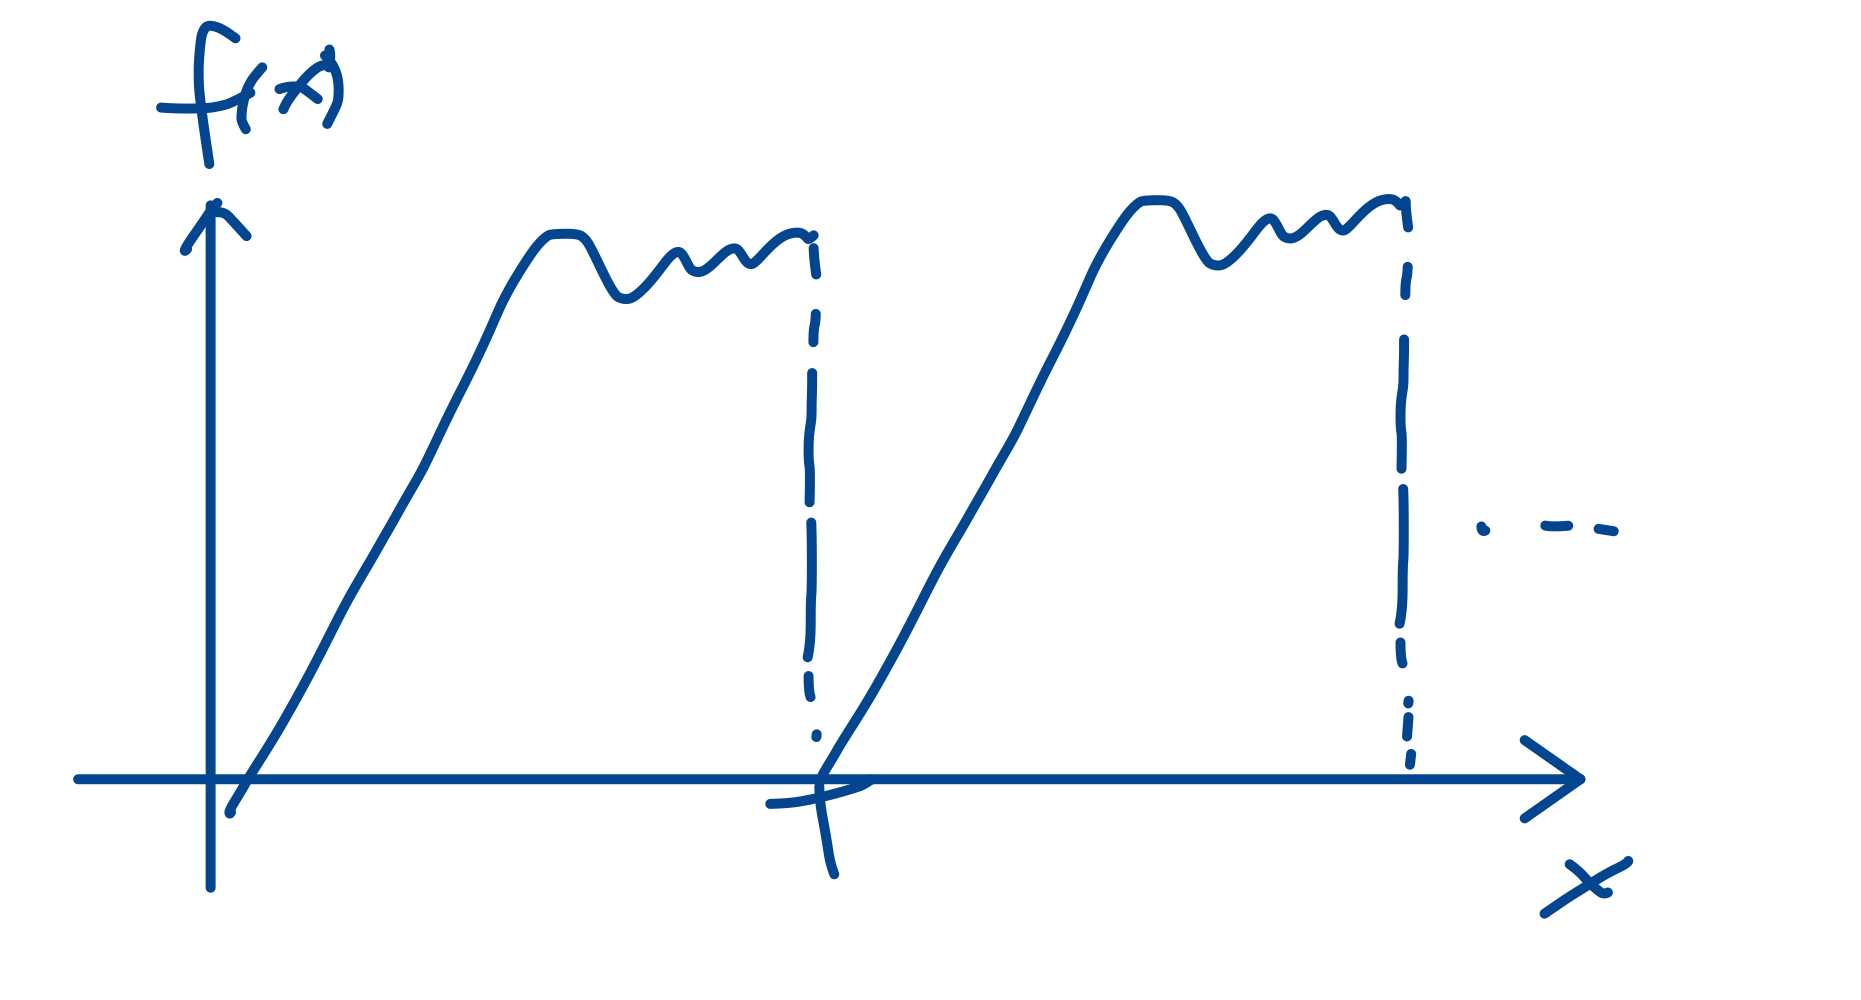
\includegraphics[scale=0.1]{methods1.jpeg}
\end{center}
Consider the set of functions 
\[
    g_n(x) = \cos \left( \frac{n\pi x}{L} \right),\quad h_n(x) = \sin \left( \frac{n\pi x}{L} \right).
\]
They are periodic on $ [0,2L] $ with period 2L.

Recall identities
\[
    \begin{aligned} \cos (A \pm B) &=\cos A \cos B \mp \sin A \sin B \\ \sin (A \pm B) &=\sin A \cos B \pm \cos A \sin B, \text { and so } \\ \cos A \cos B &=\frac{1}{2}[\cos (A-B)+\cos (A+B)] \\ \sin A \sin B &=\frac{1}{2}[\cos (A-B)-\cos (A+B)] \\ \sin A \cos B &=\frac{1}{2}[\sin (A+B)+\sin (A-B)] \end{aligned}
\]
Define an inner product of the set 
\[
    \langle f,g \rangle = \int_{0}^{2L} f(x)g(x)\,\mathrm{d}x.
\]
\begin{proposition}
    With this inner product, $g_n,h_n$ are mutually orthogonal on $ [0,2L) $.
\end{proposition}
\begin{proof}
    Claim that
    \begin{align}
        &\langle h_n,h_m \rangle = \begin{cases}
            L\delta_{nm} &\forall n,m\neq 0\\
            0 & m=0 \lor n=0\\
            \end{cases} \\
            &\langle g_n,g_m \rangle = \begin{cases}
            L \delta_{mn} &n,m\neq 0\\
            2L \delta_{0n} & m=0\\
            \end{cases} \\
            &\langle h_n,g_m \rangle =0
    \end{align}
    \textit{Proof of claim.} Note that for $n\neq m$,
    \begin{align*}
        \langle h_n,h_m \rangle &= \int_{0}^{2L} \sin \frac{n\pi x}{L} \sin \frac{m\pi x}{L} \,\mathrm{d}x\\ 
        &=\int_{0}^{2L} \frac{1}{2}\left( \cos \frac{(n-m)\pi x }{L}-\cos \frac{(n+m)\pi x}{L} \right) \,\mathrm{d}x\\ 
        &= \frac{1}{2} \left[ \frac{L}{(n-m)\pi}\sin \frac{(n-m)\pi x }{L}-\frac{L}{(n+m)\pi} \sin \frac{(n+m)\pi x }{L} \right]_0^{2L}\\ 
        &= \frac{1}{2}\left( \frac{L}{(n-m)\pi}\sin (2\pi(n-m))-\frac{L}{(n+m)\pi} \sin (2\pi(n+m)) \right)\\ 
        &=0.
    \end{align*}
    For $n=m$, 
    \begin{align*}
        \langle h_n,h_m \rangle &= \int_{0}^{2L} \sin^2 \frac{n\pi x}{L} \,\mathrm{d}x\\ 
        &= \int_{0}^{2L} \frac{1-\cos \frac{2n\pi x}{L}}{2} \,\mathrm{d}x\\ 
        &= L.
    \end{align*}
    This proves (1.1). The rest are similar.
\end{proof}
$g_n,h_n$ form a complete orthogonal set, i.e. they span the space of well-behaved periodic functions $ [0,2L) $ and they are linearly independent.

\subsection{Definition of Fourier series}
\ \vspace{-1.5em}
\begin{definition}
    We can express any well-behaved periodic function of period $2L$ as 
\begin{equation}\label{1.eq.4:FS}
    f(x) = \frac{1}{2}a_0 + \sum_{n=1}^{\infty} a_n \cos \left( \frac{n\pi x}{L} \right)+ \sum_{n=1}^{\infty} b_n \sin \left( \frac{n\pi x}{L} \right)
\end{equation}
where $a_n,b_n$ are constants such that RHS is convergent for all $x$ where $f$ is continuous. At a discontinuity $x$, the Fourier series approaches the midpoint of upper and lower limits at $x$, i.e. 
\[
    \frac{f(x_+)+f(x_-)}{2} = \frac{1}{2}a_0 + \sum_{n=1}^{\infty} a_n \cos \left( \frac{n\pi x}{L} \right)+ \sum_{n=1}^{\infty} b_n \sin \left( \frac{n\pi x}{L} \right).
\]
\end{definition}
Consider $ \langle h_n,f \rangle  $ and substitute in (1.4), we get 
\[
    \int_{0}^{2L} \sin \left( \frac{n \pi x}{L} \right) f(x) \,\mathrm{d}x = \sum_{m=1}^{\infty}Lb_m \delta_{nm} = Lb_n.
\]
Similar for $a_n$. We get
\begin{proposition}
    \begin{equation}
        \begin{aligned}
            &b_{n}=\frac{1}{L} \int_{0}^{2 L} f(x) \sin \left(\frac{n \pi x}{L}\right)\, \rmd x\\ &a_n = \frac{1}{L}\int_{0}^{2L} f(x) \cos \left( \frac{n \pi x}{L} \right) \,\mathrm{d}x
        \end{aligned}
    \end{equation}
\end{proposition}
\begin{note}
    \begin{enumerate}
        \item $a_n$ includes $n=0$ since $ \frac{1}{2}a_0 $ is the average of $f$, i.e.
        \[
            \langle f \rangle = \frac{1}{2L}\int_{0}^{2L} f(x) \,\mathrm{d}x.
        \]
        \item Range of integration can be changed as long as it has length $2L$. We usually consider $ \int_{-L}^{L} $.
        \item Can think of the Fourier series as the decomposition into harmonics. The simplest Fourier series are sines and cosines. e.g. $ \sin (3 \pi x/ L) $ has Fourier series $b_3=1$ and $ b_n=0,n\neq 3 ,a_n=0$.
    \end{enumerate}
\end{note}
\begin{example}[Sawtooth wave]
    Consider $f(x)=x,x\in [-L,L)$ and periodic elsewhere.
    \begin{center}
        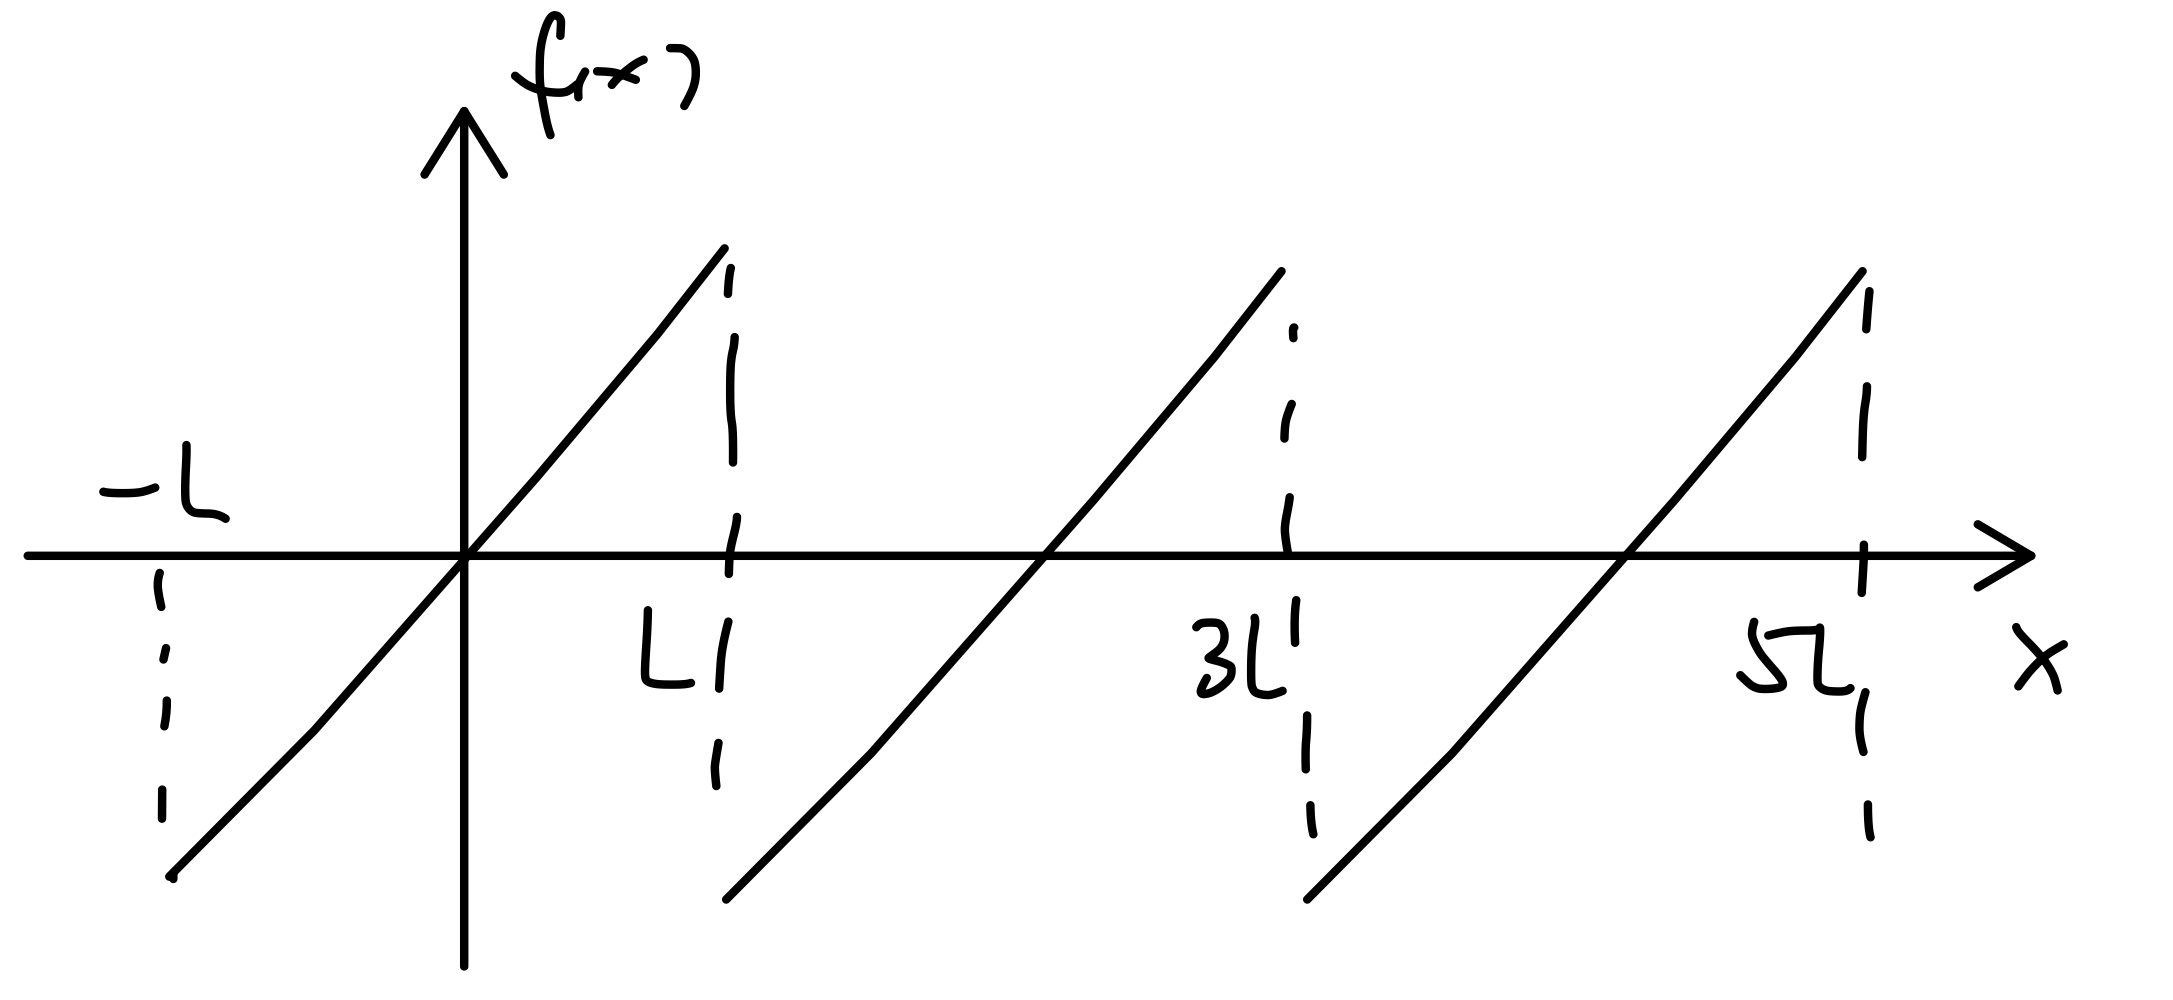
\includegraphics[scale=0.1]{methods2.jpeg}
    \end{center}
    We have 
    \begin{align*}
        a_n &= \frac{1}{L}\int_{-L}^{L} x\cdot \cos \left( \frac{n\pi x}{L} \right) \,\mathrm{d}x=0,\\ 
        b_n &= \frac{2}{L} \int_{0}^{L} x\cdot \sin \left( \frac{n\pi x}{L} \right) \,\mathrm{d}x = \frac{2L}{n\pi }(-1)^{n+1}.
    \end{align*}
    So the Fourier series is 
    \begin{equation}
        f(x) = \frac{2L}{\pi } \sum_{n=1}^{\infty}\frac{(-1)^{n+1}}{n}\sin \left( \frac{n\pi x}{L} \right).
    \end{equation}
\end{example}
\begin{note}
    As $n\to \infty$ in Fourier series,
    \begin{enumerate}
        \item The FS approximation improves (convergent where continuous).
        \item FS $ \to 0 $ at $x=L$, i.e. the midpoint of continuity.
        \item FS has a persistent \textit{overshoot} at $x=L$, which is approximately 9\% and is known as the \textit{Gibbs phenonenon}. See Example Sheet Q5.
    \end{enumerate}
\end{note}

\subsection{The Dirichlet Conditions and Fourier's Theorem}
A natural question is then which functions are allowed to have a proper Fourier series.
Surprisingly, a big, yet hard to precisely characterise, class of functions has a convergent Fourier series that has the desired properties.
This class even includes some classical counterexamples in analysis.
As an applied course, we will just look at some of the sufficient conditions.
\begin{theorem}[Fourier's Theorem]
    If $f$ is a bounded periodic function with period $2L$ with a finite number of minima, maxima, and discontinuities in $[0,2L)$, then its Fourier series converges to $f$ where it is continuous and converges to the average of the two side limits.
\end{theorem}
The conditions in this theorem is known as the Dirichlet conditions.
\begin{note}
    \begin{enumerate}
        \item These conditions are hella weak compared to our conditions for a function to have e.g. a Taylor series.
        However, pathological functions like $1/x,\sin(1/x),1_{\mathbb R\setminus\mathbb Q}(x)$ are excluded from these conditions.
        \item The converse is not true, as $\sin(1/x)$ has a Fourier series we desire.
    \end{enumerate}
\end{note}
\begin{proof}
    See Jeffery \& Jeffery book.
\end{proof}
Another subject of interest is the rate of convergence of a Fourier series.
Perhaps unsurprisingly, it depends on the smoothness of the function.
\begin{theorem}
    If $f(x)$ is $p^{th}$ differentiable but $f^{(p)}$ is not continuous, then its Fourier series converges as $O(n^{-(p+1)})$ as $n\to\infty$.
\end{theorem}
\begin{example}
    \begin{enumerate}
        \item  Consider the square wave
        $$f(x)=\begin{cases}
            1\text{, for $0\le x<1$}\\
            -1\text{, for $-1\le x<0$}
        \end{cases}$$
        That extends periodically with period $2$.
        Then it has a Fourier series
        \begin{equation}
            f(x)=4\sum_{m=1}^\infty\frac{\sin[(2m-1)\pi x]}{(2m-1)\pi}
        \end{equation}
        which, as one can see both from the preceding theorem (with $p=0$) and observation, converges slowly.
        \item Consider the general ``see-saw'' wave
        $$f(x)=\begin{cases}
            x(1-\xi)\text{, for $x\in[0,\xi)$}\\
            \xi(1-x)\text{, for $x\in[\xi,1)$}
        \end{cases}$$
        which extends as an odd periodic function with period $2$.
        This has Fourier series
        \begin{equation}
            f(x)=2\sum_{m=1}^\infty\frac{\sin (n\pi\xi)\sin (n\pi x)}{(n\pi)^2}
        \end{equation}
        which converges with $p=1$ in the preceding theorem.
        In particular, $\xi=1/2$ gives
        $$2\sum_{m=1}^\infty(-1)^{m+1}\frac{\sin[(2m-1)\pi x]}{[(2m-1)\pi]^2}$$
        which can be seen, immediately, that it converges faster than the series in the previous example.
        \item Take $f(x)=x(1-x)/2$ for $x\in[0,1)$ that extends as an odd periodic function with period $2$.
        Then its Fourier series is
        \begin{equation}
            f(x)=4\sum_{m=1}^\infty\frac{\sin[(2m-1)\pi x]}{[(2m-1)\pi]^3}
        \end{equation}
        which has $p=2$.
        \item Take $f(x)=(1-x^2)^2$, then $a_n=O(n^{-4})$.
    \end{enumerate}
\end{example}
Of course, we want to integrate and differentiate a Fourier series term-by-term.
Integration, as one expect, seldom yields problems as it imposed very few restrictions on the function.

And indeed, we are just going to assume we can integrate any Fourier series term-by-term and they guarantee to yield a smoother function, which satisfies the Dirichlet conditions if the original function does.

Differentiation is more problematic when doing it term-by-term.
\begin{example}
    Take the square wave again which is known to have Fourier series
    $$4\sum_{m=1}^\infty\frac{\sin[(2m-1)\pi x]}{(2m-1)\pi}$$
    which, after term-by-term differentiation, yields
    $$4\sum_{m=1}^\infty\cos[(2m-1)\pi x]$$
    which is clearly divergent.
    This is perhaps unsurprising as the original function is not even continuous.
\end{example}
\begin{theorem}
    If $f(x)$ is differentiable and both $f,f^\prime$ satisfy Dirichlet conditions, then we can differentiate the Fourier series of $f$ term-by-term to get the Fourier series of $f^\prime$.
\end{theorem}
\begin{example}
    If we differentiate the see-saw curve with $\xi=1/2$, then we will get an offset of the Fourier series of the square wave with $ \tilde{x}=x+1/2 $.
\end{example}
\subsection{Parseval's Theorem}
There is some interesting relation between the integral of the square of a function and the square of the Fourier coefficients of that function.
If the function is nice enough to have a nice enough Fourier series, then by orthogonality,
\begin{align*}
    \int_0^{2L}f(x)^2\,\mathrm dx&=\int_0^{2L}\left( \frac{a_0}{2}+\sum_{n\ge 1}a_n\cos\frac{n\pi x}{L}+\sum_{n\ge 1}b_n\sin\frac{n\pi x}{L} \right)^2\,\mathrm dx\\
    &=\int_0^{2L}\left( \frac{a_0^2}{4}+\sum_{n\ge 1}a_n^2\cos^2\frac{n\pi x}{L}+\sum_{n\ge 1}b_n^2\sin^2\frac{n\pi x}{L} \right)\,\mathrm dx\\
    &=L\left( \frac{a_0^2}{2}+\sum_{n\ge 1}(a_n^2+b_n^2) \right).
\end{align*}
This is also called the \textit{completeness relation} as the left hand side would be greater than or equal to the right hand side if any basis functions are missing from the series.
This is known as Parseval's Theorem.
\begin{theorem}[Parseval's Theorem]\label{parseval}
    For a nice enough function $f$ with Fourier coefficients $a_n,b_n$, we have
    \begin{equation}
        \int_0^{2L}f(x)^2\,\mathrm dx=L\left( \frac{a_0^2}{2}+\sum_{n\ge 1}(a_n^2+b_n^2) \right).
    \end{equation}
\end{theorem}
\begin{proof}
    Above.
\end{proof}
\begin{example}
    Consider the sawtooth curve with $f(x)=x,x\in[-L,L)$ with period $2L$.
    Then Parseval's Theorem reveals that
    $$\frac{2}{3}L^3=\int_{-L}^Lx^2\,\mathrm dx=L\sum_{n=1}^\infty\frac{4L^2}{n^2\pi^2}=\frac{4L^3}{\pi^2}\sum_{n=1}^\infty\frac{1}{n^2}\implies \sum_{n=1}^\infty\frac{1}{n^2}=\frac{\pi^2}{6}.$$
\end{example}
\begin{remark}
    If we think of the integral of the square as $ \langle f,f \rangle = \left\| f \right\| ^2  $, the $ L^2 $ norm, then Parseval's Theorem can be thought of an analog of Pythagoras' Theorem in this space of functions.
\end{remark}

\subsection{Alternative Fourier Series}
\paragraph{Fourier sines and cosines.}
Consider a function $f:[0,L)\to\mathbb R$.
We can extend $f$ to a periodic function of period $2L$ in two ways:
\begin{enumerate}
    \item We can require the function to be odd, then $a_n=0$ for all $n$ and
    \begin{equation}
        b_n=\frac{2}{L}\int_0^Lf(x)\sin\frac{n\pi x}{L}\,\mathrm dx
    \end{equation}
    and the Fourier series would be $\sum_{n\ge 1}b_n\sin(n\pi x/L)$, which is called a \textit{Fourier sine series}.
    The sawtooth function is an example of this.
    \item We can require the function to be even, then $b_n=0$ for all $n$ and
    \begin{equation}
        a_n=\frac{2}{L}\int_0^Lf(x)\cos\frac{n\pi x}{L}\,\mathrm dx
    \end{equation}
    So the Fourier series is $a_0/2+\sum_{n\ge 1}a_n\cos(n\pi x/L)$.
    This is called a \textit{Fourier cosine series}.
    $f(x)=(1-x^2)^2$ is an example (where $L=1$).
\end{enumerate}
\paragraph{Complex Fourier series.}
The actual thing we want is to represent the Fourier series more neatly in terms of exponentials.
We know that
$$\cos\frac{n\pi x}{L}=\frac{e^{in\pi x/L}+e^{-in\pi x/L}}{2},\sin\frac{n\pi x}{L}=\frac{e^{in\pi x/L}-e^{-in\pi x/L}}{2i}$$
So by writing $c_0=a_0/2$ and
$$c_m=\begin{cases}
    (a_m-ib_m)/2&\text{for $m>0$}\\
    (a_{-m}+ib_{-m})/2&\text{for $m<0$}
\end{cases}$$
we obtain
\begin{equation}
    f(x)=\frac{a_0}{2}+\sum_{n=1}^\infty a_n\cos\frac{n\pi x}{L}+\sum_{n=1}^\infty b_n\sin\frac{n\pi x}{L}=\sum_{m=-\infty}^\infty c_me^{im\pi x/L}
\end{equation}
Equivalently, if we extend our inner product to the complex functions
$$\langle f,g\rangle=\int_{-L}^Lf(x)\overline{g(x)}\,\mathrm dx$$
then we obtain
\begin{equation}
    c_m=\frac{1}{2L}\langle f(x),e^{im\pi x/L}\rangle=\frac{1}{2L}\int_{-L}^Lf(x)e^{-im\pi x/L}\,\mathrm dx
\end{equation}
because of orthogonality
\begin{equation}
    \langle e^{im\pi x/L},e^{in\pi x/L}\rangle= \int_{-L}^{L} e^{-im\pi x/L}e^{in\pi x/L} \,\mathrm{d}x=2L\delta_{mn}
\end{equation}
By thinking them as a set of basis of a space of nice-enough functions in the way we did for $\sin$ and $\cos$.
Parseval's Theorem can then be stated as
$$\int_{-L}^L|f(x)|^2\,\mathrm dx=2L\sum_{n=-\infty}^\infty|c_n|^2$$
\subsection{Some Motivations of Fourier Series}\ \vspace{-1.5em}
\begin{definition}
    The complex inner product $\langle\cdot\rangle:\mathbb C^N\times\mathbb C^N\to\mathbb C$ is defined by
    \begin{equation}
        \langle\mathbf{u},\mathbf{v}\rangle=\mathbf{u}^\dagger\mathbf{v}
    \end{equation}
\end{definition}
\begin{definition}
    An $N\times N$  matrix $A$ is \textit{self-adjoint} (or \textit{Hermitian}) if
    $$\forall\mathbf{u},\mathbf{v}\in\mathbb C^N,\langle A\mathbf{u},\mathbf{v}\rangle=\langle\mathbf{u},A\mathbf{v}\rangle.$$
\end{definition}
One can show that this is just saying $A^\dagger=A$.
It can be shown that
\begin{proposition}
    Let $A$ be a self-adjoint matrix. Then the eigenvalues $ \lambda_n $ and eigenvectors $ \bfv_n $ satisfy
    \begin{equation}
        A \bfv_n=\lambda_n\bfv_n
    \end{equation}
    and hence the followings hold:
    \begin{enumerate}[(i).]
        \item All eigenvalues are real for all $n$.
        \item Eigenvectors associated with different eigenvalues are orthogonal with respect to $\langle\cdot\rangle$.
        \item We can rescale to make an orthonormal basis of $\mathbb C^N$ of eigenvectors $\{\mathbf{v}_1,\ldots,\mathbf{v}_N\}$.
    \end{enumerate}
\end{proposition}
\paragraph{Recap of solving linear equations.}
Now, given any $\mathbf{b}$, if we want to solve for $\mathbf{x}$ in
\begin{equation}
    A\mathbf{x}=\mathbf{b}
\end{equation}
then a way to do it is to express $\mathbf{b}=\sum_nb_n\mathbf{v}_n$ and observe that if $\sum_nc_n\mathbf{v}_n$ is a solution then
$$\sum_nb_n\mathbf{v}_n=A\left(\sum_{n=1}^Nc_n\mathbf{v}_n\right)=\sum_{n=1}^Nc_n\lambda_n\mathbf{v}_n$$
where $\lambda_n$ is the eigenvalue associated with $\mathbf{v}_n$.
So if $A$ is nonsingular, then none of the $\lambda_n$ is zero and we can write $c_n=b_n/\lambda_n$ and get the solution
\begin{equation}
    \mathbf{x}=\sum_{n=1}^N\frac{b_n}{\lambda_n}\mathbf{v}_n
\end{equation}
This means we can solve an linear equation if there is a basis consisting of eigenvectors of the matrix.
\paragraph{Analogy to ODEs.}
Consider the differential operator
$$\mathcal Ly=-\frac{\mathrm d^2y}{\mathrm dx^2}$$
and suppose we want to solve
\begin{equation}
    \mathcal{L}y = f(x)\quad \text{subject to}\quad y(0)=y(L)=0.
\end{equation}
The related eigenvalue problem is then $\mathcal L y_n=\lambda_ny_n$ with $y_n(0)=y_n(L)=0$ which has solutions
\begin{equation}\label{1.eq.21}
    y_n(x)=\sin\frac{n\pi x}{L},\quad \lambda_n=\left( \frac{n\pi}{L} \right)^2.
\end{equation}
So we will want to write
\begin{align*}
    &y(x)=\sum_{n=1}^\infty c_n\sin\frac{n\pi x}{L},\\ 
    &f(x)=\sum_{n=1}^\infty b_n\sin\frac{n\pi x}{L},\\ 
    &b_n=\frac{2}{L}\int_0^Lf(x)\sin\frac{n\pi x}{L}\,\mathrm dx,
\end{align*}
assuming convergence.
Then this substitution yields
$$\sum_{n=1}^\infty b_n\sin\frac{n\pi x}{L}=\mathcal Ly=-\frac{\mathrm d^2y}{\mathrm dx^2}\left( \sum_{n=1}^\infty c_n\sin\frac{n\pi x}{L} \right)=\sum_{n=1}^\infty c_n\left( \frac{n\pi}{L} \right)^2\sin\frac{n\pi x}{L}$$
Hence, $c_n=b_n(L/(n\pi))^2$ by orthogonality, so we can get a particular solution of the problem in the form
\begin{equation}
    y(x)=\sum_{n=1}^\infty \frac{b_n}{\lambda_n}y_n = \sum_{n=1}^{\infty}b_n \left( \frac{L}{n\pi} \right)^2 \sin \frac{n\pi x}{L}.
\end{equation}
\begin{example}\label{odd_sq_fourier_ode}
    Consider the problem $ \mathcal{L}y=f(x) $ with $L=1$ and set $f$ to be the odd square wave with $f(x)=1$ for $x\in[0,1)$.
    This has Fourier series
    $$f(x)= 4\sum_{m=1}^\infty\frac{\sin[(2m-1)\pi x]}{(2m-1)\pi}.$$
    So the above discussion instantly yield a solution
    $$y(x)=\sum_{n=1}^\infty \frac{b_n}{\lambda_n}y_n=4\sum_{m=1}^\infty\frac{\sin[(2m-1)\pi x]}{[(2m-1)\pi]^3}$$
    which is the Fourier series of
    \begin{equation}
        y(x)=\frac{x(1-x)}{2}\quad \text{on}\quad[0,1)
    \end{equation}
    extending as an odd periodic function with period $2$.

    Indeed, as one can verifty, if we integrate $\mathcal L y=1$ directly with the appropriate boundary conditions, we can get basically the same solution.
\end{example}
\subsection{A Glimpse into Green's Functions}
In the problem $ \mathcal{L}y=f(x) $, fix $L=1$ and consider an odd function $f$.
We have
\begin{align}
    y(x)&=\sum_{n=1}^\infty\frac{b_n}{\lambda_n}\sin(\pi x)\nonumber\\
    &=\sum_{n=1}^\infty\frac{2}{(n\pi)^2}\left(\int_0^1f(\xi)\sin(n\pi\xi)\,\mathrm d\xi\right)\sin(n\pi x)\nonumber\\
    &=\int_0^12\sum_{n=1}^\infty\frac{\sin(n\pi x)\sin(n\pi\xi)}{(n\pi)^2}f(\xi)\,\mathrm d\xi\tag{Assume swapping limits}\\
    &=\int_0^1G(x,\xi)f(\xi)\,\mathrm d\xi
\end{align}
where
\begin{equation}
    G(x,\xi)=2\sum_{n=1}^\infty\frac{\sin(n\pi x)\sin(n\pi\xi)}{(n\pi)^2}.
\end{equation}
It is exactly the general see-saw wave
\begin{equation}
    G(x,\xi)=\begin{cases}
        x(1-\xi)\text{, for $x\in[0,\xi)$}\\
        \xi(1-x)\text{, for $x\in[\xi,1)$}
    \end{cases}
\end{equation}
This is the \textit{Green's function} for this ODE $-\rmd^2 y/\rmd x^2 =f(x)$.
One can actually solve this integral and get what we got in Example \ref{odd_sq_fourier_ode}.

\section{Sturm-Liouville Theory}
\subsection{Review of Second-Order Linear ODEs}
For a general inhomogeneous ODE $\mathcal Ly=f(x)$ where
\begin{equation}
    \mathcal Ly=\alpha(x)\frac{\mathrm d^2y}{\mathrm dx^2}+\beta(x)\frac{\mathrm dy}{\mathrm dx}+\gamma(x)y
\end{equation}
In general, the homogeneous equation
\begin{equation}
    \mathcal Ly=0
\end{equation}
has two linearly independent solutions $y_1,y_2$.
The complementary function
\begin{equation}
    y_c(x)=Ay_1+By_2
\end{equation}
for constants $A,B$ is then the general solution to $\mathcal Ly=0$ by linearity.

For the inhomogeneous problem 
\begin{equation}
    \mathcal Ly=f(x)
\end{equation}
If we can find a particular solution (aka particular integral) $y_p$ to $\mathcal Ly=f$, then
\begin{equation}
    y=y_p+y_c=y_p+Ay_1+By_2
\end{equation}
for $A,B$ constants is the general solution to $\mathcal Ly=f$ again by linearity.
Two pieces of boundary data is then needed to determine the constants $A,B$.

There are several types of boundary conditions.
\begin{itemize}
    \item The Dirichlet condition of specifying the function's value at the endpoints, \item The Neumann condition of specifying the derivative's values at the endpoints.
    \item Mixed conditions of above.
\end{itemize}

The sort of conditions we often consider are homogeneous conditions, i.e. the function vanishes at the endpoints.
The reason of it is that it allows the \textit{superposition} of solutions in a linear DE.
What if we come across a inhomogeneous condition?
We can use the complementary solution to cancel stuff out.

Sometimes, we specify initial data of the function and its derivative as boundary conditions.

Another matter of interest is the general eigenvalue problem.
To solve $\mathcal Ly=f$ using eigenvalue decompositions like we did previously, we must first solve (subject to boundary conditions) the related eigenvalue problem
\begin{equation}
    \mathcal Ly=\alpha(x)\frac{\mathrm d^2y}{\mathrm dx^2}+\beta(x)\frac{\mathrm dy}{\mathrm dx}+\gamma(x)y=-\lambda\rho(x)y
\end{equation}
where $\rho$ is nonegative.
This form often occurs after seperation of variables in a PDE.
\subsection{Self-Adjoint Operators}\ \vspace{-1.5em}
\begin{definition}
    For two functions $f,g:[a,b]\to\mathbb C$ we define their inner product to be
    $$\langle f,g\rangle=\int_a^bf^*(x)g(x)\,\mathrm dx$$
\end{definition}

\begin{definition}[Sturm-Liouville form]
    An ODE $ \mathcal{L}y=f(x) $ can be written as the \textit{Sturm-Liouville form} if $ \mathcal{L} $ can be written as
    \[
        \mathcal{L}y=-(py')'+qy,
    \]
    where $ p,q$ are functions, and the ODE $ \mathcal{L}y=f(x) $ can be written as 
    \begin{equation}
        \mathcal{L}y=-(py')'+qy=\lambda w y,
    \end{equation}
    where $w$ is a nonnegative weight function.
\end{definition}

We can guarantee to rewrite the original eigenvalue problem into the Sturm-Liouville form.

\paragraph{Integrating factor} How to convert a second order linear ODE to this form?
Simply multiply the diffential equation by an integrating factor $F$ that will be specified later and we can write
\begin{align*}
    &F \alpha y''+F \beta y'+ F \gamma y = -\lambda F \rho y\\ 
    \implies&\frac{\mathrm d}{\mathrm dx}(F\alpha y^\prime)-F^\prime\alpha y^\prime-F\alpha^\prime y^\prime+F\beta y^\prime+F\gamma y=-\lambda F\rho y.
\end{align*}
So to eliminate the $y^\prime$ terms, we set
\begin{equation}
    F^\prime\alpha y^\prime+F\alpha^\prime y^\prime-F\beta y^\prime=0 \Longrightarrow  F(x)=\exp\left(\int\frac{\beta-\alpha^\prime}{\alpha}\,\mathrm dx\right)
\end{equation}
which reduced the equation to
$$(F\alpha y^\prime)^\prime+F\gamma y=-\lambda F\rho y \Longleftrightarrow -(py')'+qy=\lambda w y,$$
setting $p=F\alpha,q=-F\gamma$ and $w=F\rho\ge 0$.
\begin{example}
    Consider the Hermite equation that appears in quantum mechanics
    $$y^{\prime\prime}-2xy^\prime+2ny=0$$
    Then $\alpha=1,\beta=-2x,\gamma=0,\lambda\rho=2n$, so the above procedure translates this to the Sturm-Liouville form
    \begin{equation}\label{2.eq.9}
        \mathcal Ly=(-e^{-x^2}y^\prime)^\prime=2ne^{-x^2}y
    \end{equation}
\end{example}
\subsubsection*{Boundary conditions}

\begin{definition}[Self-adjoint operators]
    Let $\mathcal L:C\to C$ be an operator, where $C$ on a class of functions $[a,b]\to\mathbb C$ equipped with the inner product above.
    $\mathcal L$ is \textit{self-adjoint} if $\langle y_1,\mathcal Ly_2\rangle=\langle\mathcal Ly_1,y_2\rangle$ for any $y_1,y_2\in C$. Equivalently,
    \begin{equation}
        \int_{a}^{b} y_1^*(x)\mathcal{L}y_2(x) \,\mathrm{d}x = \int_{a}^{b} (\mathcal{L}y_1(x))^* y_2(x) \,\mathrm{d}x
    \end{equation}
\end{definition}

If we let $\mathcal L$ be the operator in the Strum-Liouville form, then
\begin{align}
    \langle y_1,\mathcal Ly_2\rangle-\langle\mathcal Ly_1,y_2\rangle&=\int_a^b[-y_1(py_2^\prime)^\prime+y_1qy_2+y_2(py_1^\prime)^\prime-y_2qy_1]\,\mathrm dx\nonumber\\
    &=\int_a^b[-y_1(py_2^\prime)^\prime+y_2(py_1^\prime)^\prime]\,\mathrm dx\nonumber\\
    &=\int_a^b[-(y_1(py_2^\prime)^\prime+y_1^\prime py_2^\prime)+(y_2(py_1^\prime)^\prime+y_2^\prime py_1^\prime)]\,\mathrm dx\nonumber\\
    &=\int_a^b[-(py_1y_2^\prime)^\prime+(py_1^\prime y_2)^\prime]\,\mathrm dx\nonumber\\
    \implies \langle y_1,\mathcal Ly_2\rangle-\langle\mathcal Ly_1,y_2\rangle&=[-py_1y_2^\prime+py_1^\prime y_2]_a^b
\end{align}
So for this operator to be self-adjoint, we need some good enough boundary conditions so that enough stuff vanishes.
This includes homogeneous boundary condition $y(a)=y(b)=0$ or $y^\prime(a)=y^\prime(b)=0$ or mixed $y+ky^\prime=0$ etc.

We say a Sturm-Liouville problem is \textit{regular} if the boundary conditions are homogeneous.
Periodic boundary conditions also work, where we can take $y(a)=y(b)$ and the derivatives are specified (or periodic) at the boundary.
There can also be singular points of this ODE, where $p(a)=p(b)=0$.
We can have combinations of above too.

\subsection{Properties of Self-Adjoint Operators}
Analogous to the finite dimensional case, we have
\begin{theorem}\label{self-adjoint}
    For a sufficiently nice self-adjoint operator $\mathcal L$ on a sufficiently nice space of functions:
    \begin{enumerate}[(a)]
        \item Eigenvalues of $\mathcal L$ are real.
        \item Eigenfunctions of it with different eigenvalues are orthogonal with respect to the weight $w$.
        \item We can take the eigenfunctions as a set of basis for the function space, just like Fourier series.
    \end{enumerate}
\end{theorem}
\begin{proof}[Proof of (a)]
    Given
    \begin{equation}\label{2.eigenproblem}
        \mathcal Ly=\lambda wy
    \end{equation}
    taking complex conjugate gives $\mathcal Ly^*=\lambda^*wy^*$.
    Hence as $\mathcal L$ is self-adjoint,
    $$0=\int_a^b(y^*\mathcal Ly-y\mathcal Ly^*)\,\mathrm dx=(\lambda-\lambda^*)\int_a^bw|y|^2\,\mathrm dx$$
    which means $\lambda=\lambda^*$, so $\lambda$ is real.
\end{proof}
If $\lambda$ is non-degenerate (simple), i.e. it has a one-dimensional eigenspace, then $y$ is guaranteed to be real.
Even if it has dimension $2$ (not more because the ODE is second order), we can still find two real functions as basis of the eigenspace. Hence from now on, we assume the eigenfunctions to be real.

Also, by considering $u\mathcal Lv-v\mathcal Lu=(-p(uv^\prime-u^\prime v))^\prime$, one can show that a regular Sturm-Liouville problem always has all eigenvalues simple.

\begin{proof}[Proof of (b)]
    Suppose $\mathcal Ly_m=\lambda_mwy_m$ and $\mathcal Ly_n=\lambda_nwy_n$, then
    \begin{equation}\label{2.eq.13}
        0=\int_a^by_n\mathcal Ly_m-y_m\mathcal Ly_n\,\mathrm dx=(\lambda_m-\lambda_n)\int_a^bwy_ny_m\,\mathrm dx
    \end{equation}
    But $\lambda_m$ and $\lambda_n$ are distinct.
    The claim follows.
\end{proof}

\begin{definition}
    The inner product of $y_1,y_2:[a,b]\to\mathbb C$ with respect to weight $w:[a,b]\to\mathbb R_{\ge 0}$ is
    \begin{equation}
        \langle f,g\rangle_w=\int_a^bwf^*g\,\mathrm dx=\langle wf,g\rangle=\langle f,wg\rangle
    \end{equation}
\end{definition}

So the orthogonality in (\ref{2.eq.13}) becomes 
\begin{equation}
    \langle y_n,y_m \rangle _w = 0,\quad \forall n\neq m.
\end{equation}

\begin{remark}
    Watch the weight!
\end{remark}

As an aside, we do not really need the weight function in order to formulate Sturm-Liouville theory, since we can do the transformation $\tilde{y}=\sqrt{w}y$ and replace $\mathcal Ly$ by $(1/\sqrt{w})\mathcal L(\tilde{y}/\sqrt{w})$.
Yet the analytic property is generally simpler if we keep $w$.
\begin{example}
    For the Hermite equation \ref{2.eq.9}, we can eliminate $ w $ with $ \tilde{y}=e^{-x^2/2}y $ to find 
    \[
        \tilde{\mcL} = -\tilde{y}''+(x^2-1)\tilde{y}=2n \tilde{y}.
    \]
\end{example}
\subsection{Eigenfunction expansion}
Completeness ((c) in theorem \ref{self-adjoint}) implies we can approximate any well-behaved $f(x)$ on $ [a,b] $ by the series 
\begin{equation}
    f(x)=\sum_{n=1}^\infty a_ny_n(x)
\end{equation}
where $y_n$ is a set of eigenfunctions of some self-adjoint operator.
To find the coefficients $a_n$, we can use the orthogonality (\ref{2.eq.13}) to get
\[
    \int_{a}^{b} w(x)y_m(x)\cdot f(x) \,\mathrm{d}x = \sum_{n=1}^{\infty}a_n \int_{a}^{b} wy_ny_m \,\mathrm{d}x = a_m\int_a^bwy_m^2\,\mathrm dx
\]
Hence 
\begin{equation}\label{2.eq.17}
    a_n=\left(\int_a^bwy_nf\,\mathrm dx\middle)\right/\left(\int_a^bwy_n^2\,\mathrm dx\right)
\end{equation}
It's a common practice not to normalise the eigenfunctions as it is not really always clean.
Of course, if we want, we can always write down
\[
    Y_n=y_n\left/\sqrt{\int_a^bwy_n^2\,\mathrm dx}\right.
\]
So that 
\begin{equation}
    \langle Y_n,Y_m \rangle =\delta_{nm}
\end{equation}
are orthonormal with 
\[
    f(x) = \sum_{n=1}^{\infty}A_nY_n(x)\quad \text{and}\quad A_n = \int_{a}^{b} w(x)Y_n(x)f(x) \,\mathrm{d}x
\]
\begin{example}
    Recall the particular operator already in Sturm-Liouville form $\mathcal Ly=-y^{\prime\prime}$, then (with appropriate boundary conditions) we can easily get the eigenvalues $\lambda_n=(n\pi/L)^2$ and eigenfunctions being the trigonometrics.
    This just reproduces the Fourier series.
\end{example}
\subsection{Completeness and Parseval's Identity}
We expand
\begin{align*}
    &\int_a^bw\left( f(x)-\sum_{n=1}^\infty a_ny_n \right)^2\,\mathrm dx\\
    =&\int_a^bw\left( f^2-2f\sum_{n=1}^\infty a_ny_n+\sum_{n=1}^\infty a_n^2y_n^2 \right)\,\mathrm dx\tag{Last term by orthogonality} \\    
    =&\int_a^bwf^2\,\mathrm dx-\sum_{n=1}^\infty a_n^2\int_a^bwy_n^2\,\mathrm dx\tag{By \ref{2.eq.17}}
\end{align*}
If the eigenfunctions are complete, then the series expansion converges, and thus the above expansion is 0 and 

\begin{align}\label{2.eq.19}
    \int_a^bwf^2\,\mathrm dx&=\sum_{n=1}^\infty a_n^2\int_a^bwy_n^2\,\mathrm dx\\ 
    &=\sum_{n=1}^\infty A_n^2\text{ for unit normal $Y_n$}\nonumber
\end{align}
Note that $\int_a^bwy_n^2\,\mathrm dx$ becomes $L$ for Fourier series.

If some of the eigenfunctions are missing from the series, then this gives
$$\int_a^bwf^2\,\mathrm dx\ge\sum_{n=1}^\infty A_n^2$$
This is known as Bessel's Inequality.
\paragraph{Calculating the error}
Consider the partial sums $\sum_{n\le N}a_ny_n$, then we shall have
\begin{equation}\label{2.eq.20}
    f(x) = \lim_{N \to \infty} S_N(x)
\end{equation}
Convergence is defined in terms of the \textit{mean square error}
\[
    \epsilon_N=\int_a^bw[f(x)-S_N(x)]^2\,\mathrm dx\to 0,N\to\infty
\]
This global definition of convergence in mean is not the pointwise convergence of Fourier series, which converges to all the continuous points of $f$.

An interesting question is that, while we know (maybe) the series converges as we want, if we truncate the sequence in some $N$, would the coefficients $\{a_n\}_{n\le N}$ provide the best approxmation (with respect to the error defined in this way) of that particular partial sum, or a different set of partial coefficient will yield a better result?
The answer is yes. 
\begin{claim}
    The error in partial sums (\ref{2.eq.20}) is minimised by $a_n$ in (\ref{2.eq.19}) for $ N= \infty  $ expansion.
\end{claim}
\begin{proof}
    Differentiate wrt $a_n$ gives
    $$\frac{\partial\epsilon_N}{\partial a_n}=-2\int_a^bwy_n\left( f-\sum_{k=1}^Na_ky_k \right)\,\mathrm dx=-2\int_a^bwfy_n-a_nwy_n^2\,\mathrm dx$$
    which is zero when $a_n$ is of the expression in (\ref{2.eq.17}).
    We can see it is indeed a minimum by observing that
    $$\frac{\partial^2\epsilon_N}{\partial a_n^2}=2\int_a^bwy_n^2\,\mathrm dx\ge 0$$
    This answers our question.
\end{proof}
\subsection{Legendre's Equation}
Take the usual spherical polar coordinate
$$\begin{cases}
    x=r\sin\theta\cos\phi\\
    y=r\sin\theta\sin\phi\\
    z=r\cos\theta
\end{cases}$$
where Laplace's equation $\laplacian u=0$ translates to
$$\frac{1}{r^2}\frac{\partial}{\partial r}\left( r^2\frac{\partial u}{\partial r} \right)+\frac{1}{r^2\sin\theta}\frac{\partial}{\partial\theta}\left( \sin\theta\frac{\partial u}{\partial\theta} \right)+\frac{1}{r^2\sin^2\theta}\frac{\partial^2u}{\partial\phi^2}=0$$
Seperation of variables $u=R(r)\Theta(\theta)\Phi(\phi)$ then gives
$$\frac{1}{\sin\theta}(\Theta^\prime\sin\theta)^\prime+\left( K-\frac{m^2}{\sin^2\theta} \right)\Theta=0$$
where $K,m$ are constants which essentially makes it an eigenvalue problem.

Now the transformation $x=\cos\theta\in[-1,1]$ and renaming $\Theta$ as $y$ then gives Legendre's Equation
\begin{equation}\label{2.eq.21:legendre}
    (1-x^2)y^{\prime\prime}-2xy^\prime+\lambda y=0
\end{equation}
where $\lambda$ is a constant which is again intepreted as an eigenvalue.
This is already in Strum-Liouville form by taking $p=1-x^2,q=0,w=1$.
Now $p=1-x^2$ vanishes at the boundary $\pm 1$, so this equation has to be self-adjoint.
We assume that $y$ is bounded near the boundary. (Regular singular point)

We now seek a power series solution to the problem.
If we set
$$y=\sum_{n=0}^\infty c_nx^n$$
Then substitution gives 
\begin{align}\label{2.eq.22}
    &(1-x^2)\sum_n n(n-1)c_nx^{n-2}-2x \sum_n c_n x^{n-1} + \lambda \sum_n c_n x^n=0\nonumber\\
    \Longrightarrow & (n+2)(n+1)c_{n+2}-n(n-1)c_n-2nc_n+\lambda c_n=0\nonumber\\ 
    \implies &c_{n+2}=\frac{n(n+1)-\lambda}{(n+1)(n+2)}c_n
\end{align}
Specifying $c_0,c_1$ gives 2 independent solution near $ x=0 $:
\begin{align*}
    y_{\text{even}}&=c_0\left( 1+\frac{(-\lambda)}{2!}x^2+\frac{(6-\lambda)(-\lambda)}{4!}x^4+\cdots \right)\\
    y_{\text{odd}}&=c_1\left( x+\frac{2-\lambda}{3!}x^3+\cdots \right)
\end{align*}
Note that $c_{n+2}/c_n\to 1$, so the both series has radius of convergence $1$ but they diverges at $x=\pm 1$.

These series may not be infinite.
If $\lambda=l(l+1)$ for some $l\in\mathbb N$, then one of these two series will terminate and give a polynomial solution.
These polynomials are called \textit{Legendre polynomials} $P_l(x)$ which are eigenfunctions of the Legendre equation (\ref{2.eq.21:legendre}).

Conventionally we normalise $P_l$ by requiring $P_l(1)=1$.
One can check that this restricts $P_l([-1,1])\subset [-1,1]$ and $|P_l(-1)|=1$.
By calculation we have
\begin{align*}
    P_{0}(x)&=1\\ 
    P_{1}(x)&=x\\ 
    P_{2}(x)&=\frac{1}{2}\left(3 x^{2}-1\right)\\ 
    P_{3}(x)&=\frac{1}{2}\left(5 x^{3}-3 x\right)
\end{align*}
Note that 
\begin{enumerate}
    \item $P_l$ has $l$ roots in $[-1,1]$.
    \item $P_l$ is odd if $l$ is odd, and even when $l$ is even.
\end{enumerate}

\subsection{Properties of Legendre polynomials}
Since Legendre polynomials come from a self-adjoint operator, they must have certain conditions, such as orthogonality.
\begin{proposition}
    For \( n \neq m \), $\displaystyle \int_{-1}^1 P_n P_m \dd{x} = 0$. 
\end{proposition}
They are also normalisable,
\begin{proposition}
    $\displaystyle 
	\int_{-1}^1 P_n^2 \dd{x} = \frac{2}{2n+1}$
\end{proposition}
We can prove this with Rodrigues' formula:
\begin{proposition}
    $\displaystyle P_n(x) = \frac{1}{2^n n!} \qty( \dv{x} )^n (x^2 - 1)^n$ 
\end{proposition}
Alternatively we could use a generating function:
\begin{proposition}
    \begin{align*}
        \sum_{n=0}^\infty P_n(x) t^n = \frac{1}{\sqrt{1 - 2xt + t^2}} & = 1 + \frac{1}{2}\qty(2xt - t^2) + \frac{3}{8}\qty(2xt - t^2)^2 + \dots \\
                                                                      & = 1 + xt + \frac{1}{2}\qty(3x^2 - 1)t^2 + \dots
    \end{align*}
\end{proposition}
There are some useful recursion relations.
\begin{proposition}\
    \begin{enumerate}[(i)]
        \item $ \ell(\ell + 1) P_{\ell + 1} = (2 \ell + 1) x P_\ell(x) - \ell P_{\ell - 1}(x) $
        \item $\displaystyle (2\ell + 1)P_\ell(x) = \dv{x} \qty[ P_{\ell + 1}(x) - P_{\ell - 1}(x) ]$.
    \end{enumerate}
\end{proposition}

\subsection{Eigenfunction expansion}
Any (well-behaved) function on \( [-1,1] \) can be expressed as
\[
	f(x) = \sum_{\ell = 0}^\infty a_\ell P_\ell(x)
\]
where
\[
	a_\ell = \frac{2\ell + 1}{2} \int_{-1}^1 f(x) P_\ell(x) \dd{x}
\]
with no boundary conditions (e.g.\ periodicity conditions) on \( f \).

\subsection{S-L Theory on inhomogeneous ODEs}

\paragraph{Solve ODEs using SL theory} Consider the problem
\[
	\mathcal L y = f(x) \equiv w(x) F(x)
\]
on \( x \in [a,b] \) assuming homogeneous boundary conditions.
Given eigenfunctions \( y_n(x) \) satisfying \( \mathcal L y_n = \lambda_n w y_n \), we wish to expand this solution as
\[
	y(x) = \sum_n c_n y_n(x)
\]
and
\[
	F(x) = \sum_n a_n y_n(x)
\]
where \( a_n \) are known and \( c_n \) are unknown:
\[
	a_n = \frac{\int_a^b w F y_n \dd{x}}{\int_a^b w y_n^2 \dd{x}}
\]
Substituting,
\[
	\mathcal L y = \mathcal L \sum_n c_n y_n = w \sum_n c_n \lambda_n y_n = w \sum_n a_n y_n
\]
By orthogonality,
\[
	c_n \lambda_n = a_n \implies c_n = \frac{a_n}{\lambda_n}
\]
In particular,
\[
	y(x) = \sum_{n=1}^\infty \frac{a_n}{\lambda_n}y_n(x)
\]
\paragraph{Generalisation} Driving force often induces a linear response term \( \widetilde\lambda w y \).
\[
	\mathcal L y - \widetilde \lambda w y = f(x)
\]
where \( \widetilde \lambda \neq \lambda \). 
The solution becomes
\[
	y(x) = \sum_{n=1}^\infty \frac{a_n}{\lambda_n - \widetilde \lambda} y_n(x)
\]

\subsection{Integral solutions and Green's function}
Recall that
\[
	y(x) = \sum_{n=1}^\infty \frac{a_n}{\lambda_n} y_n(x) = \sum_n \frac{y_n(x)}{\lambda_n  N_n} \int_a^b w(\xi) F(\xi) y_n(\xi) \dd{\xi}
\]
where
\[
	N_n = \int w y_n^2 \dd{x}
\]
This then gives
\[
	y(x) = \int_a^b \underbrace{\sum_{n=1}^\infty \frac{y_n(x) y_n(\xi)}{\lambda_n N_n}}_{G(x,\xi)} \underbrace{w(\xi) F(\xi)}_{f(\xi)} \dd{\xi} = \int_a^b G(x;\xi) f(\xi) \dd{\xi}
\]
where
\[
	G(x,\xi) = \sum_{n=1}^\infty \frac{y_n(x) y_n(\xi)}{\lambda_n N_n}
\]
is the eigenfunction expansion of the \textbf{Green's function}.
Note that the Green's function does not depend on \( f \), but only on \( \mathcal L \) and the boundary conditions.
In this sense, it acts like an inverse operator
\[
	\mathcal L^- \equiv \int \dd{\xi} G(x,\xi)
\]
analogously to how \( Ax = b \implies x = A^{-1} b \) for matrix equations.

\clearpage

\part{PDEs on bounded domains}
\section{The Wave Equation}
\subsection{Waves on an elastic string: physical derivation}
Consider a small displacement \( y(x,t) \) on a stretched string with fixed ends at \( x = 0 \) and \( x = L \), that is, with boundary conditions \( y(0,t) = y(L,t) = 0 \).
We can determine the string's motion for specified initial conditions \( y(x,0) = p(x) \) and \( \pdv{y}{t}(x,0) = q(x) \).

We derive the equation of motion governing the motion of the string by balancing forces on a string segment \( (x,x+\delta x) \) and take the limit as \( \delta x \to 0 \).
Let \( T_1 \) be the tension force acting to the left at angle \( \theta_1 \) from the horizontal.
Analogously, let \( T_2 \) be the rightwards tension force at angle \( \theta_2 \).
We assume at any point on the string that \( \abs{\pdv{y}{x}} \ll 1 \), so the angles of the forces are small.
In the \( x \) dimension,
\[
	T_1 \cos \theta_1 = T_2 \cos \theta_2 \implies T_1 \approx T_2 = T
\]
So the tension \( T \) is constant up to an error of order \( O\qty(\abs{\pdv{y}{x}
}^2) \).
In the \( y \) dimension, since \( \theta \) are small,
\[
	F_T = T_2 \sin \theta_2 - T_1 \sin \theta_1 \approx T \qty(\eval{\pdv{y}{x}}_{x + \delta x} - \eval{\pdv{y}{x}}_x) \approx T \pdv[2]{y}{x} \delta x
\]
By \( F = ma \),
\[
	F_T + F_g = (\mu \delta x) \pdv[2]{y}{t} = T \pdv[2]{y}{x} \delta x - g \mu \delta x
\]
where \( F_g \) is the gravitational force and \( \mu \) is the linear mass density.
We define the wave speed as
$ c = \sqrt{T/\mu} $
and find
\[
	\pdv[2]{y}{t} = \frac{T}{\mu} \pdv[2]{y}{x} - g = c^2 \pdv[2]{y}{x}-g
\]
We often assume gravity is negligible to produce the pure wave equation
\[
	\frac{1}{c^2} \pdv[2]{y}{t} = \pdv[2]{y}{x} 
\]

\subsection{Separation of variables}

Consider a separable form:
\[
	y(x,t) = X(x) T(t)
\]
Substituting into the wave equation,
\[
	\frac{1}{c^2} \ddot y = y'' \implies \frac{1}{c^2} X \ddot T = X'' T
\]
Then
\[
	\frac{1}{c^2}\frac{\ddot T}{T} = \frac{X''}{X}
\]
However, \( \frac{\ddot T}{T} \) depends only on \( t \) and \( \frac{X''}{X} \) depends only on \( x \).
Thus, both sides must be equal to some \textbf{separation constant} \( -\lambda \).
\[
	\frac{1}{c^2}\frac{\ddot T}{T} = \frac{X''}{X} = -\lambda \implies X'' + \lambda X = 0;\quad \ddot T + \lambda c^2 T = 0
\]

\subsection{Boundary conditions and normal modes}

First look at the spatial part of the solution.

One of \( \lambda > 0, \lambda < 0, \lambda = 0 \) must be true.
The boundary conditions restrict the possible \( \lambda \).
\begin{enumerate}[align=left]
	\item[(1) \( \lambda < 0 \)] Take \( \chi^2 = -\lambda \).
	      Then,
	      \[
		      X(x) = Ae^{\chi x} + Be^{-\chi x} = \tilde{A} \cosh (\chi x) + \tilde{B} \sinh (\chi x)
	      \]
	      The boundary conditions are \( x(0) = x(L) = 0 \), so only the trivial solution is possible: \( \tilde{A} = \tilde{B} = 0 \).
	\item[(2) \( \lambda = 0 \)] Then
	      \[
		      X(x) = Ax + B
	      \]
	      Again, the boundary conditions impose \( A = B = 0 \) giving only the trivial solution.
	\item[(3) \( \lambda > 0 \)]
	      \[
		      X(x) = A \cos \qty(\sqrt{\lambda} x) + B \sin \qty(\sqrt{\lambda} x)
	      \]
	      The boundary conditions give
	      \[
		      A = 0,\quad B \sin \qty(\sqrt{\lambda} L) = 0 \implies \sqrt{\lambda} L = n \pi
	      \]
\end{enumerate}
The following are the eigenfunctions and eigenvalues.
\[
	X_n(x) = B_n \sin \frac{n \pi x}{L};\quad \lambda_n = \qty(\frac{n \pi}{L})^2
\]
These are also called the \textbf{normal modes} of the system.
The spatial shape in \( x \) does not change in time, but the amplitude may vary.
The \textbf{fundamental mode}, or \textbf{first harmonic}, is the lowest frequency of vibration, given by
\[
	n = 1 \implies \lambda_1 = \frac{\pi^2}{L^2}
\]
The \textbf{second mode}, or \textbf{overtone}, is the first overtone, and is given by
\[
	n = 2 \implies \lambda_2 = \frac{4\pi^2}{L^2}
\]
and so on. 

\subsection{Initial conditions and temporal solutions}
Substituting \( \lambda_n \) into the time ODE,
\[
	\ddot T + \frac{n^2 \pi^2 c^2}{L^2}T = 0
\]
Hence,
\[
	T_n(t) = C_n \cos \left(\frac{n \pi c t}{L}\right) + D_n \sin \left(\frac{n \pi c t}{L}\right)
\]
Therefore, a specific solution of the wave equation satisfying the boundary conditions is (absorbing the \( B_n \) into the \( C_n, D_n \)):
\[
	y_n(x,t) = T_n(t) X_n(x) = \qty(C_n \cos \left(\frac{n \pi c t}{L}\right) + D_n \sin \left(\frac{n \pi c t}{L}\right)) \sin \left(\frac{n \pi x}{L}\right)
\]
To find a particular solution for a given set of initial conditions, we must consider a linear superposition of all possible \( y_n \).
\[
	y(x,t) = \sum_{n=1}^\infty \qty(C_n \cos \left(\frac{n \pi c t}{L}\right) + D_n \sin \left(\frac{n \pi c t}{L}\right)) \sin \left(\frac{n \pi x}{L}\right)
\]
By construction, this \( y(x,t) \) satisfies the boundary conditions, so now we can impose the initial conditions.
\[
	y(x,0) = p(x) = \sum_{n=1}^\infty C_n \sin \left(\frac{n \pi x}{L}\right)
\]
We can find the \( C_n \) using standard Fourier series techniques, since this is exactly a half-range sine series.
Further,
\[
	\pdv{y(x,0)}{t} = q(x) = \sum_{n=1}^\infty \frac{n \pi c}{L} D_n \sin \left(\frac{n \pi x}{L}\right)
\]
Again we can solve for the \( D_n \) in a similar way.
In particular,
\[
	C_n = \frac{2}{L} \int_0^L p(x) \sin \left(\frac{n \pi x}{L}\right) \dd{x}
\]
\[
	D_n = \frac{2}{n \pi c} \int_0^L q(x) \sin \left(\frac{n \pi x}{L}\right) \dd{x}
\]
\begin{example}
	Consider the initial condition of a see-saw wave parametrised by \( \xi \), and let \( L = 1 \).
	This can be visualised as plucking the string at position \( \xi \).
	\[
		y(x,0) = p(x) = \begin{cases}
			x(1-\xi) & 0 \leq x < \xi \\
			\xi(1-x) & \xi \leq x < 1
		\end{cases}
	\]
	We also define
	\[
		\pdv{y(x,0)}{t} = q(x) = 0
	\]
	The Fourier series for \( p \) is given by
	\[
		C_n = \frac{2 \sin (n \pi \xi)}{(n \pi)^2};\quad D_n = 0
	\]
	Hence the solution to the wave equation is
	\[
		y(x,t) = \sum_{n=1}^\infty \frac{2}{(n \pi)^2} \sin (n \pi \xi) \sin (n \pi x) \cos (n \pi c t)
	\]
\end{example}

\subsection{Separation of variables: algorithm}
A general strategy for solving higher-dimensional partial differential equations is as follows.
\begin{enumerate}
	\item Obtain a linear PDE system, using boundary and initial conditions.
	\item Separate variables to yield decoupled ODEs.
	\item Impose homogeneous boundary conditions to find eigenvalues and eigenfunctions.
	\item Use these eigenvalues (constants of separation) to find the eigenfunctions in the other variables.
	\item Sum over the products of separable solutions to find the general series solution.
	\item Determine coefficients for this series using the initial conditions.
\end{enumerate}
\begin{example}
	We will solve the wave equation instead in characteristic coordinates.
	Recall the sine and cosine summation identities:
	\begin{align*}
		y(x,t) & = \frac{1}{2} \sum_{n=1}^\infty \Bigg[ \qty(C_n \sin \frac{n \pi}{L}(x-ct) + D_n \cos \frac{n \pi}{L}(x-ct)) \\&
		+ \qty(C_n \sin \frac{n \pi}{L}(x+ct) - D_n \cos \frac{n \pi}{L}(x+ct)) \Bigg]                                        \\
		       & = f(x-ct) + g(x+ct)
	\end{align*}
	The standing wave solution can be interpreted as a superposition of a right-moving wave (along characteristic $ x-ct=\eta $ constant) and a left-moving wave(along characteristic $ x+ct=\xi $ constant).
	A special case is \( q(x) = 0 \), implying \( f = g = \frac{1}{2} p \).
	Then,
	\[
		y(x,t) = \frac{1}{2}\qty[p(x-ct) + p(x+ct)]
	\]
\end{example}

\subsection{Oscillation energy}\ \vspace{-1.5em}

\begin{proposition}
    The total energy of a pure wave system is conserved.
\end{proposition}

A vibrating string has kinetic energy due to its motion.
\[
	K = \frac{1}{2} \mu \int_0^L \qty(\pdv{y}{t})^2 \dd{x}
\]
It has potential energy given by
\[
	V = T \Delta x = T \int_c^T \qty(\sqrt{1 + \qty(\pdv{y}{x})^2}-1)\dd{x} \approx \frac{1}{2} T \int_0^L \qty(\pdv{y}{x})^2 \dd{x}
\]
assuming that the disturbances on the string are small.
The total energy on the string, given \( c^2 = T/\mu \), is given by
\[
	E = \frac{1}{2}\mu \int_0^L \qty[\qty(\pdv{y}{t})^2 + c^2 \qty(\pdv{y}{x})^2] \dd{x}
\]
Substituting the solution, using the orthogonality conditions,
\begin{align*}
	E & = \frac{1}{2}\mu \sum_{n=1}^\infty \int_0^L \Bigg[-\qty(\frac{n \pi c}{L} C_n \sin \frac{n \pi c t}{L} + \frac{n \pi c}{L} D_n \cos \frac{n \pi c t}{L})^2 \sin^2 \frac{n \pi x}{L} \\
	  & + c^2 \qty(C_n \cos \frac{n \pi c t}{L} + D_n \sin \frac{n \pi c t}{L})^2 \frac{n^2 \pi^2}{L^2} \cos^2 \frac{n \pi x}{L} \Bigg] \dd{x}                                              \\
	  & = \frac{1}{4} \mu \sum_{n=1}^\infty \frac{n^2 \pi^2 c^2}{L} \qty(C_n^2 + D_n^2)
\end{align*}
which is an analogous result to Parseval's theorem.
This is true since \[
	\int \cos \qty(\frac{n \pi x}{L})^2\dd{x} = \frac{1}{2}
\] and \( \cos(x)^2 + \sin(x)^2 = 1 \).
We can think of this energy as the sum over all the normal modes of the energy in that specific mode.
Note that this quantity is constant over time.

\begin{note}
    Remember that the period of oscillation is
    \[
    T=\frac{2 \pi}{\omega}=\frac{2 \pi L}{\pi c}=\frac{2 L}{c} .
    \]
    Averaging over a period
    \[
    \bar{K}=\frac{c}{2 L} \int_0^{\frac{2 L}{c}} K \dd t=\bar{V}=\frac{c}{2 L} \int_0^{\frac{2 L}{c}} V \dd t=\frac{E}{2},
    \]
    i.e. there is an equipartition of energy between potential energy and kinetic energy.
\end{note}

\subsection{Wave reflection and transmission}
The travelling wave has left-moving and right-moving modes.

\begin{definition}
    A \textbf{simple harmonic} travelling wave is
    \[
        y = \Re\qty[ A e^{i \omega(t-x/c)} ] = A \cos \qty[\omega(t-x/c) + \phi]
    \]
    where the \textbf{phase} \( \phi \) is equal to \( \arg A \), and the wavelength \( \lambda \) is \( 2 \pi c / \omega \).
    In further discussion, we assume only the real part is used.
\end{definition}

Consider a density discontinuity on the string at \( x = 0 \) with the following properties.
\[
	\mu = \begin{cases}
		\mu_- & \text{for } x < 0 \\
		\mu_+ & \text{for } x > 0
	\end{cases} \implies c = \begin{cases}
		c_- = \sqrt{\frac{T}{\mu_-}} & \text{for } x < 0 \\
		c_+ = \sqrt{\frac{T}{\mu_+}} & \text{for } x > 0 \\
	\end{cases}
\]
assuming constant tension \( T \).

\begin{center}
\begin{tikzpicture}
    \draw (-5,0) -- (0,0);
    \draw[very thick] (0,0) -- (5,0); 
    \draw (0,5pt) -- (0,-5pt) node[anchor=north] {$x=0$};
    \draw (-2.5,0) node[anchor=south] {$ \boxed{\mu_-,\ c_-} $};
    \draw (2.5,0) node[anchor=south] {$ \boxed{\mu_+,\ c_+} $};
    \draw[snake it] (-3.5,0.9) -- (-1.5,0.9);
    \draw (-2.5,1) node[anchor=south] {$A e^{i \omega(t-x/c_-)}$};
    \draw[snake it] (-1.5,-0.7) -- (-3.5,-0.7);
    \draw (-2.5,-0.8) node[anchor=north] {$B e^{i \omega(t+x/c_-)}$};
    \draw[snake it] (1.5,-0.7) -- (3.5,-0.7);
    \draw (2.5,-0.8) node[anchor=north] {$D e^{i \omega(t-x/c_+)}$};
\end{tikzpicture}
\end{center}

As a wave from the negative direction approaches the discontinuity, some of the wave will be reflected, given by \( B e^{i \omega(t + x/c_-)} \), and some of the wave will be transmitted, given by \( D e^{i \omega(t - x/c_+)} \).
The boundary conditions at \( x = 0 \) are
\begin{enumerate}
	\item \( y \) is continuous for all \( t \) (the string does not break), so
	      \begin{equation}
		      A + B = D \tag{\(\ast\)}
	      \end{equation}
	\item The forces balance, \( T \eval{\pdv{y}{x}}_{x = 0^-} = T \eval{\pdv{y}{x}}_{x = 0^+} \) which means \( \pdv{y}{x} \) must be continuous for all \( t \).
	      This gives
	      \begin{equation}
		      \frac{-i\omega A}{c_-} + \frac{i \omega B}{c_-} = \frac{-i \omega D}{c_+} \tag{\(\dagger\)}
	      \end{equation}
\end{enumerate}
We can eliminate \( B \) from \( (\ast) \) by subtracting \( \frac{c_-}{i \omega}(\dagger) \).
\[
	2A = D + D \frac{c_-}{c_+} = \frac{D}{c_+}(c_+ + c_-)
\]
Hence, given \( A \), we have the solution for the transmitted amplitude and reflected amplitude to be
\[
	D = \frac{2 c_+}{c_- + c_+} A;\quad B = \frac{c_+ - c_-}{c_- + c_+}
\]
In general \( A, B, D \) are complex, hence different phase shifts are possible.

There are a number of limiting cases, for example
\begin{enumerate}
	\item If \( c_- = c_+ \) we have \( D = A \) and \( B = 0 \) so we have full transmission and no reflection.
	\item (Dirichlet boundary conditions) If \( \frac{\mu_+}{\mu_-} \to \infty \), this models a fixed end at \( x = 0 \).
	      We have \( \frac{c_+}{c_-} \to 0 \) giving \( D = 0 \) and \( B = -A \).
	      Notice that the reflection has occurred with opposite phase, \( \phi = \pi \).
	\item (Neumann boundary conditions) Consider \( \frac{\mu_+}{\mu_-} \to 0 \), this models a free end.
	      Then \( \frac{c_+}{c_-} \to \infty \) giving \( D = 2A \), \( B = A \).
	      This gives total reflection but with the same phase.
\end{enumerate}

\subsection{Wave equation in plane polar coordinates}
Consider the two-dimensional wave equation for \( u(r,\theta,t) \) given by
\[
	\frac{1}{c^2} \pdv[2]{u}{t} = \laplacian u
\]
with boundary conditions at \( r = 1 \) on a unit disc given by
\[
	u(1,\theta,t) = 0
\]
and initial conditions for \( t = 0 \) given by
\[
	u(r,\theta,0) = \phi(r,\theta);\quad \pdv{u}{t}(r,\theta,0) = \psi(r,\theta)
\]
Suppose that this equation is separable.
First, let us consider temporal separation.
Suppose that
\[
	u(r,\theta,t) = T(t) V(r,\theta)
\]
Then we have
\[
	\ddot T + \lambda c^2 T = 0;\quad \laplacian V + \lambda V = 0
\]
In plane polar coordinates, we can write the spatial equation as
\[
	\pdv[2]{V}{r} + \frac{1}{r} \pdv{V}{r} + \frac{1}{r^2}\pdv[2]{V}{\theta} + \lambda V = 0
\]
Seperate spatial coordinate:
\[
	V(r,\theta) = R(r) \Theta(\theta)
\]
to give
\[
	\Theta'' + \mu \Theta = 0;\quad r^2 R'' + r R' + \qty(\lambda r^2 - \mu) R = 0
\]
where \( \lambda, \mu \) are the separation constants.

The polar solution is constrained by periodicity \( \Theta(0) = \Theta(2 \pi) \),
and consider only \( \mu > 0 \).
The eigenvalue is then given by \( \mu = m^2 \), where \( m \in \mathbb N \).
\[
	\Theta_m(\theta) = A_m \cos m \theta + B_m \sin m \theta
\]
Or, in complex exponential form,
\[
	\Theta_m(\theta) = C_m e^{im\theta},\quad m \in \mathbb Z
\]

\subsection{Bessel's equation}
\paragraph{Motivation}

Consider the radial equation
\[
r^2 R^{\prime \prime}+r R^{\prime}+\left(\lambda r^2-m^2\right) R=0 .
\]
This can be transformed to S-L form 
\[
-\frac{\mathrm{d}}{\mathrm{d}r} \left[r \dv{R}{r} \right]+\frac{m^2}{r} R=\lambda r R,\quad r \leq 1
\]
where $w(r)=r, p(r)=r$ and $q(r)=m^2 / r$. (Note that all these terms depend on the independent variable $r$.) Self-adjoint boundary condition \( R(1) = 0 \).
We also require \( R \) is bounded at \( R(0) \), and since \( p(0) = 0 \) there is a regular singular point at \( r = 0 \).

\begin{definition}
    With the substitution $z=\sqrt{\lambda} r$, the above can be reposed as
    \[
    z^2 \dv[2]{R}{z} +z \dv{R}{z}+\left(z^2-m^2\right) R=0,
    \]
    which is known as Bessel's equation.
\end{definition}

\paragraph{Solutions of Bessel's equation} Use the method of Frobenius by substituting the following power series:
\[
	R = z^p \sum_{n=0}^\infty a_n z^n
\]
to find
\[
	\sum_{n=0}^\infty \qty[ a_n (n+p)(n+p-1) z^{n+p} + (n+p) z^{n+p} + z^{n+p+2} + m^2 z^{n+p} ] = 0
\]
Equating powers of \( z \), the indicial equation
\[
	p^2 - m^2 = 0 \implies p = m, -m
\]
The regular solution, given by \( p = m \), has recursion relation
\[
	(n+m)^2 a_n + a_{n-2} - m^2 a_n = 0 \implies a_n = \frac{-1}{n(n+2m)} a_{n-2}
\]
Hence,
\[
	a_{2n} = a_0 \frac{(-1)^n}{2^{2n} n!
		(n+m)(n+m-1) \dots (m+1)}
\]
\begin{proposition}
    Take $ a_0 = \frac{1}{2^m m!} $ by convention to find the \textbf{Bessel function of the first kind} by
    \[
        J_m(z) = \qty(\frac{z}{2})^m \sum_{n=0}^\infty \frac{(-1)^n}{n!
            (n+m)!} \qty(\frac{z}{2})^{2n}.
    \]

    The other solution is called \textbf{Neumann function} or \textbf{Bessel function of the second kind} with $ p=-m $
    \[
        Y_m(z) = \lim_{\nu \to m} \frac{J_\nu(z)\cos(\nu\pi)-J_{-\nu}(z)}{\sin(\nu\pi)}. 
    \]
\end{proposition}

Now we introduce a bunch of properties: 
\paragraph{Differentiation} We have
\begin{align*}
    &\dv{}{z}\left(\frac{J_\nu(z)}{z^\nu}\right) =-\frac{J_{\nu+1}(z)}{z^\nu},& & \dv{}{z}\left(\frac{Y_\nu(z)}{z^\nu}\right)=-\frac{Y_{\nu+1}(z)}{z^\nu} \\
    &\dv{}{z}\left(z^{\nu+1} J_{\nu+1}(z)\right) =z^{\nu+1} J_\nu(z),& & \dv{}{z}\left(z^{\nu+1} Y_{\nu+1}(z)\right) =z^{\nu+1} Y_\nu(z)
\end{align*}

\paragraph{Recursion relation} Using the above relations to get 
\begin{align*}
    J_m'(z) + \frac{m}{z}J_m(z) &= J_{m-1}(z) \\ 
    J_{m-1}(z) + J_{m+1}(z) &= \frac{2m}{z} J_{m}(z) \\ 
    J_{m-1}(z) - J_{m+1}(z) &= 2 J_m'(z)
\end{align*}

\paragraph{Asymptotic behaviour} For small $z$, 
\[
    \begin{aligned}
        &Y_0(z) \sim(2 / \pi)(\log z), J_0 \sim 1 \text { as } z \rightarrow 0 \\
        &Y_m(z) \sim-(1 / \pi)(z / 2)^{-m}(m-1) !, J_m \sim(z / 2)^m / m ! \text { as } z \rightarrow 0 \text { for } m>0
        \end{aligned}
\]
As $z \rightarrow \infty$,
\[
\begin{aligned}
&J_\nu(z)=\left(\frac{2}{\pi z}\right)^{1 / 2} \cos \left[z-\frac{\nu \pi}{2}-\frac{\pi}{4}\right]+O\left(z^{-3 / 2}\right), \\
&Y_\nu(z)=\left(\frac{2}{\pi z}\right)^{1 / 2} \sin \left[z-\frac{\nu \pi}{2}-\frac{\pi}{4}\right]+O\left(z^{-3 / 2}\right) .
\end{aligned}
\]

\paragraph{Zeroes} We can see from the asymptotic behaviour that there are infinitely many zeroes of the Bessel functions of the first kind as \( z \to \infty \).
We define \( j_{mn} \) to be the \( n \)th zero of \( J_m \), for \( z > 0 \).
Approximately,
\[
	\cos(z - \frac{m \pi}{2} - \frac{\pi}{4}) = 0 \implies z - \frac{m \pi}{2} - \frac{\pi}{4} = n \pi - \frac{\pi}{2}
\]
Hence
\[
	z \approx n \pi + \frac{m \pi}{2} - \frac{\pi}{4} \equiv \tilde j_{mn}
\]
The accuracy of estimation is 
\[
    \left| \frac{j_{mn} - \tilde{j}_{mn}}{j_{mn}} \right| < \frac{0.1}{n},\quad \text{for } n > \frac{m^2}{2}.  
\]

\subsection{Example: 2D vibrating drum}
\paragraph{General solution}
Recall that the radial solutions become
\[
	R_m(z) = R_m(\sqrt{\lambda} x) = A J_m(\sqrt{\lambda} x) + B Y_m(\sqrt{\lambda} x)
\]
Imposing the boundary condition of boundedness at \( r = 0 \), we must have \( B = 0 \).
Further imposing \( r = 1 \) and \( R = 0 \) gives \( J_m(\sqrt{\lambda}) = 0 \).
These zeroes occur at \( j_{mn} \approx n \pi + \frac{m \pi}{2} - \frac{\pi}{4} \).
Hence, the eigenvalues must be \( j^2_{mn} \).
Therefore, the spatial solution is
\[
	V_{mn}(r, \theta) = \Theta_m(\theta) R_{mn}(\sqrt{\lambda_{mn}} r) = (A_{mn} \cos m \theta + B_{mn} \sin m \theta) J_m (j_{mn} r)
\]
The temporal solution is
\[
	\ddot T = -\lambda c T \implies T_{mn}(t) = \cos(j_{mn} ct), \sin(j_{mn} ct)
\]
Combining everything together, the full solution is
\begin{align*}
	u(r,\theta,t) & = \sum_{n=1}^\infty J_0(j_{0n} r) \qty( A_{0n}\cos j_{0n}ct + C_{0n}\sin j_{0n}ct )                                    \\
	              & + \sum_{m=1}^\infty \sum_{n=1}^\infty J_m (j_{mn}r) \qty( A_{mn} \cos m \theta + B_{mn} \sin m\theta ) \cos j_{mn} ct \\
	              & + \sum_{m=1}^\infty \sum_{n=1}^\infty J_m (j_{mn}r) \qty( C_{mn} \cos m \theta + D_{mn} \sin m\theta ) \sin j_{mn} ct
\end{align*}

\paragraph{Initial conditions} 
Now, impose the boundary conditions
\[
	u(r,\theta,0) = \phi(r,\theta) = \sum_{m=0}^\infty \sum_{n=1}^\infty J_m (j_{mn}r) \qty( A_{mn} \cos m \theta + B_{mn} \sin m\theta )
\]
and
\[
	\pdv{u}{t}\qty(r,\theta,0) = \psi(r,\theta) = \sum_{m=0}^\infty \sum_{n=1}^\infty j_{mn} c J_m (j_{mn}r) \qty( C_{mn} \cos m \theta + D_{mn} \sin m\theta )
\]
We need to find the coefficients by multiplying by \( J_m, \cos, \sin \) and using the orthogonality relations, which are
\[
	\int_0^1 J_m(j_{mn} r) J_m(j_{mk} r) r \dd{r} = \frac{1}{2}\qty[J_m'(j_{mn})]^2 \delta_{nk} = \frac{1}{2}\qty[J_{m+1}(j_{mn})]^2 \delta_{nk}
\]
by using a recursion relation of the Bessel functions.

To make it clear for computing orthogonality, we define new functions $\alpha(r), \beta(r)$, $\gamma(r)$ and $\delta(r)$ exploiting the orthogonality of cosines and sines:
\[
\begin{aligned}
\alpha(r) & = \int_0^{2 \pi} \phi(r, \theta) \cos (p \theta) \dd \theta=\pi \sum_{n=1}^{\infty} A_{p n} J_p\left(j_{p n} r\right), \\
\beta(r) & = \int_0^{2 \pi} \phi(r, \theta) \sin (p \theta) \dd \theta=\pi \sum_{n=1}^{\infty} B_{p n} J_p\left(j_{p n} r\right), \\
\gamma(r) & = \int_0^{2 \pi} \psi(r, \theta) \cos (p \theta) \dd \theta=\pi c \sum_{n=1}^{\infty} j_{p n} C_{p n} J_p\left(j_{p n} r\right), \\
\delta(r) & = \int_0^{2 \pi} \psi(r, \theta) \sin (p \theta) \dd \theta=\pi c \sum_{n=1}^{\infty} j_{p n} D_{p n} J_p\left(j_{p n} r\right) .
\end{aligned}
\]
Then we multiply by $J_p$ to compute $A_{pq},B_{pq},C_{pq},D_{pq}$: 
\[
    \begin{aligned}
        \int_0^1 \alpha(r) J_p\left(j_{p q} r\right) r d r &=\frac{\pi}{2} A_{p q}\left[J_p^{\prime}\left(j_{p q}\right)\right]^2, \\
        \int_0^1 \beta(r) J_p\left(j_{p q} r\right) r d r &=\frac{\pi}{2} B_{p q}\left[J_p^{\prime}\left(j_{p q}\right)\right]^2, \\
        \int_0^1 \alpha(r) J_p\left(j_{p q} r\right) r d r &=\frac{\pi c}{2} j_{p q} C_{p q}\left[J_p^{\prime}\left(j_{p q}\right)\right]^2, \\
        \int_0^1 \alpha(r) J_p\left(j_{p q} r\right) r d r &=\frac{\pi c}{2} j_{p q} D_{p q}\left[J_p^{\prime}\left(j_{p q}\right)\right]^2 .
    \end{aligned}
\]
\begin{example}
	Consider an initial radial profile \( u(r,\theta,0) = \phi(r) = 1 - r^2 \).
	Then, \( m = 0, B_{mn} = 0 \) for all \( m \) and \( A_{mn} = 0 \) for all \( m \neq 0 \).
	Then
	\[
		\pdv{u}{t}\qty(r,0,0) = 0
	\]
	hence \( C_{mn}, D_{mn} = 0 \).
	We just now need to find
	\[
		\begin{aligned}
            A_{0n} &= \frac{2}{J_0(j_{0n})^2} \int_0^1 J_0(j_{0n}r)(1-r)^2 r\dd{r} \\ 
            &= \frac{2}{J_0(j_{0n})^2} \frac{J_2(j_{0n})}{j_{0n}^2} \approx \frac{J_2(j_{0n})}{n} \text{ as } n \to \infty
        \end{aligned}
	\]
	Then the approximate solution is
	\[
		u(r,\theta,t) = \sum_{n=1}^\infty A_{0n} J_0(j_{0n}r)\cos j_{0n} ct
	\]
	The fundamental frequency is \( \omega_d = j_{01} c \frac{2}{d} \approx 4.8\frac{c}{d} \) where \( d \) is the diameter of the drum.
	Comparing this to a string with length \( d \), this has a fundamental frequency of \( \omega_s = \frac{\pi c}{d} \approx 0.77 \omega_d \).
\end{example}

\section{The Diffusion Equation}
\subsection{Physical derivation}
In a volume \( V \), the overall heat energy \( Q \) is given by
\[
	Q = \int_V c_V \rho \theta \dd{V}
\]
where \( c_V \) is the specific heat of the material, \( \rho \) is the mass density, and \( \theta \) is the temperature.
The rate of change due to heat flow is
\[
	\dv{Q}{t} = \int_V c_V \rho \pdv{\theta}{t} \dd{V}
\]
Fourier's law for heat flow is
\[
	\bfq = -k \grad{\theta}
\]
where \( q \) is the heat flux and $k$ is the thermal conductivity. 

Integrate this over the surface \( S = \partial V \) gives
\[
	-\dv{Q}{t} = \int_S q \cdot \hat \bfn \dd{S} = \int_S (-k \grad{\theta}) \cdot \hat \bfn \dd{S} = \int_V -k \laplacian{\theta} \dd{V}
\]
The negative sign is due to the normals facing outwards.

Equating these two forms for \( \mathrm{d} Q/ \mathrm{d} t \), we find
\[
	\int_V (c_V \rho \pdv{\theta}{t} - k \laplacian{\theta}) \dd{V} = 0
\]
Since \( V \) was arbitrary, the integrand must be zero, so
\[
	\pdv{\theta}{t} - \frac{k}{c_V \rho} \laplacian{\theta} = 0
\]
\begin{definition}
    Let \( D = k/(c_V \rho) \) be the \textbf{diffusion constant}.
    Then we have the \textbf{diffusion equation}
    \[
        \pdv{\theta}{t} - D \laplacian{\theta} = 0
    \]
\end{definition}

\subsection{Diffusion equation derivation with statistical dynamics}
Gas particles diffuse by scattering every fixed time step \( \Delta t \) with probability density function \( p(\xi) \) of moving by a displacement \( \xi \).
On average, we have
\[
	\inner{\xi} = \int p(\xi) \xi \dd{\xi} = 0
\]
since there is no bias the direction in which any given particle is travelling.

Suppose that the probability density function after \( N\Delta t \) time is described by \( P_{N \Delta t}(x) \).
Then, for the next time step,
\[
	P_{(N+1)\Delta t}(x) = \int_{-\infty}^\infty p(\xi) P_{N \Delta t}(x - \xi) \dd{\xi}
\]
Taylor expand:
\begin{align*}
	P_{(N+1)\Delta t}(x) & \approx \int_{-\infty}^\infty p(\xi) \qty[P_{N \Delta t}(x) + P_{N \Delta t}'(x)(-\xi) + P_{N \Delta t}''(x)\frac{\xi^2}{2} + \cdots] \dd{\xi} \\
	                     & \approx P_{N \Delta t}(x) - P_{N \Delta t}'(x) \inner{\xi} + P_{N \Delta t}''(x) \frac{\inner{\xi^2}}{2} + \cdots                              \\
	                     & \approx P_{N \Delta t}(x) + P_{N \Delta t}''(x) \frac{\inner{\xi^2}}{2} + \cdots
\end{align*}
since \( \int p(\xi) \dd{\xi} = 1 \).
Identifying \( P_{N \Delta t}(x) = P(x, N\Delta t) \), we can write
\[
	P(x, (N+1)\Delta t) - P(x, N \Delta t) = \pdv[2]{x} P(x, N\Delta t) \frac{\inner{\xi^2}}{2}.
\]
Assuming that the variance \( \frac{\inner{\xi^2}}{2} \) is proportional to \( D \Delta t \), then for small \( \Delta t \), we find
\[
	\pdv{P}{t} = D \pdv[2]{P}{x},
\]
recovering the diffusion equation.

\subsection{Similarity solutions and the error function}
The characteristic relation between the variance and time suggests that we seek solutions with a dimensionless parameter.
If we can a change of variables of the form \( \theta(\eta) = \theta(x,t) \), then it will likely be easier to solve.
Consider
\[
	\eta \equiv \frac{x}{2\sqrt{Dt}}
\]
Then,
\begin{align*}
    \pdv{\theta}{t} &= \pdv{\eta}{t} \pdv{\theta}{\eta} = \frac{-1}{2} \frac{x}{\sqrt{D} t^{3/2}} \theta' = \frac{-1}{2} \frac{\eta}{t} \theta'\\ 
    D \pdv[2]{\theta}{x} &= D \pdv{x} \qty(\pdv{\eta}{x} \pdv{\theta}{\eta}) = D \pdv{x} \qty(\frac{1}{2\sqrt{Dt}} \theta') = \frac{D}{4Dt} \theta'' = \frac{1}{4t} \theta''
\end{align*}
Substituting into the diffusion equation,
\[
	\theta'' = -2 \eta \theta'
\]
Let \( \psi = \theta' \).
Then
\[
	\frac{\psi'}{\psi} = -2\eta \implies \ln \psi = -\eta^2 + \text{const}
\]
Then, choosing a constant of \( C\frac{2}{\sqrt{\pi}} \),
\[
	\psi = C\frac{2}{\sqrt{\pi}} e^{-\eta^2} \implies \theta(\eta) = C\frac{2}{\sqrt{\pi}} \int_0^\eta e^{-u^2} \dd{u} = C \erf(\eta) = C \erf(\frac{x}{2\sqrt{Dt}})
\]
where
\[
	\erf(z) = \frac{2}{\sqrt{\pi}} \int_0^z e^{-u^2} \dd{u}
\]
is the \textbf{error function}. 
This describes discontinuous initial conditions that spread over time.

\subsection{Example: Heat conduction in a finite bar}\ \vspace{-1.5em}
\begin{example}
    Suppose we have a bar of length \( 2L \) with \( -L \leq x \leq L \) and initial temperature
\[
	\theta(x,0) = H(x) = \begin{cases}
		1 & \text{if } 0 \leq x \leq L \\
		0 & \text{if } -L \leq x < 0
	\end{cases}
\]
with boundary conditions \( \theta(L, t) = 1 \), \( \theta(-L, t) = 0 \).
\end{example}

\paragraph{Transforming boundary conditions} Currently the boundary conditions are NOT homoegeneous, so Sturm-Liouville theory cannot be used directly.
If we can identify a steady-state solution (time-independent) that reflects the late-time behaviour, then we can turn it into a homoegeneous set of boundary conditions.


We will try a solution of the form
\[
	\theta_s(x) = Ax + B
\]
this certainly the diffusion equation.
To satisfy the boundary conditions,
\[
	A = \frac{1}{2L};\quad B = \frac{1}{2}
\]
Hence we have a solution
\[
	\theta_s = \frac{x + L}{2L}
\]
We will subtract this solution from our original equation for \( \theta \), giving
\[
	\hat \theta(x,t) = \theta(x,t) - \theta_s(x)
\]
with homogeneous boundary conditions
\[
	\hat \theta(-L, t) = \hat \theta(L, t) = 0
\]
and initial conditions
\[
	\hat \theta(x,0) = H(x) - \frac{x+L}{2L}
\]
Now can do SoV.

Consider the ansatz
\[
	\hat \theta(x,t) = X(x) T(t) \implies X'' = - \lambda X\quad \dot T = -D \lambda T
\]
The boundary conditions imply \( \lambda > 0 \) and give the Fourier modes \( X(x) = A \cos \sqrt{\lambda} x + B \sin \sqrt{\lambda} x \).
For \( \cos \sqrt{\lambda} L = 0 \), we require \( \sqrt{\lambda_m} = \frac{m \pi}{2L} \) for \( m \) odd.
Also, \( \sin \sqrt{\lambda} L = 0 \) gives \( \sqrt{\lambda_n} = \frac{n \pi}{L} \) for \( n \) even.
Since \( \hat \theta \) is odd due to our initial conditions,
\[
	X_n = B_n \sin \frac{n \pi x}{L}; \quad \lambda_n = \frac{n^2 \pi^2}{L^2}
\]
Substituting into \( \dot T = -D \lambda T \), we have
\[
	T_n(t) = c_n \exp(-\frac{Dn^2 \pi^2}{L^2} t )
\]
In general, the solution is
\[
	\hat \theta(x,t) = \sum_{n=1}^\infty b_n \sin \frac{n \pi x}{L} \exp(-\frac{Dn^2 \pi^2}{L^2} t )
\]

\subsection{Particular solution to diffusion equation}
Recall that
\[
	\hat \theta(x,t) = \sum_{n=1}^\infty b_n \sin \frac{n \pi x}{L} \exp(-\frac{Dn^2 \pi^2}{L^2} t )
\]
At \( t = 0 \), we have a pure Fourier sine series.
We can then impose the initial conditions, to give
\[
	b_n = \frac{1}{L} \int_{-L}^L \hat \phi(x,0) \sin \frac{n \pi x}{L} \dd{x}
\]
where
\[
	\hat\phi(x,0) = H(x) - \frac{x+L}{2L}
\]
Hence, we can use the half-range sine series and find
\[
	b_n = \underbrace{ \frac{2}{L} \int_0^L \qty(H(x) - \frac{1}{2}) \sin \frac{n \pi x}{L} \dd{x} }_{\text{square wave}/2} - \underbrace{ \frac{2}{L}\frac{x}{2L} \sin \frac{n \pi x}{L} \dd{x} }_{\text{sawtooth}/2L}
\]
which gives
\[
	b_n = \frac{2}{(2m-1)\pi} - \frac{(-1)^{n+1}}{n\pi}
\]
where \( n = 2m - 1 \), and the first term vanishes for \( n \) even.
For \( n \) odd or even, we find the same result
\[
	b_n = \frac{1}{n\pi}
\]
Hence
\[
	\hat\theta(x,t) = \sum_{n=1}^\infty \frac{1}{n \pi} \sin \frac{n \pi x}{L} e^{-D \frac{n^2 \pi^2}{L^2} t}
\]
For the inhomogeneous boundary conditions,
\[
	\theta(x,t) = \frac{x+L}{2L} + \sum_{n=1}^\infty \frac{1}{n \pi} \sin \frac{n \pi x}{L} e^{-D \frac{n^2 \pi^2}{L^2} t}
\]
The similarity solution \( \frac{1}{2}\qty(1 + \erf(\frac{x}{2\sqrt{Dt}})) \) is a good fit for early \( t \), but it does not necessarily satisfy the boundary conditions, so for large \( t \) it is a bad approximation.

\section{Laplace's equation}\ \vspace{-1.5em}

\begin{definition}
    Laplace's equation is
    \[
        \laplacian \phi = 0
    \]
\end{definition}
This equation describes (among others) steady-state heat flow, potential theory \( \bfF = -\grad{\phi} \), and incompressible fluid flow \( v = \grad{\phi} \).
The equation is solved typically on a domain \( D \), where boundary conditions are specified often on the boundary surface.
The Dirichlet boundary conditions fix \( \phi \) on the boundary surface \( \partial D \).
The Neumann boundary conditions fix \( \hat \bfn \cdot \grad{\phi} \) on \( \partial D \).

\subsection{3D Cartesian coordinates}
In \( \mathbb R^3 \) with Cartesian coordinates, Laplace's equation becomes
\[
    \pdv[2]{\phi}{x} + \pdv[2]{\phi}{y} + \pdv[2]{\phi}{z} = 0
\]

We seek separable solutions in the usual way:
\[
	\phi(x,y,z) = X(x)Y(y)Z(z)
\]
Substituting,
\[
	X''YZ + XY''Z + XYZ'' = 0
\]
Dividing by \( XYZ \) as usual,
\begin{align*}
	\frac{X''}{X} = \frac{-Y''}{Y} - \frac{Z''}{Z} & = -\lambda_\ell                         \\
	\frac{Y''}{Y} = \frac{-Z''}{Z} - \frac{X''}{X} & = -\lambda_m                            \\
	\frac{Z''}{Z} = \frac{-X''}{X} - \frac{Y''}{Y} & = -\lambda_n = \lambda_\ell + \lambda_m
\end{align*}
From the eigenmodes, our general solution will be of the form
\[
	\phi(x,y,z) = \sum_{\ell,m,n} a_{\ell mn} X_\ell(x) Y_m(y) Z_n(z)
\]

\begin{example}
    Consider steady (\(\pdv{\phi}{t} = 0 \)) heat flow in a semi-infinite rectangular bar, with boundary conditions \( \phi = 0 \) at \( x = 0 \), \( x = a \), \( y = 0 \) and \( y = b \); and \( \phi = 1 \) at \( z = 0 \) and \( \phi \to 0 \) as \( z \to \infty \).
\end{example}

We will solve for each eigenmode successively.
First, consider \( X'' = -\lambda_\ell X \) with \( X(0) = X(a) = 0 \).
This gives
\[
	\lambda_\ell = \frac{l^2 \pi^2}{a^2}, \quad X_\ell = \sin \frac{\ell \pi x}{a}
\]
where \( \ell > 0, \ell \in \mathbb N \).
By symmetry,
\[
	\lambda_m = \frac{m^2 \pi^2}{b^2}, \quad Y_m = \sin \frac{m \pi y}{b}
\]
For the \( z \) mode,
\[
	Z'' = -\lambda_n Z = (\lambda_\ell + \lambda_m) Z = \pi^2\qty(\frac{\ell^2}{a^2} + \frac{m^2}{b^2}) Z
\]
Since \( \phi \to 0 \) as \( z \to \infty \), the growing exponentials must vanish.
Therefore,
\[
	Z_{\ell m} = \exp[-\qty(\frac{\ell^2}{a^2} + \frac{m^2}{b^2})^{1/2} \pi z]
\]
Thus the general solution is
\[
	\phi(x,y,z) = \sum_{\ell, m} a_{\ell m} \sin \frac{\ell \pi x}{a} \sin \frac{m \pi y}{b} \exp[-\qty(\frac{\ell^2}{a^2} + \frac{m^2}{b^2})^{1/2} \pi z]
\]
Now, we will fix \( a_{\ell m} \) using \( \phi(x,y,0) = 1 \) using the Fourier sine series.
\[
	a_{\ell m} = \frac{2}{b} \int_0^b \frac{2}{a} \int_0^a \underbrace{1\cdot \sin \frac{\ell \pi x}{a}}_{\text{square wave}} \underbrace{\sin \frac{m \pi y}{b}}_{\text{square wave}} \dd{x} \dd{y}
\]
So only the odd terms remain, giving
\[
	a_{\ell m} = \frac{4a}{a(2k-1)\pi} \cdot \frac{4b}{b(2p-1) \pi}
\]
where \( \ell = 2k-1 \) is odd and \( m = 2p-1 \) is odd.
Simplifying,
\[
	a_{\ell m} = \frac{16}{\pi^2 \ell m} \quad \text{ for } \ell, m \text{ odd}
\]
So the heat flow solution is
\[
	\phi(x,y,z) = \sum_{\ell, m \text{ odd}} \frac{16}{\pi^2 \ell m} \sin \frac{\ell \pi x}{a} \sin \frac{\ell \pi y}{b} \exp[-\qty(\frac{\ell^2}{a^2} + \frac{m^2}{b^2})^{1/2} \pi z]
\]
As \( z \) increases, every contribution but the lowest mode will be very small.
So low \( \ell, m \) dominate the solution.

\subsection{2D plane polar coordinates}
In plane polar coordinates, Laplace's equation becomes
\[
	\frac{1}{r} \pdv{r} \qty(r \pdv{\phi}{r}) + \frac{1}{r^2} \pdv[2]{\phi}{\theta} = 0
\]
Consider a separable form of the answer, given by
\[
	\phi(r,\theta) = R(r) \Theta(\theta)
\]
We then have
\[
	\Theta'' + \mu \Theta = 0;\quad r(rR')' - \mu R = 0
\]
The polar equation can be solved easily by considering periodic boundary conditions.
This gives \( \mu = m^2 \) and the eigenmodes
\[
	\Theta_m(\theta) = \cos m \theta, \sin m \theta
\]
The radial equation is \textit{not} Bessel's equation, since there is no second separation constant.
We simply have
\[
	r(rR')' - m^2 R = 0
\]
We will try a power law solution, \( r = \alpha r^\beta \).
We find
\[
	\beta^2 - m^2 = 0 \implies \beta = \pm m
\]
So the eigenfunctions are
\[
	R_m(r) = r^m, r^{-m}
\]
which is one regular solution at the origin and one singular solution.
In the case \( m = 0 \), we have
\[
	(rR') = 0 \implies rR' = \text{constant} \implies R = \log r
\]
So
\[
	R_0(r) = \text{constant}, \log r
\]
The general solution is therefore
\begin{align*}
    \phi(r,\theta) &= \frac{a_0}{2} + c_0 \log r \\ 
    &\quad + \sum_{m=1}^\infty \qty(a_m \cos m\theta + b_m \sin m\theta) r^m \\ 
    &\quad + \sum_{m=1}^\infty \qty(c_m \cos m\theta + d_m \sin m\theta) r^{-m}
\end{align*}
\begin{example}
	Consider a soap film on a unit disc.
	We wish to solve Laplace's equation with a vertically distorted circular wire of radius \( r = 1 \) with boundary conditions \( \phi(1, \theta) = f(\theta) \).
    \begin{center}
        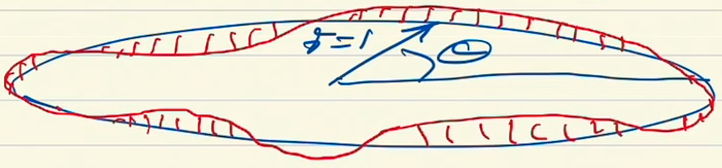
\includegraphics[scale=0.4]{methods3.png}
    \end{center}
	The \( z \) displacement of the wire produces the \( f(\theta) \) term.
	We wish to find \( \phi(r,\theta) \) for \( r < 1 \), assuming regularity at \( r = 0 \).
	Then, \( c_m = d_m = 0 \) and the solution is of the form
	\[
		\phi(r,\theta) = \frac{a_0}{2} + \sum_{m=1}^\infty \qty(a_m \cos m\theta + b_m \sin m\theta) r^m
	\]
	At \( r = 1 \),
	\[
		\phi(1,\theta) = f(\theta) = \frac{a_0}{2} + \sum_{m=1}^\infty \qty(a_m \cos m\theta + b_m \sin m\theta)
	\]
	which is exactly the Fourier series.
	Thus,
	\[
		a_m = \frac{1}{\pi} \int_0^{2\pi} f(\theta) \cos m \theta \dd{\theta};\quad b_m = \frac{1}{\pi} \int_0^{2\pi} f(\theta) \sin m \theta \dd{\theta}
	\]
	We can see from the equation that high harmonics are confined to have effects only near \( r = 1 \).
\end{example}

\subsection{Laplace's equation in cylindrical polar coordinates}
In cylindrical coordinates,
\[
	\laplacian \phi = \frac{1}{r} \pdv{r} \qty(r \pdv{\phi}{r}) + \frac{1}{4^2} \pdv[2]{\phi}{\theta} + \pdv[2]{\phi}{z} = 0
\]
With \( \phi = R(r) \Theta(\theta) Z(z) \), we find
\[
	\Theta'' = -\mu \Theta;\quad Z'' = \lambda Z;\quad r(rR')' + (\lambda r^2 - \mu) R = 0
\]
The polar equation can be easily solved by
\[
	\mu_m = m^2;\quad \Theta_m(\theta) = \cos m\theta, \sin m\theta
\]
The radial equation is Bessel's equation, giving solutions
\[
	R = J_m(kr), Y_m(kr)
\]
Setting boundary conditions in the usual way, defining \( R=0 \) at \( r = a \) means that
\[
	J_m(ka) = 0 \implies k = \frac{j_{mn}}{a}
\]
The radial solution is
\[
	R_{mn}(r) = J_m\qty(\frac{j_{mn}}{a}r)
\]
We have eliminated the \( Y_n \) term since we require \( r = 0 \) to give a finite \( \phi \).
Finally, the \( z \) equation gives
\[
	Z'' = k^2 Z \implies Z = e^{-kz}, e^{kz}
\]
We typically eliminate the \( e^{kz} \) mode due to boundary conditions, such as \( Z \to 0 \) as \( z \to \infty \).
The general solution is therefore
\[
	\phi(r,\theta,z) = \sum_{m=0}^\infty \sum_{n = 1}^\infty \qty(a_{mn} \cos m\theta + b_{mn} \sin m\theta) J_m\qty(\frac{j_{mn}}{a} r) e^{-\frac{j_{mn}r}{a}}
\]

\subsection{3D spherical polar coordinates}
In spherical polar coordinates,
\[
	\laplacian \Phi = \frac{1}{r^2} \pdv{r} \qty(r^2 \pdv{\Phi}{r}) + \frac{1}{r^2 \sin\theta}\pdv{\theta} \qty(\sin\theta \pdv{\Phi}{\theta}) + \frac{1}{r^2 \sin^2 \theta} \pdv[2]{\Phi}{\phi} = 0
\]
We will consider the \textit{axisymmetric case}; supposing that there is no \( \phi \) dependence.
We seek a separable solution of the form
\[
	\Phi(r,\theta) = R(r) \Theta(\theta)
\]
which gives
\[
	(\sin\theta \Theta')' + \lambda \sin\theta \Theta = 0;\quad (r^2R')' - \lambda R = 0
\]
Consider the substitution \( x = \cos\theta, \dv{x}{\theta} = -\sin\theta \) in the polar equation.
This gives \( \dv{\Theta}{\theta} = -\sin\theta \dv{\Theta}{x} \) and hence
\[
	-\sin\theta \dv{x}\qty[-\sin^2\theta \dv{\Theta}{x}] + \lambda \sin\theta \Theta = 0 \implies \dv{x}\qty[(1-x^2)\dv{\Theta}{x}] + \lambda \Theta = 0
\]
This gives Legendre's equation, so it has solutions of eigenvalues \( \lambda_\ell = \ell (\ell + 1) \) and eigenfunctions
\[
	\Theta_\ell(\theta) = P_\ell(x) = P_\ell(\cos\theta)
\]
The radial equation then gives
\[
	(r^2 R')' - \ell (\ell + 1) R = 0
\]
We will seek power law solutions: \( R = \alpha r^\beta \).
This gives
\[
	\beta(\beta + 1) - \ell(\ell + 1) = 0 \implies \beta = \ell, \beta = -\ell - 1
\]
Thus the radial eigenmodes are
\[
	R_\ell = r^{\ell}, r^{-\ell - 1}
\]
Therefore the general axisymmetric solution for spherical polar coordinates is
\[
	\Phi(r,\theta) = \sum_{\ell = 0}^\infty (a_\ell r^{\ell} + b_\ell r^{-\ell - 1}) P_\ell(\cos\theta)
\]
The \( a_\ell, b_\ell \) are determined by the boundary conditions.
Orthogonality conditions for the \( P_\ell \) can be used to determine coefficients.

Consider a solution to Laplace's equation on the unit sphere with axisymmetric boundary conditions given by
\[
	\Phi(1,\theta) = f(\theta)
\]
Given that we wish to find the interior solution, \( b_\ell = 0 \) by regularity.
Then,
\[
	f(\theta) = \sum_{\ell=0}^\infty a_\ell P_\ell(\cos\theta)
\]
By defining \( f(\theta) = F(\cos\theta) \),
\[
	F(x) = \sum_{\ell=0}^\infty a_\ell P_\ell(x)
\]
We can then find the coefficients in the usual way, giving
\[
	a_\ell = \frac{2\ell + 1}{2} \int_{-1}^1 F(x) P_{\ell}(x) \dd{x}
\]

\subsection{Generating function for Legendre polynomials}
Consider a charge at \( \bfr_0 = (x,y,z) = (0,0,1) \).
Then, the potential at a point \( P \) becomes
\begin{align*}
	\Phi(\bfr) & = \frac{1}{\abs{\bfr - \bfr_0}} = \frac{1}{(x^2 + y^2 + (x-1)^2)^{1/2}}                                         \\
	        & = \frac{1}{(r^2 (\sin^2 \phi + \cos^2 \phi) \sin^2 \theta + r^2 \cos^2 \theta - 2r \cos\theta + 1)^{1/2}} \\
	        & = \frac{1}{(r^2 \sin^2 \theta + r^2 \cos^2 \theta - 2r \cos\theta + 1)^{1/2}}                             \\
	        & = \frac{1}{(r^2 - 2r \cos\theta + 1)^{1/2}}                                                               \\
	        & = \frac{1}{(r^2 - 2r \overline x + 1)^{1/2}}
\end{align*}
where \( \overline x \equiv \cos \theta \).
This function \( \Phi \) is a solution to Laplace's equation where \( \bfr \neq \bfr_0 \).
Note that we can represent any axisymmetric solution as a sum of Legendre polynomials.
Now,
\[
	\frac{1}{\sqrt{r^2 - 2rx + 1}} = \sum_{\ell = 0}^\infty a_\ell P_\ell(x) r^\ell
\]
With the normalisation condition for the Legendre polynomials \( P_\ell(1) = 1 \), we find
\[
	\frac{1}{1-r} = \sum_{\ell=0}^\infty a_\ell r^\ell
\]
Using the geometric series expansion, we arrive at \( a_\ell = 1 \).
This gives
\[
	\frac{1}{\sqrt{r^2 - 2rx + 1}} = \sum_{\ell = 0}^\infty P_\ell(x) r^\ell
\]
which is the generating function for the Legendre polynomials.

\clearpage
\part{Inhomogeneous ODEs, Fourier Transforms}

\section{The Dirac Delta Function}
\subsection{Definition}\ \vspace*{-1.5em}
\begin{definition}
	We define a generalised function \( \delta(x - \xi) \) such that
	\begin{enumerate}[(i)]
		\item \( \delta(x-\xi) = 0 \) for all \( x \neq \xi \);
		\item \( \int_{-\infty}^\infty \delta(x-\xi) \dd{x} = 1 \).
	\end{enumerate}
	This acts as a linear operator \( \int \dd{x} \delta(x - \xi) \) on some function \( f(x) \) to produce a number \( f(\xi) \).
	\[
		\int_{-\infty}^\infty \dd{x} \delta(x-\xi) f(x) = f(\xi)
	\]
	This relationship holds provided that \( f(x) \) is sufficiently `well-behaved' at \( x=\xi \) and \( x\to\pm \infty \).
\end{definition}

\begin{remark}
	Strictly, the \( \delta \) `function' is classified as a distribution, not as a function.
	For this reason, we will never use \( \delta \) outside an integral, although such an integral may be implied.
	The \( \delta \) function represnts a unit point source or impulse.
\end{remark}

We can approximate the \( \delta \) function using a Gaussian approximation.
\[
	\delta_\varepsilon(x) = \frac{1}{\varepsilon \sqrt{\pi}} \exp[-\frac{x^2}{\varepsilon^2}]
\]
Therefore,
\begin{align*}
	\int_{-\infty}^\infty f(x) \delta(x) \dd{x} & = \lim_{\varepsilon \to 0} \int_{-\infty}^\infty \frac{1}{\varepsilon \sqrt{\pi}} \exp[-\frac{x^2}{\varepsilon^2}] f(x) \dd{x}            \\
	                                            & = \lim_{\varepsilon \to 0} \int_{-\infty}^\infty \frac{1}{\varepsilon \sqrt{\pi}} \exp[-y^2] f(\varepsilon y) \dd{y}                      \\
	                                            & = \lim_{\varepsilon \to 0} \int_{-\infty}^\infty \frac{1}{\varepsilon \sqrt{\pi}} \exp[-y^2] [f(0) + \varepsilon y f'(0) + \cdots] \dd{y} \\
	                                            & = f(0)
\end{align*}
for all well-behaved functions \( f \) at \( 0, \pm \infty \).
We could alternatively use the Dirichlet kernel
\[
	\delta_n(x) = \frac{\sin n x}{\pi x} = \frac{1}{2\pi} \int_{-n}^n e^{ikx} \dd{k}
\]
or even
\[
	\delta_n(x) = \frac{n}{2} \sech^2 nx
\]
\subsection{Properties of $\delta(x)$}
We define the Heaviside step function by
\[
	H(x) = \begin{cases}
		1 & x \geq 0 \\
		0 & x < 0
	\end{cases}
\]
For \( x \neq 0 \), we have
\[
	H(x) = \int_{-\infty}^x \delta(t) \dd{t}
\]
Thus,
\[
	\dv{x} H(x) = \delta(x)
\]
where this identification takes place under an implied integral.
We define \( \delta'(x) \) using integration by parts.
\begin{align*}
	\int_{-\infty}^\infty \delta'(x-\xi) f(x) \dd{x} & = \qty[\delta(x-\xi) f(x)]_{-\infty}^\infty - \int_{-\infty}^\infty \delta(x-\xi) f'(x) \dd{x} \\
	                                                 & = - \int_{-\infty}^\infty \delta(x-\xi) f'(x) \dd{x}                                           \\
	                                                 & = - f'(\xi)
\end{align*}
This is valid for all \( f \) that are smooth at \( x = \xi \).
\begin{example}
	Consider the Gaussian approximation:
	\[
		\delta_\varepsilon(x) = \frac{1}{\varepsilon \sqrt{\pi}} \exp[-\frac{x^2}{\varepsilon^2}]
	\]
	Then,
	\[
		\delta_\varepsilon'(x) = \frac{-2x}{\varepsilon^3 \sqrt{\pi}} \exp[-\frac{x^2}{\varepsilon^2}]
	\]
\end{example}

$ \delta(x) $ has the following properties: 

\paragraph{Sampling property} 
\[
    \int_{a}^{b} f(x) \delta(x - \xi) \,\mathrm{d}x = \begin{cases}
    f(\xi) &\text{if }a<\xi<b\\
    0 &\text{otherwise}\\
    \end{cases} 
\]

\paragraph{Even property}
\[
    \int_{-\infty}^{\infty} f(x) \delta(-(x-\xi)) \,\mathrm{d}x = \int_{-\infty}^{\infty} f(x) \delta(x-\xi) \,\mathrm{d}x
\]
This can be seen by change of variable $u = -(x-\xi)$. 

\paragraph{Scaling property}
\[
	\int_{-\infty}^\infty f(x) \delta(a(x-\xi)) \dd{x} = \frac{1}{\abs{a}}f(\xi)
\]

\paragraph{Advanced scaling} Let \( g(x) \) be a function with \( n \) isolated roots at \( x_1, \dots, x_n \).
Then, assuming \( g'(x) \) does not vanish at the \( x_i \),
\[
	\delta(g(x)) = \sum_{i=1}^n \frac{\delta(x - x_i)}{\abs{g'(x_i)}}
\]
This is a generalisation of the above.

\paragraph{Isolation property}
If \( g(x) \) is continuous at \( x = 0 \), then \( g(x) \delta(x) \) is equivalent to \( g(0) \delta(x) \) inside an integral.

\subsection{Fourier series expansion of delta function}

Consider a complex Fourier series expansion,
\[
	\delta(x) = \sum_{n=-\infty}^\infty c_n e^{in\pi x/L};\quad c_n = \frac{1}{2L}\int_{-L}^L \delta(x) e^{-i n \pi x / L} \dd{x} = \frac{1}{2L}
\]
Hence,
\[
	\delta(x) = \frac{1}{2L} \sum_{n=-\infty}^\infty e^{in\pi x/L}
\]
Let \( f(x) \) be a function, so \( f(x) = \sum_{n=-\infty}^\infty d_n e^{in \pi x / L} \).
Then, their inner product is given by
\[
	\int_{-L}^L f^*(x) \delta(x) \dd{x} = \frac{1}{2L} \sum_{n = -\infty}^\infty d_n \int_{-L}^L e^{-in \pi x/L} e^{in \pi x/L} \dd{x} = \sum_{n = -\infty}^\infty d_n = f(0)
\]
The Fourier expansion of the \( \delta \) function can be extended periodically to the whole real line.
This infinite set of \( \delta \) functions is known as the Dirac comb, given by
\[
	\sum_{m = -\infty}^\infty \delta(x-2mL) = \sum_{n = -\infty}^\infty e^{in \pi x/L}
\]

\subsection{Arbitrary eigenfunction expansion of delta function}
In general, suppose
\[
	\delta(x-\xi) = \sum_{n=1}^\infty a_n y_n(x)
\]
with coefficients
\[
	a_n = \frac{\int_a^b w(x) y_n(x) \delta(x-\xi) \dd{x}}{\int_a^b w(x) y_n(x)^2 \dd{x}} = \frac{w(\xi) y_n(\xi)}{\int_a^b w(x) y_n(x)^2 \dd{x}} = w_n(\xi) Y_n(\xi)
\]
Then,
\[
	\delta(x-\xi) = w(\xi) \sum_{n=1}^\infty Y_n(\xi) Y_n(x) = w(x) \sum_{n=1}^\infty Y_n(\xi) Y_n(x)
\]
since \( \frac{w(x)}{w(\xi)} \delta(x - \xi) = \delta(x - \xi) \).
Hence,
\[
	\delta(x-\xi) = w(x) \sum_{n=1}^\infty \frac{y_n(\xi) y_n(x)}{N_n}
\]
where \( N_n = \int_a^b w y_n^2 \dd{x} \) is a normalisation factor.
\begin{example}
	Consider a Fourier series for \( y(0) = y(1) = 0 \), with \( y_n(x) = \sin n \pi x \).
	From the sine series coefficient expression,
	\[
		\delta(x-\xi) = 2\sum_{n=1}^\infty \sin n \pi \xi \sin n \pi x
	\]
	where \( 0 < \xi < 1 \).
\end{example}

\section{Green's Functions}
\subsection{Motivation for Green's functions}
Consider a massive static string with tension \( T \) and linear mass density \( \mu \), suspended between fixed ends \( y(0) = y(1) = 0 \).
By resolving forces, we have the time independent form
\[
	T \dv[2]{y}{x} - \mu g = 0
\]
We will solve the inhomogeneous ODE \( - \dv[2]{y}{x} = f(x) \) with \( f(x) = -\frac{\mu g}{T} \).
This has been placed in Sturm-Liouville form.
We can integrate directly and find
\[
	-y = -\frac{\mu g}{2T} x^2 + k_1 x + k_2
\]
Imposing boundary conditions,
\[
	y(x) = \qty(-\frac{\mu g}{T}) \cdot \frac{1}{2}x(1-x)
\]
Consider alternatively a solution obtained by solving the equation for a single point mass \( \delta m = \mu \delta x \) suspended at \( x = \xi \) on an very light string.
We can then superimpose the solutions for each point mass to find the overall solution.
For a single point mass, the solution is given by two straight lines from \( (0,0) \) and \( (1,0) \) to the point mass \( (\xi_i, y_i(\xi_i)) \).
The angles of these straight lines from the horizontal are given by \( \theta_1, \theta_2 \).
Resolving in the \( y \) direction,
\begin{align*}
	0                                           & = T (\sin \theta_1 + \sin \theta_2) - \delta m g                \\
	                                            & = T\qty(\frac{-y_i}{\xi_i} + \frac{-y_i}{1-\xi_i}) - \delta m g \\
	\implies -T\qty(y_i(1-\xi_i) + y_i \xi_i) & = \delta m g \xi_i(1-\xi_i)                                     \\
	\implies y_i(\xi_i)                       & = \frac{-\delta m g}{T} \xi_i (1-\xi_i)
\end{align*}
So the solution is
\[
	y_i(x) = \frac{-\delta m g}{T} \begin{cases}
		x(1-\xi_i)    & x < \xi_i \\
		\xi_i (1 - x) & x > \xi_i
	\end{cases}
\]
which is the generalised sawtooth.
This can alternatively be written
\[
	f_i(\xi) G(x,\xi)
\]
where \( f_i \) is a source term, and \( G(x,\xi) \) is the Green's function, the solution for a unit point source.
Since the differential equation is linear, we can sum the solutions, giving
\[
	y(x) = \sum_{i=1}^N f_i(\xi) G(x, \xi_i)
\]
Taking a continuum limit,
\[
	f_i(\xi) = \frac{-\delta m g}{T} = \frac{-\mu \delta x g}{T} \equiv f(x) \dd{x} \implies f(x) = \frac{-\mu g}{T}
\]
which gives
\[
	y(x) = \int_0^1 f(\xi) G(x,\xi) \dd{\xi}
\]
Substituting the Green's function,
\begin{align*}
	y(x) & = \qty(\frac{-\mu g}{T}) \qty[ \int_0^x \xi(1-x) \dd{\xi} + \int_x^1 x(1-\xi) \dd{\xi}]              \\
	     & = \qty(\frac{-\mu g}{T}) \qty{ \qty[\frac{\xi^2}{2}(1-x)]_0^x + \qty[x(\xi - \frac{\xi^2}{2})]_x^1 } \\
	     & = \qty(\frac{-\mu g}{T}) \qty(\frac{x^2}{2}(1-x) - 0 + \frac{x}{2} - x\qty(x-\frac{x^2}{2}))         \\
	     & = \qty(\frac{-\mu g}{T}) \cdot \frac{1}{2}x(1-x)
\end{align*}
So we have found the correct solution in two ways; once by direct integration, and once by superimposing point solutions.
In general, direct integration is not trivial, and Green's functions are useful in this case.

\subsection{Definition of Green's function}
We wish to solve the inhomogeneous ODE
\[
	\mathcal L y \equiv \alpha(x) y'' + \beta(x) y' + \gamma(x) y = f(x)
\]
on \( a \leq x \leq b \), where \( \alpha \neq 0 \) and \( \alpha, \beta, \gamma \) are continuous and bounded, taking homogeneous boundary conditions \( y(a) = y(b) = 0 \).
\begin{definition}
    The Green's function for \( \mathcal L \) in this case is defined to be the solution for a unit point source at \( x = \xi \).
    That is, \( G(x,\xi) \) is the function that satisfies the boundary conditions and
    \[
        \mathcal L G(x,\xi) = \delta(x-\xi)
    \]
    so \( G(a,\xi) = G(b,\xi) = 0 \).
\end{definition}
Then, by linearity, the general solution is given by
\[
	y(x) = \int_a^b f(\xi) G(x,\xi) \dd{\xi}
\]
where \( y(x) \) satisfies the homogeneous boundary conditions.
We can verify this by checking
\[
	\mathcal L y = \int_a^b \mathcal L G(x,\xi) f(\xi) \dd{\xi} = \int_a^b \delta(x-\xi) f(\xi) \dd{\xi} = f(x)
\]
So the solution is given by the inverse operator
\[
	y = \mathcal L^{-1} f;\quad \mathcal L^{-1} = \int_a^b \dd{\xi} G(x,\xi)
\]
The Green's function spits into two parts;
\[
	G(x,\xi) = \begin{cases}
		G_1(x,\xi) & a \leq x < \xi \\
		G_2(x,\xi) & \xi < x < b
	\end{cases}
\]
For all \( x \neq \xi \), we have \( \mathcal L G_1 = \mathcal L G_2 = 0 \), so the parts are homogeneous solutions.
\( G \) satisfies the homogeneous boundary conditions, so \( G_1(a, \xi) = 0 \) and \( G_2(b, \xi) = 0 \).
\( G \) must be continuous at \( x = \xi \), hence \( G_1(\xi, \xi) = G_2(\xi, \xi) \).
There is a jump condition; the derivative of \( G \) is discontinuous at \( x = \xi \).
This satisfies
\[
	[G']_{\xi_-}^{\xi_+} = \eval{\dv{G_2}{x}}_{x = \xi_+} - \eval{\dv{G_1}{x}}_{x = \xi_-} = \frac{1}{\alpha(\xi)}
\]
where $ \alpha $ is defined in the original ODE above. 

\subsection{Explicit form for Green's functions}
We want to solve
\[
	\mathcal L G(x,\xi) = \delta(x-\xi)
\]
on \( a \leq x \leq b \), subject to homogeneous boundary conditions \( G(a,\xi) = G(b,\xi) = 0 \).
The functions \( G_1, G_2 \) satisfy the homogeneous equation, so \( \mathcal L G_i(x,\xi) = 0 \).
Suppose there exist two independent homogeneous solutions \( y_1(x), y_2(x) \) to \( \mathcal L y = 0 \).
Then, \( G_1 = A y_1 + B y_2 \), such that \( A y_1(a) + B y_2(a) = 0 \), which gives a constraint between \( A \) and \( B \).
This defines a complementary function \( y_-(x) \) such that \( y_-(a) = 0 \).
The general homogeneous solution with \( G_1(a) = 0 \) is
\[
	G_1 = C y_-
\]
\( C \) will be found later.
Similarly we can define \( y_+ \) as a linear combination of \( y_1, y_2 \) such that \( y_+(b) = 0 \).
\[
	G_2 = D y_+
\]
We require \( G_1(\xi, \xi) = G_2(\xi, \xi) \) for continuity, hence
\[
	C y_-(\xi) = D y_+(\xi)
\]
Since \( [G']_{\xi_-}^{\xi^+} = \frac{1}{\alpha(\xi)} \), we have
\[
	Dy'_+(\xi) - C Y_-'(\xi) = \frac{1}{\alpha(\xi)}
\]
We can solve these equations for \( C, D \) simultaneously to find
\[
	C(\xi) = \frac{y_+(\xi)}{\alpha(\xi)W(\xi)};\quad D(\xi) = \frac{y_-(\xi)}{\alpha(\xi)W(\xi)}
\]
where \( W(\xi) \) is the Wronskian
\[
	W(\xi) = y_-(\xi) y_+'(\xi) - y_+(\xi) y_-'(\xi)
\]
which is nonzero if \( y_-, y_+ \) are linearly independent.
Hence,
\[
	G(x,\xi) = \begin{cases}
		\dfrac{y_-(x) y_+(\xi)}{\alpha(\xi)W(\xi)} & a \leq x \leq \xi \\[1em]
		\dfrac{y_-(\xi) y_+(x)}{\alpha(\xi)W(\xi)} & \xi \leq x \leq b
	\end{cases}
\]

\subsection{Aside: Continuity of $G,G'$}
Why $G$ must be continuous at $\xi$ and have a jump discontinuity in its derivative?
\begin{proposition}
    $G$ is continuous at $x=\xi$. 
\end{proposition}
\begin{proof}
    Suppose $G$ is discontinuous at $\xi$. Then near $\xi$ we have 
    \[
        G \propto H(x-\xi) + \cdots 
    \]
    where $H$ is the Heaviside step function that will dominate as $x\to \xi$. Then $ G' \propto \delta(x-\xi) $ and $ G'' \propto \delta'(x-\xi) $, and the ODE becomes 
    \[
        \mathcal{L} G \propto \alpha \delta'(x-\xi) + \beta \delta(x-\xi) + \gamma H(x-\xi)
    \]
    But RHS there is no $ \delta' $ term, so contradiction. Hence $G$ must be continuous at $\xi$. 
\end{proof}

\begin{proposition}
    $G'$ has a jump discontinuity at $\xi$. 
\end{proposition}
\begin{proof}
    Integrate $ \mathcal{L} G(x,\xi)=\delta(x-\xi) $ across $ x=\xi $ by parts we get 
    \begin{align*}
        \text{LHS} &= \int_{\xi_-}^{\xi_+} \mathcal{L} G(x,\xi) \,\mathrm{d}x
        = \int_{\xi_-}^{\xi_+} \alpha G'' + \beta G' + \gamma G \,\mathrm{d}x
        = \cdots (\text{by parts}) \\
        &= \alpha(\xi) \qty[G']_{\xi_-}^{\xi_+} + (\beta-\alpha') \qty[G]_{\xi_-}^{\xi_+}  + 
        \int_{\xi_-}^{\xi_+} (\gamma-\beta'+\alpha'')G \,\mathrm{d}x\\ 
        &= \alpha(\xi) \qty[G']_{\xi_-}^{\xi_+}
    \end{align*}
    But RHS is 1, so we get 
    \[
         \qty[G']_{\xi_-}^{\xi_+} = \frac{1}{\alpha(\xi)}.\qedhere
    \]
\end{proof}

\subsection{Solving boundary value problems}
We know that the solution of \( \mathcal L y = f \) is
\[
	y(x) = \int_a^b G(x,\xi) f(\xi) \dd{\xi}
\]
We can split this into two intervals given that \( G = G_1 \) for \( \xi > x \) and \( G = G_2 \) for \( \xi < x \).
\begin{align*}
	y(x) & = \int_a^x G_2(x,\xi) f(\xi) \dd{\xi} + \int_x^b G_1(x,\xi) f(\xi) \dd{\xi}                                                               \\
	     & = y_+(x) \int_a^x \frac{y_-(\xi) f(\xi)}{\alpha(\xi)W(\xi)} \dd{\xi} + y_-(x) \int_a^x \frac{y_+(\xi) f(\xi)}{\alpha(\xi)W(\xi)} \dd{\xi}
\end{align*}
\begin{note}
    If \( \mathcal L \) is in Sturm-Liouville form, then \( \beta = \alpha' \), and the denominator \( \alpha(\xi)W(\xi) \) is a constant.

    Further, \( G \) is symmetric; \( G(x,\xi) = G(\xi,x) \).
Often, by convention, we take \( \alpha = 1 \) (however Sturm-Liouville form typically takes \( \alpha < 0 \)).

The indefinite integrals $ \int_{x} $ are particular integrals of solution. 
\end{note}

\begin{example}
	Consider \( y'' - y = f(x) \) with \( y(0) = y(1) = 0 \).
	Homogeneous solutions are \( y_1 = e^x \), \( y_2 = e^{-x} \).
	Imposing boundary conditions,
	\[
		G = \begin{cases}
			C \sinh x    & 0 \leq x < \xi \\
			D \sinh(1-x) & \xi < x \leq 1
		\end{cases}
	\]
	Continuity at \( x = \xi \) implies
	\[
		C \sinh \xi = D \sinh (1 - \xi) \implies C = D \frac{\sinh (1-\xi)}{\sinh \xi}
	\]
	The jump condition is
	\[
		-D \cosh(1-\xi) - C \cosh \xi = 1
	\]
	Substituting $C$ gives
	\begin{align*}
		-D\qty[\cosh(1-\xi)\sinh \xi + \sinh(1-\xi)\cosh \xi] & = \sinh \xi                     \\
		-D\qty[\sinh((1-\xi) + \xi)]                          & = \sinh \xi                     \\
		-D\sinh 1                                             & = \sinh \xi                     \\
		D                                                     & = \frac{\sinh \xi}{\sinh 1}     \\
		\implies C                                          & = \frac{-\sinh(1-\xi)}{\sinh 1}
	\end{align*}
	Therefore,
	\[
		y(x) = \frac{-\sinh(1-x)}{\sinh 1} \int_0^x \sinh \xi f(\xi) \dd{\xi} - \frac{\sinh x}{\sinh 1} \int_x^1 \sinh (1-\xi) f(\xi) \dd{\xi}
	\]
\end{example}

\paragraph{Inhomogeneous BCs}
Suppose we have inhomogeneous boundary conditions.
In this case, we want to find a homogeneous solution \( y_p \) that solves the inhomogeneous boundary conditions.

That is, \( \mathcal L y_p = 0 \) but \( y_p(a), y_p(b) \) are as required for the boundary conditions.

Then, by subtracting this solution from the original equation, we can solve using a homogeneous set of boundary conditions.
For instance, in the above example, suppose \( y(0) = 0, y(1) = 1 \).

We can find a solution \( y_p = \frac{\sinh x}{\sinh 1} \) which has the inhomogeneous boundary conditions but solves the homogeneous problem.

\subsection{Higher-order ODEs}
Suppose \( \mathcal L y = f(x) \) where \( \mathcal L \) is an \( n \)th order linear differential operator, and \( \alpha(x) \) is the coefficient for the highest degree derivative.
Suppose that homogeneous boundary conditions are satisfied.
Then we can define the Green's function in this case to be the function that solves
\[
	\mathcal L G(x,\xi) = \delta(x-\xi)
\]
which has the properties:
\begin{enumerate}
	\item \( G_1, G_2 \) are homogeneous solutions satisfying the homogeneous boundary conditions;
	\item \( G_1^{(k)}(\xi) = G_2^{(k)}(\xi) \) for \( k \in \qty{0, \dots, n-2} \);
	\item \( G_2^{(n-1)}(\xi^+) - G_1^{(n-1)}(\xi^-) = \frac{1}{\alpha(\xi)} \).
\end{enumerate}

\subsection{Eigenfunction expansions of Green's functions}
Suppose \( \mathcal L \) is in Sturm-Liouville form with eigenfunctions \( y_n(x) \) and eigenvalues \( \lambda_n \).
We seek \( G(x,\xi) = \sum_{n=1}^\infty A_n y_n(x) \) satisfying \( \mathcal L G = \delta(x-\xi) \).
\begin{align*}
	\mathcal L G & = \sum_n A_n \mathcal L y_n        \\
	             & = \sum_n A_n \lambda_n w(x) y_n(x)
\end{align*}
The \( \delta \) function has expansion
\[
	\delta(x-\xi) = w(x) \sum_n \frac{y_n(\xi) y_n(x)}{N_n};\quad N_n = \int w y_n^2 \dd{x}
\]
Hence,
\[
	A_n(\xi) = \frac{y_n(\xi)}{\lambda_n N_n}
\]
Thus,
\[
	G(x,\xi) = \sum_{n=1}^\infty \frac{y_n(\xi) y_n(x)}{\lambda_n \int w y_n^2 \dd{x}} = \sum_{n=1}^\infty \frac{Y_n(\xi) Y_N(x)}{\lambda_n}
\]
which was already obtained earlier in the course when studying Sturm-Liouville theory.

\subsection{Constructing Green's function for an initial value problem}
Suppose we want to solve \( \mathcal L y = f(t) \) for \( t \geq a \) with \( y(a) = y'(a) = 0 \), using \( G(t, \tau) \) satisfying \( \mathcal L g = \delta(t - \tau) \).

For \( t < \tau \), we have
\[
	G_1 = A y_1(t) + B y_2(t);\quad A y_1(a) + B y_2(a) = 0;\quad A y_1'(a) + B y_2'(a) = 0
\]
If \( A \neq B \neq 0 \), then we can solve this by dividing out \( A, B \) and find \( y_1 y_2' - y_2 y_1' = 0 \).
Since the Wronskian at \( a \) cannot be zero, \( A = B = 0 \).
So \( G_1(t,\tau) \equiv 0 \) for \( a \leq t < \tau \), so there is no change until the `impulse' at \( t = \tau \).

For \( t > \tau \), by continuity we must have \( G_2(\tau, \tau) = 0 \).
So we choose a complementary function \( G_2 = D y_+(t) \) with \( y_+(t) = A y_1(t) + B y_2(t) \), and \( y_+(\tau) = 0 \).

The discontinuity in the derivative implies that
\[
	G_2'(\tau, \tau) = Dy_+'(\tau) = \frac{1}{\alpha(\tau)}
\]
Hence,
\[
	A y_1'(\tau) + B y_2'(\tau) = \frac{1}{\alpha(\tau)} \implies D(\tau) = \frac{1}{\alpha(\tau) y_+'(\tau)}
\]
Hence we have a non-trivial solution
\[
	G(t, \tau) = \begin{cases}
		0                                      & t < \tau \\
		\dfrac{y_+(t)}{\alpha(\tau) y_+'(\tau)} & t > \tau
	\end{cases}
\]
The initial value problem has solution
\[
	y(t) = \int_a^t G_2(t, \tau) f(\tau) \dd{\tau} = \int_a^t \frac{y_+(t) f(\tau)}{y_+'(\tau)} \dd{\tau}
\]
Causality is `built in' to this solution.
Only forces which occur before \( t \) may have an impact on \( y(t) \).
\begin{example}
	Let us solve \( y''-y = f(t) \) with \( y(0) = y'(0) = 0 \).
	The homogeneous solution and initial conditions are
	\[
		t < \tau \implies G_1 \equiv 0
	\]
	and
	\[
		t > \tau \implies G_2 = A e^t + Be^{-t} = D \sinh (t - \tau)
	\]
	Now,
	\[
		[G']_{\tau_-}^{\tau_+} = \frac{1}{\alpha(\tau)} = 1 \implies G'(\tau, \tau) = D \cosh 0 = D = 1
	\]
	Hence, the solution is
	\[
		y(t) = \int_0^t f(\tau) \sinh (t - \tau) \dd{\tau}
	\]
\end{example}

\section{Fourier transform}
\subsection{Introduction}
Fourier transform is heavily used in solving complex ODEs, signal processing, etc. It transforms a linear ODE to an algebraic equation, which is easier to solve.
\begin{center}
\begin{tikzpicture}
	\draw (-5,3) rectangle (-2,2);
	\draw (-3.5,2.5) node[text width = 3cm, align=center]{Problem in transform space};
	\draw[->-=0.5] (-2,2.5) -- (2, 2.5);
	\draw (0, 2.5) node[anchor=south,text width = 2.5cm, align=center] {Relatively easy solution};
	\draw (2,2) rectangle (5,3);
	\draw (3.5,2.5) node [text width = 3cm, align=center]{Solution in transform space};
	\draw (-5,0) rectangle (-2,-1);
	\draw (-3.5,-0.5) node [text width = 3cm, align=center]{Original problem};
	\draw[->-=0.5] (-3.5, 0) -- (-3.5, 2) ;
	\draw (-3.5, 1) node[anchor=east,text width = 2.5cm, align=center] {Integral transform};
	\draw (2,0) rectangle (5,-1);
	\draw (3.5,-0.5) node[text width = 3cm, align=center] {Solution of original problem};
	\draw[dashed,->-=0.5] (-2,-0.5) -- (2,-0.5);
	\draw (0,-0.4) node[anchor=south,text width = 3cm, align=center] {Difficult solution};
	\draw[-<-=0.5] (3.5, 0) -- (3.5, 2) ;
	\draw (3.5,1) node[anchor=west,text width = 2.5cm, align=center] {Inverse transform};
\end{tikzpicture}
\end{center}
\begin{definition}
	The \textbf{Fourier transform} of a function \( f(x) \) is
	\[
		\widetilde f(k) = \mathcal F(f)(k) = \int_{-\infty}^\infty f(x) e^{-ikx} \dd{x}
	\]
	The \textbf{inverse Fourier transform} is
	\[
		f(x) = \mathcal F^{-1}\qty(\widetilde f)(x) = \frac{1}{2\pi} \int_{-\infty}^\infty \widetilde f(k) e^{ikx} \dd{k}
	\]
	Different internally-consistent definitions exist, which distribute the multiplicative constants in different ways.
\end{definition}
\begin{theorem}[Fourier inversion theorem]
	For a function \( f(x) \),
	\[
		\mathcal F^{-1} (\mathcal F (f))(x) = f(x)
	\]
	with a sufficient condition that \( f \) and \( \widetilde f \) are absolutely integrable, so
	\[
		\int_{-\infty}^\infty \abs{f(x)} \dd{x} = M < \infty
	\]
	In particular, \( f \to 0 \) as \( x \to \pm \infty \).
\end{theorem}


\begin{example}
	Consider the Gaussian,
	\[
		f(x) = \frac{1}{\sigma \sqrt{\pi}} \exp[-\frac{x^2}{\sigma^2}]
	\]
	We wish to compute its Fourier transform.
	Since \( i \sin kx \) is an odd function,
	\[
		\widetilde f(k) = \frac{1}{\sigma \sqrt{\pi}} \int_{-\infty}^\infty \exp[-\frac{x^2}{\sigma^2}] \exp[-ikx] \dd{x} = \frac{1}{\sigma \sqrt{\pi}} \int_{-\infty}^\infty \exp[-\frac{x^2}{\sigma^2}] \cos(kx) \dd{x}
	\]
	Consider, using Leibniz' rule,
	\[
		\dv{\widetilde f}{k} = \frac{-1}{\sigma \sqrt{\pi}} \int_{-\infty}^\infty x\exp[\frac{-x^2}{\sigma^2}] \sin kx \dd{x}
	\]
	Integrating by parts,
	\begin{align*}
		\dv{\widetilde f}{k} & = \frac{1}{\sigma \sqrt{\pi}} \qty[\frac{\sigma^2}{2} \exp[\frac{-x^2}{\sigma^2}] \sin kx]_{-\infty}^\infty - \frac{1}{\sigma \sqrt{\pi}} \int_{-\infty}^\infty \frac{k\sigma^2}{2} \exp[\frac{-x^2}{\sigma^2}] \cos kx \dd{x} \\
		                     & = \frac{1}{\sigma \sqrt{\pi}} \int_{-\infty}^\infty \frac{k\sigma^2}{2} \exp[\frac{-x^2}{\sigma^2}] \cos kx \dd{x}                                                                                                             \\
		                     & = -\frac{k\sigma^2}{2} \widetilde f(k)
	\end{align*}
	This is a differential equation for \( \widetilde f \), which gives
	\[
		\widetilde f(k) = C \exp[-\frac{k^2\sigma^2}{4}]
	\]
	Suppose \( k = 0 \).
	Then, in the original expression for the Fourier transform, we can directly find \( \widetilde f(0) = 1 \).
	Hence \( C \exp[-\frac{0^2\sigma^2}{4}] = 1 \implies C = 1 \).
	Hence,
	\[
		\widetilde f(k) = \exp[-\frac{k^2\sigma^2}{4}]
	\]
	which is another Gaussian with the width parameter inverted.
\end{example}
\begin{example}
    $ f(x) = e^{-a |x|} $ has Fourier transform $ \widetilde{f}(k) = 2a/(a^2+k^2) $. Note that
    \[
        f(x) = \begin{cases}
        e^{-ax} &x>0\\
        0 &x\le 0\\
        \end{cases} \implies \widetilde{f}(k) = \frac{1}{ik+a}. 
    \]
\end{example}

\subsection{Fourier transform and Fourier series}
Recall that the complex form of the Fourier series is
\[
	f(x) = \sum_{n=-\infty}^\infty c_n e^{ik_n x}
\]
where \( k_n = \frac{n\pi}{L} \).
We can write in particular \( k_n = n \Delta k \) where \( \Delta k = \frac{\pi}{L} \).
Then,
\[
	c_n = \frac{1}{2L} \int_{-L}^L f(x) e^{-ik_n x} \dd{x} = \frac{\Delta k}{2\pi} \int_{-L}^L f(x) e^{-ik_n x}\dd{x}
\]
Now, re-substituting into the Fourier series,
\[
	f(x) = \sum_{n=-\infty}^\infty \frac{\Delta k}{2\pi} e^{i k_n x} \int_{-L}^L f(x') e^{-ik_n x'} \dd{x'}
\]
Interpreting the sum multiplied by \( \Delta k \) as a Riemann integral,
\[
	f(x) \to \int_{-\infty}^\infty \frac{1}{2\pi} e^{i k x} \int_{-L}^L f(x') e^{-ik x'} \dd{x'} \dd{k}
\]
Taking the limit \( L \to \infty \),
\[
	f(x) = \frac{1}{2\pi} \int_{-\infty}^\infty \dd{k} e^{i k x} \int_{-\infty}^\infty \dd{x'} f(x') e^{-ik x'}
\]
which is the inverse Fourier transform of the Fourier transform of \( f \), which gives the Fourier inversion theorem.
Note that when \( f(x) \) is discontinuous at \( x \), the Fourier transform gives
\[
	\mathcal F^{-1}(\mathcal F(f))(x) = \frac{1}{2}(f(x_-) + f(x_+))
\]
which is analogous to the result for Fourier series.

\subsection{Properties of Fourier transforms}
Recall the definition of the Fourier transform.
\[
	\widetilde f(k) = \int_{-\infty}^\infty f(x) e^{-ikx} \dd{x}
\]
\paragraph{Linearity} The (inverse) Fourier transform is linear.
\[
	h(x) = \lambda f(x) + \mu g(x) \iff \widetilde h(k) = \lambda \widetilde f(k) + \mu \widetilde g(k)
\]

\paragraph{Translation} Translated functions transform to multiplicative factors.
\[
	h(x) = f(x - \lambda) \iff \widetilde h(k) = e^{-i\lambda k} \widetilde f(k)
\]
This is because
\[
	\widetilde h(k) = \int f(x - \lambda) e^{-ikx} \dd{x} = \int f(y) e^{-ik(y + \lambda)} \dd{y} = e^{-i\lambda k} \widetilde f(k)
\]

\paragraph{Frequency shift} Frequency shifts transform to translations in frequency space.
\[
	h(x) = e^{i\lambda x}f(x) \implies \widetilde h(k) = \widetilde f(k - \lambda)
\]

\paragraph{Scaling} A scalar multiple applied to the argument transforms into an inverse scalar multiple.
\[
	h(x) = f(\lambda x) \iff \widetilde h(k) = \frac{1}{\abs{\lambda}} \widetilde f\qty(\frac{k}{\lambda})
\]

\paragraph{Multiplication by $x$} Multiplication by \( x \) transforms into an imaginary derivative.
\[
	h(x) = xf(x) \iff \widetilde h(k) = i\widetilde f'(k)
\]
This is because
\[
	\int_{-\infty}^\infty xf(x) e^{-ikx} \dd{x} = \frac{-1}{i} \dv{k} \int_{-\infty}^\infty f(x) e^{-ikx} \dd{x}
\]

\paragraph{Derivative} Derivatives transform into a muliplication by \( ik \).
\[
	h(x) = f'(x) \iff \widetilde h(k) = ik \widetilde f(k)
\]
This is because we can integrate by parts and find
\[
	\widetilde h(k) = \int_{-\infty}^\infty f'(x) e^{-ikx} \dd{x} = \underbrace{\qty[f(x) e^{-ikx}]_{-\infty}^\infty}_{=0} + ik\int_{-\infty}^\infty f(x) e^{-ikx} \dd{x}
\]

\paragraph{General duality} The \textit{general duality} property states that by mapping \( x \mapsto -x \), we have
\[
	f(-x) = \frac{1}{2\pi} \int_{-\infty}^\infty \widetilde f(k) e^{-ikx} \dd{k}
\]
hence mapping \( k \leftrightarrow x \), treating \( \widetilde f \) now as a function in position space, we have
\[
	f(-k) = \frac{1}{2\pi} \int_{-\infty}^\infty \widetilde f(x) e^{-ikx} \dd{x}
\]
Thus
\[
	g(x) = \widetilde f(x) \iff \widetilde g(k) = 2\pi f(-k)
\]
We can then write the corollary that
\[
	f(-x) = \frac{1}{2\pi} \mathcal F(\mathcal F(f))(x)
\]
Finally,
\[
	\mathcal F^4(f)(x) = 4\pi^2 f(x)
\]

\begin{example}[Top hat]
	Consider a function defined by
	\[
		f(x) = \begin{cases}
			1 & \abs{x} \leq a   \\
			0 & \text{otherwise}
		\end{cases}
	\]
	for some \( a > 0 \).
	By the definition of the Fourier transform,
	\[
		\widetilde f(k) = \int_{-\infty}^\infty f(x) e^{-ikx} \dd{x} = \int_{-a}^a e^{-ikx} \dd{x} = \int_{-a}^a \cos kx \dd{x} = \frac{2}{k} \sin ka
	\]
	By the Fourier inversion theorem,
	\[
		\frac{1}{\pi} \int_{-\infty}^\infty e^{ikx} \frac{1}{k} \sin ka \dd{k} = f(x)
	\]
	for \( x \neq a \).
	Now, in this expression, let \( x = 0 \) and let \( k \mapsto x \).
	We arrive at the Dirichlet discontinuous formula.
	\[
		\int_0^\infty \frac{\sin ax}{x} \dd{x} = \frac{\pi}{2} \sgn a = \begin{cases}
			\frac{\pi}{2}  & a > 0 \\
			0              & a = 0 \\
			-\frac{\pi}{2} & a < 0
		\end{cases}
	\]
\end{example}

\subsection{Convolution}
We want to multiply Fourier transforms in the frequency domain (transformed space).
This is useful for filtering or processing signals.
\[
	\widetilde h(k) = \widetilde f(k) \widetilde g(k)
\]
Consider the inverse.
\begin{align*}
	h(x) & = \frac{1}{2\pi} \int_{-\infty}^\infty \widetilde f(k) \widetilde g(k) e^{ikx} \dd{k}                                    \\
	     & = \frac{1}{2\pi} \int_{-\infty}^\infty \qty(\int_{-\infty}^\infty f(y) e^{-iky} \dd{y}) \widetilde g(k) e^{ikx} \dd{k}   \\
	     & = \int_{-\infty}^\infty f(y) \qty( \frac{1}{2\pi} \int_{-\infty}^\infty e^{-iky} \widetilde g(k) e^{ikx} \dd{k} ) \dd{y} \\
	     & = \int_{-\infty}^\infty f(y) \qty( \frac{1}{2\pi} \int_{-\infty}^\infty \widetilde g(k) e^{ik(x-y)} \dd{k} ) \dd{y}      \\
	     & = \int_{-\infty}^\infty f(y) g(x-y) \dd{y}                                                                               \\
	     & = (f \ast g)(x)
\end{align*}
where \( f \ast g \) is called the \textbf{convolution} of \( f \) and \( g \).
By duality, we also have
\[
	h(x) = f(x) g(x) \implies \widetilde h(k) = \frac{1}{2\pi} \int_{-\infty}^\infty \widetilde f(p) \widetilde g(k-p) \dd{p} = \frac{1}{2\pi}\qty(\widetilde f \ast \widetilde g)(k)
\]

\subsection{Parseval's theorem}
Consider \( h(x) = g^*(-x) \).
Then, by letting \( x = -y \),
\begin{align*}
	\widetilde h(k) & = \int_{-\infty}^\infty g^*(-x) e^{-ikx} \dd{x}      \\
	                & = \qty[\int_{-\infty}^\infty g(-x) e^{ikx} \dd{x}]^* \\
	                & = \qty[\int_{-\infty}^\infty g(y) e^{-iky} \dd{y}]^* \\
	                & = \widetilde g^*(k)
\end{align*}
Substituting this into the convolution theorem, with \( g(x) \mapsto g^*(-x) \), we have
\[
	\int_{-\infty}^\infty f(y) g^*(y-x) \dd{y} = \frac{1}{2\pi} \int_{-\infty}^\infty \widetilde f(k) \widetilde g^*(k) e^{ikx} \dd{x}
\]
Taking \( x = 0 \) in this expression and mapping \( y \mapsto x \), we find
\[
	\int_{-\infty}^\infty f(x) g^*(x) \dd{x} = \frac{1}{2\pi} \int_{-\infty}^\infty \widetilde f(k) \widetilde g^*(k) \dd{x}
\]
Equivalently,
\[
	\inner{g,f} = \frac{1}{2\pi} \inner{\widetilde g, \widetilde f}
\]
So the inner product is conserved under the Fourier transform (up to a factor of \( 2 \pi \)).
Now, by setting \( g^* = f^* \), we have
\[
	\int_{-\infty}^\infty \abs{f(x)}^2 \dd{x} = \frac{1}{2\pi} \int_{-\infty}^\infty \abs{\widetilde f(k)}^2 \dd{k}
\]
This is Parseval's theorem.

\subsection{Fourier transforms of generalised functions}
\paragraph*{Dirac delta function.}
We can apply Fourier transforms to generalised functions by considering limiting distributions.
Consider the inversion
\begin{align*}
	f(x) & = \mathcal F^{-1}(\mathcal F(f))(x)                                                                                                          \\
	     & = \frac{1}{2\pi} \int_{-\infty}^\infty \qty[\int_{-\infty}^\infty f(u) e^{-iku} \dd{u}] e^{ikx} \dd{k}                                       \\
	     & =\int_{-\infty}^\infty f(u) \underbrace{\qty[\frac{1}{2\pi} \int_{-\infty}^\infty e^{-ik(x-u)} \dd{k}]}_{\delta(x-u)} \dd{u}
\end{align*}
In order to reconstruct \( f(x) \) on the right hand side for any function \( f \), we must have that the bracketed term is \( \delta(x-u) \).
So we identify
\[
	\delta(x-u) = \frac{1}{2\pi} \int_{-\infty}^\infty e^{ik(x-u)} \dd{k}
\]
If \( f(x) = \delta(x) \),
\[
	\widetilde f(k) = \int_{-\infty}^\infty \delta(x) e^{ikx} \dd{x} = 1
\]
This can be thought of as the Fourier transform of an infinitely thin Gaussian, which becomes an infinitely wide Gaussian (a constant).

If \( f(x) = 1 \), then
\[
	\widetilde f(k) = \int_{-\infty}^\infty e^{-ikx}\dd{x} = 2\pi \delta(k)
\]
This can also be found by the duality formula.

If \( f(x) = \delta(x - a) \), we have
\[
	\widetilde f(k) = e^{-ika}
\]
This is a translation of the original Fourier transform for the \( \delta \) function above.

\paragraph{Trigonometric functions.}
Let \( f(x) = \cos \omega x = \frac{1}{2} \qty(e^{ix} + e^{-ix}) \).
Then,
\[
	\widetilde f(k) = \pi\qty(\delta(k+\omega) + \delta(k-\omega))
\]
For \( f(x) = \sin \omega x \), we have
\[
	\widetilde f(k) = i\pi\qty(\delta(k+\omega) - \delta(k-\omega))
\]
Using duality,
\begin{align*}
	f(x) & = \frac{1}{2}\qty(\delta(x+a) + \delta(x-a)) \implies \widetilde f(k) = \cos ka  \\
	f(x) & = \frac{1}{2i}\qty(\delta(x+a) - \delta(x-a)) \implies \widetilde f(k) = \sin ka
\end{align*}

\paragraph{Heaviside functions.}
Let \( H(x) \) be the Heaviside function, such that \( H(0) = \frac{1}{2} \).
Then, \( H(x) + H(-x) = 1 \) for all \( x \).
We can take the Fourier transform of this and find
\[
	\widetilde H(k) + \widetilde H(-k) = 2\pi \delta(k)
\]
Recall that \( H'(x) = \delta(x) \).
Thus,
\[
	ik \widetilde H(x) = \widetilde \delta(k) = 1
\]
Since \( k \delta(k) = 0 \), the two equations for \( \widetilde H \) can be consistent if we take
\[
	\widetilde H(k) = \pi\delta(k) + \frac{1}{ik}
\]

\paragraph{Dirichlet discontinuous formula.}
Recall the Dirichlet discontinuous formula:
\[
	\int_0^\infty \frac{\sin ax}{x} \dd{x} = \frac{\pi}{2} \sgn a = \begin{cases}
		\frac{\pi}{2}  & a > 0 \\
		0              & a = 0 \\
		-\frac{\pi}{2} & a < 0
	\end{cases}
\]
We can rewrite this as
\[
	\frac{1}{2} \sgn x = \frac{1}{2\pi} \int_{-\infty}^\infty \frac{e^{ikx}}{ik} \dd{k}
\]
since the cosine term divided by \( ik \) is odd.
Hence,
\[
	f(x) = \frac{1}{2} \sgn x \iff \widetilde f(k) = \frac{1}{ik}
\]
This is the preferred form for a Heaviside-type function when used in Fourier transforms.

\subsection{Solving ODEs for boundary value problems}
Consider \( y'' - y = f(x) \) with homogeneous boundary conditions \( y \to 0 \) as \( x \to \pm \infty \).
Taking the Fourier transform of this expression, we find
\[
	(-k^2 - 1) \widetilde y = \widetilde f
\]
Thus, the solution is
\[
	\widetilde y(k) = \frac{-\widetilde f(k)}{1+k^2} \equiv \widetilde f(k) \widetilde g(k)
\]
where \( \widetilde g(k) = \frac{-1}{1 + k^2} \).
Note that \( \widetilde g(k) \) is the Fourier transform of \( g(x) = -\frac{1}{2} e^{-\abs{x}} \).
Applying the convolution theorem,
\begin{align*}
	y(x) & = \int_{-\infty}^\infty f(u) g(x-u) \dd{u}                                                    \\
	     & = -\frac{1}{2} \int_{-\infty}^\infty f(u) e^{-\abs{x-u}}\dd{u}                                \\
	     & = -\frac{1}{2} \qty[ \int_{-\infty}^x f(u) e^{u-x}\dd{u} + \int_x^\infty f(u) e^{x-u}\dd{u} ]
\end{align*}
This is in the form of a boundary value problem Green's function.
We can construct the same results by constructing the Green's function directly.

\subsection{Signal processing}
Suppose we have an input signal \( \mathcal I(t) \), which is acted on by some linear operator \( \mathcal L_{\text{in}} \) to yield an output \( \mathcal O(t) \).
The Fourier transform of the input \( \widetilde{\mathcal I}(\omega) \) is called the \textbf{resolution}.
\[
	\widetilde{\mathcal I}(\omega) = \int_{-\infty}^\infty \mathcal I(t) e^{-i\omega t} \dd{t}
\]
In the frequency domain, the action of \( \mathcal L_{\text{in}} \) on \( \mathcal I(t) \) means that \( \widetilde{\mathcal I}(\omega) \) is multiplied by a transfer function \( \widetilde{\mathcal R}(\omega) \).
Thus,
\[
	\mathcal O(t) = \frac{1}{2\pi} \int_{-\infty}^\infty \widetilde{\mathcal R}(\omega) \widetilde{\mathcal I}(\omega) e^{i\omega t} \dd{\omega}
\]
The inverse Fourier transform of the transfer function, \( \mathcal R \), is called the \textbf{response function}, which is given by
\[
	\mathcal R(t) = \frac{1}{2\pi} \int_{-\infty}^\infty \widetilde{\mathcal R}(\omega) e^{i \omega t}\dd{\omega}
\]
By the convolution theorem,
\[
	\mathcal O(t) = \int_{-\infty}^\infty \mathcal I(u) \mathcal R(t-u) \dd{u}
\]
Suppose there is no input (\( \mathcal I(t) = 0 \)) for \( t < 0 \).
By causality, there should be zero output for the response function (\( \mathcal R(t) = 0 \)) for \( t < 0 \).
Therefore, we require \( 0 < u < t \) and hence
\[
	\mathcal O(t) = \int_0^t \mathcal I(u) \mathcal R(t-u) \dd{u}
\]
which resembles an initial value problem Green's function.

\subsection{General transfer functions for ODEs}
Suppose an input-output relationship is given by a linear ODE.\@
\[
	\mathcal L \mathcal O(t) \equiv \qty(\sum_{i=0}^n a_i \dv[i]{x}) \mathcal O(t) \equiv \mathcal I(t)
\]
Here, \( \mathcal L_{\text{in}} = 1 \).
We want to solve this ODE using a Fourier transform.
\[
	(a_0 + a_1 i\omega - a_2 \omega^2 - a_3 i\omega^3 + \dots + a_n (i \omega)^n) \widetilde{\mathcal O}(\omega) = \widetilde{\mathcal I}(\omega)
\]
We can solve this algebraically in Fourier transform space.
The transfer function is
\[
	\widetilde{\mathcal R}(\omega) = \frac{1}{a_0 + \dots + a_n (i \omega)^n}
\]
We factorise the denominator to find partial fractions.
Suppose there are \( J \) distinct roots \( (i \omega - c_j)^{k_j} \), where \( k_j \) is the algebraic multiplicity of the \( j \)th root, so \( \sum_{j=1}^J k_j = n \).
So we can write
\[
	\widetilde{\mathcal R}(\omega) = \frac{1}{(i \omega - c_1)^{k_1} \dots (i \omega - c_J)^{k_J}}
\]
Expressing this as partial fractions,
\[
	\widetilde{\mathcal R}(\omega) = \sum_{j=1}^J \sum_{m=1}^{k_i} \frac{\Gamma_{jm}}{(i\omega - c_j)^m}
\]
The \( \Gamma_{jm} \) terms are constant.
To solve this, we must find the inverse Fourier transform of \( (i\omega - a)^{-m} \).
Recall that
\[
	\mathcal F^{-1}\qty(\frac{1}{i\omega - a}) = \begin{cases}
		e^{at} & t > 0 \\
		0      & t < 0
	\end{cases}
\]
for \( \Re a < 0 \).
So we will require \( \Re c_j < 0 \) for all \( j \) to eliminate exponentially growing solutions.
Note that for \( n = 2 \),
\[
	i \dv{\omega} \qty(\frac{1}{i \omega - a}) = \frac{1}{(i \omega-a)^2}
\]
and recall that
\[
	\mathcal F (t f(t)) = i \widetilde{f}'(\omega)
\]
Hence,
\[
	\mathcal F^{-1}\qty(\frac{1}{(i \omega - a)^2}) = \begin{cases}
		t e^{at} & t > 0 \\
		0        & t < 0
	\end{cases}
\]
Inductively, we arrive at
\[
	\mathcal F^{-1}\qty(\frac{1}{(i \omega - a)^m}) = \begin{cases}
		\frac{t^{m-1}}{(m-1)!} e^{at} & t > 0 \\
		0                             & t < 0
	\end{cases}
\]
We can therefore invert any transfer function to obtain the response function.
Thus the response function takes the form
\[
	\mathcal R(t) = \sum_{j=1}^J \sum_{m=1}^{k_i} \Gamma_{jm} \frac{t^{m-1}}{(m-1)!} e^{c_j t};\quad t > 0
\]
and zero for \( t < 0 \).
We can now solve such differential equations in Green's function form, or directly invert \( \widetilde{\mathcal R}(\omega) \widetilde{\mathcal I}(\omega) \) for a polynomial \( \widetilde{\mathcal I}(\omega) \).

\begin{example}[Damped oscillator]
	We can use the Fourier transform method to solve the differential equation
\[
	\mathcal L y \equiv y'' + 2py' + (p^2 + q^2)y = f(t)
\]
where \( p > 0 \).
Consider homogeneous boundary conditions \( y(0) = y'(0) = 0 \).
The Fourier transform is
\[
	(i\omega)^2 \widetilde y + 2 i p \omega \widetilde y + (p^2 + q^2) \widetilde y = \widetilde f
\]
Hence,
\[
	\widetilde y = \frac{\widetilde f}{-\omega^2 + 2ip\omega + p^2 + q^2} \equiv \widetilde R \widetilde f
\]
We can invert this using the convolution theorem by inverting \( \widetilde R \).
\[
	y(t) = \int_0^t \mathcal R(t-\tau) f(\tau) \dd{\tau}
\]
where the response function is
\[
	\mathcal R(t - \tau) = \frac{1}{2\pi} \int_{-\infty}^\infty \frac{e^{i\omega(t-\tau)}}{p^2 + q^2 + 2ip\omega - \omega^2} \dd{\omega}
\]
We can show that \( \mathcal L \mathcal R(t-\tau) = \delta(t-\tau) \); in other words, \( \mathcal R \) is the Green's function.
\end{example}

\subsection{Discrete Fourier transform}
\subsubsection{Discrete sampling and the Nyquist frequency}
Suppose a signal \( h(t) \) is sampled at equal times \( t_n = n\Delta \) with a time step \( \Delta \) and values \( h_n = h(t_n) = h(n\Delta) \), for all \( n \in \mathbb Z \).
The sampling frequency is therefore \( \Delta^{-1} \), so the sampling angular velocity is \( \omega_s = 2\pi f_s = \frac{2\pi}{\Delta} \).
\begin{definition}
	The \textbf{Nyquist frequency} is \( f_c = \frac{1}{2\Delta} \), which is the highest frequency actually sampled at \( \Delta \).
\end{definition}
Suppose we have a signal \( g_f \) with a given frequency \( f \).
We will write
\[
	g_f(t) = A \cos(2\pi f t + \varphi) = \Re \qty(A e^{2 \pi i f t + \varphi}) = \frac{1}{2} \qty(A e^{2 \pi i f t + \varphi}) + \frac{1}{2} \qty(A e^{-2 \pi i f t + \varphi})
\]
where \( A \in \mathbb R \).
Note that this signal has two `frequencies'; a positive and a negative frequency.
The combination of these frequencies gives the full wave.

Suppose we sample \( g_f(t) \) at the Nyquist frequency, so \( f = f_c \).
Then,
\begin{align*}
	g_{f_c}(t_n) & = A \cos(2 \pi \frac{1}{2\Delta} n \Delta + \varphi) \\
	             & = A \cos(\pi n + \varphi)                            \\
	             & = A \cos \pi n \cos \phi + A \sin \pi n \sin \phi    \\
	             & = A' \cos(2\pi f_c t_n)
\end{align*}
where \( A' = A \cos \phi \).
This has removed half of the information about the wave; the ampliude and the phase have become degenerate.

We can identify \( f_c \) with \( -f_c \) when considering the remaining information; we say that the two frequencies are \textit{aliased} together.
Now, suppose we sample at greater than the Nyquist frequency, in particular \( f = f_c + \delta f > f_c \), where for simplicity we let \( \delta f < f_c \).
We have
\begin{align*}
	g_f(t_n) & = A \cos(2\pi (f_c + \delta f)t_n + \varphi) \\
	         & = A \cos(2\pi (f_c - \delta f)t_n - \varphi)
\end{align*}
So frequencies above the Nyquist frequency are reinterpreted after the sampling as a frequency lower than the Nyquist frequency.
This aliases \( f_c + \delta f \) with a ``ghost signal'' \( f_c - \delta f \) (actually $ -(f_c-\delta f) $).

\subsubsection{Nyquist-Shannon sampling theorem}
In order to avoid this aliase effect, we are going to put \textit{bandwidth} limit to our signal, which eliminates the effect. 
\begin{definition}
	A signal \( g(t) \) is \textbf{bandwidth-limited} if it contains no frequencies above \( \omega_{\max} = 2\pi f_{\max} \).
	In other words, \( \widetilde g(\omega) = 0 \) for all \( \abs{\omega} > \omega_{\max} \).
	In this case,
	\[
		g(t) = \frac{1}{2\pi} \int_{-\infty}^\infty \widetilde g(\omega) e^{i\omega t} \dd{\omega} = \frac{1}{2\pi} \int_{-\omega_{\max}}^{\omega_{\max}} \widetilde g(\omega) e^{i\omega t} \dd{\omega}.
	\]
\end{definition}
\noindent Suppose we set the sampling rate to the Nyquist frequency, i.e. \( \Delta = \frac{1}{2f_{\max}} \).
Then,
\[
	g_n \equiv g(t_n) = \frac{1}{2\pi} \int_{-\omega_{\max}}^{\omega_{\max}} \widetilde g(\omega) e^{i\pi n \omega / \omega_{\max}} \dd{\omega}
\]
This is a complex Fourier series coefficient \( c_n \), multiplied by \( \frac{\omega_{\max}}{\pi} \).
The Fourier series is periodic in \( \omega \) with period \( 2 \omega_{\max} \), not in space or time.
\[
	\widetilde g_\mathrm{per}(\omega) = \frac{\pi}{\omega_{\max}} \sum_{n=-\infty}^\infty g_n e^{-i \pi n \omega / \omega_{\max}}
\]
The actual Fourier transform \( \widetilde g \) is found by multiplying by a top hat window function
\[
	\widetilde h(\omega) = \begin{cases}
		1 & \abs{\omega} \leq \omega_{\max} \\
		0 & \text{otherwise}
	\end{cases}
\]
Hence,
\[
	\widetilde g(\omega) = \widetilde g_\mathrm{per}(\omega) \widetilde h(\omega)
\]
Note that this relation is exact.
Inverting this expression,
\begin{align*}
	g(t) & = \frac{1}{2\pi} \int_{-\infty}^\infty \widetilde g_\mathrm{per}(\omega) \widetilde h(\omega) e^{i \omega t} \dd{\omega}                                     \\
	     & = \frac{1}{2\omega_{\max}} \sum_{n=-\infty}^\infty g_n \int_{-\omega_{\max}}^{\omega_{\max}} \exp(i \omega\qty(t - \frac{n \pi}{\omega_{\max}})) \dd{\omega}
\end{align*}
Only the cosine term is even, hence
\[
	g(t) = \frac{1}{2\omega_{\max}} \sum_{n=-\infty}^\infty g_n \frac{\sin(\omega_{\max} t - \pi n)}{\omega_{\max} t - \pi n}
\]
Hence, \( g(t) \) can be written \textit{exactly} as a combination of countably many discrete sample points.

\subsubsection{Discrete Fourier transform}
Suppose we have a finite number of samples \( h_m = h(t_m) \) for \( t_m = m \Delta \), where \( m = 0,\dots, N-1 \).
We will approximate the Fourier transform for \( N \) frequencies within the Nyquist frequency \( f_c = \frac{1}{2\Delta} \), using equally-spaced frequencies, given by \( \Delta_f = \frac{1}{N\Delta} \) in the range \( -f_c \leq f \leq f_c \).

We could take the convention \( f_n = n \Delta_f = \frac{n}{N\Delta} \) for \( n = -\frac{N}{2}, \dots, \frac{N}{2} \).
However, this overcounts the Nyquist frequency (which is aliased), giving \( N + 1 \) frequencies instead of the desired \( N \).
Since frequencies above the Nyquist frequency are aliased to below it:
\[
	\qty(\frac{N}{2} + m) \Delta f = f_c + \delta f \mapsto \qty(\frac{N}{2} - m)\Delta f = -(f_c - \delta f)
\]
we can instead use the convention \( f_n = n \Delta_f = \frac{n}{N\Delta} \) for \( n = 0, \dots, N - 1 \).
This counts the Nyquist frequency only once.
The Fourier transform at a frequency \( f_n \) becomes
\begin{align*}
	\widetilde h(f_n) & = \int_{-\infty}^\infty h(t) e^{-2\pi if_n t} \dd{t}    \\
	                  & \approx \Delta \sum_{m=0}^{N-1} h_m e^{-2\pi i f_n t_m} \\
	                  & = \Delta \sum_{m=0}^{N-1} h_m e^{-2\pi i m n / N}       \\
	                  & = \Delta \widetilde h_d(f_n)
\end{align*}
where the function \( \widetilde h_d(f_n) \) is the \textbf{discrete Fourier transform}.
The matrix 
\[
	[\mathrm{DFT}]_{mn} = e^{-2\pi i m n / N}
\]
defines the discrete Fourier transform for the vector \( \bfh = \qty{h_m} \).
The discrete Fourier transform is then
\[
	\widetilde \bfh_d = [\mathrm{DFT}] \bfh
\]
By inverting the discrete Fourier transform matrix, we find
\[
	\bfh = [\mathrm{DFT}]^{-1} \widetilde \bfh_d = \frac{1}{N} [\mathrm{DFT}]^\dagger \widetilde \bfh_d
\]
since the inverse of the discrete Fourier transform matrix is its adjoint.
The matrix is built from roots of unity \( \omega = e^{-2\pi i/N} \).
So, for instance, \( n = 4 \) gives \( \omega = e^{-2\pi i/4} = -i \) giving
\[
	[\mathrm{DFT}] = \begin{pmatrix}
		1 & 1  & 1  & 1  \\
		1 & -i & -1 & i  \\
		1 & -1 & 1  & -1 \\
		1 & i  & -1 & -i
	\end{pmatrix}
\]
The inverse discrete Fourier transform is
\begin{align*}
	h_m & = h(t_m)                                                                                  \\
	    & = \frac{1}{2\pi} \int_{-\infty}^\infty \widetilde h(\omega) e^{i \omega t_m} \dd{\omega}  \\
	    & = \int_{-\infty}^\infty \widetilde h(f) e^{2\pi i f t_m} \dd{f}                           \\
	    & \approx \frac{1}{\Delta N} \sum_{n=0}^{N-1} \Delta \widetilde h_d(f_n) e^{2\pi i m n / N} \\
	    & = \frac{1}{N} \sum_{n=0}^{N-1} \widetilde h_n e^{2\pi i m n / N}
\end{align*}
Hence, we can interpolate the initial function from its samples.
\[
	h(t) = \frac{1}{N} \sum_{n=0}^{N-1} \widetilde h_n e^{2\pi i n t / N}
\]
Parseval's theorem becomes
\[
	\sum_{m=0}^{N-1} \abs{h_m}^2 = \frac{1}{N} \sum_{n=0}^{N-1} \abs{\widetilde h_n}^2
\]
and the convolution theorem is
\[
	c_k = \sum_{m=0}^{N-1} g_m h_{k-m} \iff \widetilde c_k = \widetilde g_k \widetilde h_k
\]

\subsection{Fast Fourier transform}
While the discrete Fourier transform is an order \( O(N^2) \) operation, we can reduce this into an order \( O(n \log N) \) operation.
Such a simplification is called the \textbf{fast Fourier transform}.
We can split the discrete Fourier transform into even and odd parts, noting that \( \omega_N = e^{-2\pi i / N} \) implies \( \omega_N^2 = e^{-2 \pi i / (N/2)} = \omega_{N/2} \)
\begin{align*}
	\widetilde h_k & = \sum_{n=0}^{N-1} h_n \omega_N^{nk}                                                                           \\
	               & = \sum_{m=0}^{N/2-1} h_{2m} \omega_N^{2mk} + \sum_{m=0}^{N/2-1} h_{2m + 1} \omega_N^{(2m+1)k}                  \\
	               & = \sum_{m=0}^{N/2-1} h_{2m} (\omega_N^2)^{mk} + \omega_N^k \sum_{m=0}^{N/2-1} h_{2m + 1} (\omega_N^2)^{mk}     \\
	               & = \sum_{m=0}^{N/2-1} h_{2m} (\omega_{N/2})^{mk} + \omega_N^k \sum_{m=0}^{N/2-1} h_{2m + 1} (\omega_{N/2})^{mk} \\
\end{align*}
This algorithm iteratively reduces the Fourier transform's complexity by a factor of two, until the trivial case of finding the discrete Fourier transform of two data points.

\clearpage 
\part{PDEs on Unbounded Domains}

\section{Characteristics}
\subsection{Well-posed Cauchy problems}
Solving partial differential equations depends on the nature of the equations in combination with the boundary or initial data.
A \textbf{Cauchy problem} is the partial differential equation for some function \( \phi \) together with the auxiliary data (in \( \phi \) and its derivatives) specified on a surface (or a curve in two dimensions), which is called \textbf{Cauchy data}.
For a Cauchy problem to be \textbf{well-posed}, we require that
\begin{enumerate}
	\item a solution exists (we do not have excessive auxiliary data);
	\item the solution is unique (we do not have insufficient auxiliary data); and
	\item the solution depends continuously on the auxiliary data.
\end{enumerate}

\subsection{Method of characteristics}
Consider a parametrised curve \( C \) given by Cartesian coordinates \( (x(s), y(s)) \).
The tangent vector is
\[
	\bfv = \qty(\dv{x(s)}{s}, \dv{y(s)}{s})
\]
We then define the directional derivative of a function \( \phi(x,y) \) by
\[
	\eval{\dv{\phi}{s}}_C = \dv{x(s)}{s} \pdv{\phi}{x} + \dv{y(s)}{s}\pdv{\phi}{y} = \bfv \cdot \grad{\phi}
\]
Suppose \( \bfv \cdot \grad{\phi} = 0 \) then \( \dv{\phi}{s} = 0 \) and hence \( \phi \) is constant along the curve.
Suppose there exists a vector field
\[
	\bfu = \qty(\alpha(x,y), \beta(x,y))
\]
with a family of non-intersecting integral curves \( C \) which fill the plane (or domain of the function more generally), such that at a point \( (x,y) \) the integral curve has tangent vector \( \bfu(x,y) \).
Now, define a curve \( B \) by \( (x(t), y(t)) \) such that \( B \) is transverse to \( \bfu \); its tangent is nowhere parallel to \( \bfu \).
\[
	\bfw = \qty(\dv{x(t)}{t}, \dv{y(t)}{t}) \nparallel \qty(\alpha(x,y), \beta(x,y)) = \bfu
\]
This can be used to parametrise the family of curves by labelling each curve \( C \) with the value of \( t \) at the intersection point between it and \( B \).
Along the curve, we use \( s \) such that \( s = 0 \) at the intersection.
The integral curves \( (x(s,t), y(s,t)) \) satisfy
\[
	\dv{x}{s} = \alpha(x,y);\quad \dv{y}{s} = \beta(x,y)
\]
We can solve these equations to find a family of characteristic curves, along which \( t \) remains constant.
This yields a new coordinate system \( (s,t) \) associated with a differential equation we wish to solve.

\subsection{Characteristics of a first order PDE}
Consider
\[
	\alpha(x,y) \pdv{\phi}{x} + \beta(x,y) \pdv{\phi}{y} = 0
\]
with Cauchy data on an initial curve \( B \), defined by \( (x(t), y(t)) \):
\[
	\phi(x(t), y(t)) = f(t)
\]
Note,
\[
	\alpha \phi_x + \beta \phi_y = \bfu \cdot \grad{\phi} = \eval{\dv{\phi}{s}}_C
\]
This is exactly the directional derivative along the integral curve \( C \), defined by \( \bfu = (\alpha, \beta) \), the characteristic curve of the PDE. 

Since \( \dv{\phi}{s} = \alpha \phi_x + \beta \phi_y = 0 \) from the original PDE, the function \( \phi(x,y) \) is constant along this curve \( C \).
In other words, the Cauchy data \( f(t) \) defined on \( B \) at \( s = 0 \) is propagated constantly along the integral curves $ C $.
This gives the solution
\[
	\phi(s,t) = \phi(x(s,t), y(s,t)) = f(t)
\]
To obtain \( \phi \) in the original coordinates, we need to transform from \( s,t \)-space into \( x,y \)-space.
Provided that the Jacobian \( J = x_t y_s - x_s y_t \) is nonzero, we can invert the transformation and find \( s,t \) as functions of \( x,y \).
This gives
\[
	\phi(x,y) = f(t(x,y))
\]
To solve such a PDE, we will typically use the following steps.
\begin{enumerate}
	\item Find the characteristic equations \( \dv{x}{s} = \alpha, \dv{y}{s} = \beta \).
	\item Parametrise the initial conditions on \( B \) by \( (x(t), y(t)) \).
	\item Solve the characteristic equations to find \( x = x(s,t) \) and \( y = y(s,t) \) subject to the initial conditions at \( s = 0 \): $ x(0,t)=x(t), y(0,t)=y(t) $.
	\item Solve the equation for \( \phi \) given by \( \dv{\phi}{s} = \alpha \phi_x + \beta \phi_y = 0 \), so \( \phi \) is constant along the integral curves, giving \( \phi(s,t) = f(t) \).
	\item Invert the relations \( s = s(x,y) \) and \( t = t(x,y) \), then find \( \phi \) in terms of \( x,y \).
\end{enumerate}
\begin{example}
	Consider the equation
	\[
		\dv{\phi(x,y)}{x} = 0
	\]
	such that
	\[
		\phi(0,y) = h(y)
	\]
	The characteristic equations are given by
	\[
		\dv{x}{s} = \alpha = 1;\quad \dv{y}{s} = \beta = 0
	\]
	The initial curve \( B \) is given by
	\[
		(x(t), y(t)) = (0,t)
	\]
	Solving the characteristic equations,
	\[
		x = s + c(t);\quad y = d(t)
	\]
	At \( x = 0 \), we must have \( s = 0 \), so \( c = 0 \).
	Further, \( y = t \) hence \( d = t \).
	Thus,
	\[
		x = s;\quad y = t
	\]
	Thus,
	\[
		\dv{\phi}{s} = 0 \implies \phi(s,t) = h(t) \implies \phi(x,y) = h(y)
	\]
\end{example}
\begin{example}
	Consider
	\[
		e^x \phi_x + \phi_y = 0;\quad \phi(x,0) = \cosh x
	\]
	The characteristic equations are
	\[
		\dv{x}{s} = e^x;\quad \dv{y}{s} = 1
	\]
	The initial conditions are
	\[
		x(t) = t;\quad y(t) = 0
	\]
	We solve the characteristic equation subject to these initial conditions, giving
	\[
		-e^{-x} = s + c(t);\quad y = s + d(t)
	\]
	\( s = 0 \) implies \( -e^{-t} = c(t) \) and \( y = 0 = d(t) \).
	Hence
	\[
		e^{-x} = e^{-t} - s;\quad y = s
	\]
	Now,
	\[
		\dv{\phi}{s} = 0 \implies \phi(s,t) = \cosh t
	\]
	Since \( s = y, e^{-t} = y + e^{-x} \), we have \( t = -\log(y + e^{-x}) \).
	Thus,
	\[
		\phi(x,y) = \cosh\qty[-\log(y + e^{-x})]
	\]
\end{example}

\subsection{Inhomogeneous first order PDEs}
Suppose we now wish to solve
\[
	\alpha(x,y) \phi_x + \beta(x,y) \phi_y = \gamma(x,y)
\]
with Cauchy data \( \phi(x(t), y(t)) = f(t) \) along a curve \( B \).
The characteristic curves are the same as the homogeneous case.
However, the directional derivative no longer vanishes:
\[
	\eval{\dv{\phi}{s}}_C = \bfu \cdot \grad{\phi} = \gamma(x,y)
\]
where \( \phi = f(t) \) at \( s = 0 \) on \( B \).
So \( f(t) \) is no longer propagated constantly across characteristic polynomials, but is instead propagated according to the ODE in \( s \) above.
We must therefore solve this ODE along \( C \) before reverting to \( x,y \) coordinates.
\begin{example}
	Consider
	\[
		\phi_x + 2 \phi_y = ye^x;\quad \phi(x,x) = \sin x
	\]
	The characteristic equation is given by
	\[
		\dv{x}{s} = 1;\quad \dv{y}{s} = 2
	\]
	The initial conditions are
	\[
		x(t) = y(t) = t
	\]
	From the characteristic equations,
	\[
		x = s + c(t);\quad y = 2s + d(t)
	\]
	Thus,
	\[
		x = t = c(t);\quad y = t = d(t)
	\]
	So the solutions to the characteristics are
	\[
		x = s + t;\quad y = 2s + t
	\]
	Now we solve
	\[
		\dv{\phi}{s} = \gamma = y e^x = (2s+t)e^{s+t}
	\]
	Note that \( \dv{s} \qty(2se^s) = 2e^s + 2se^s \), so the solution is
	\[
		\phi(s,t) = (2s - 2 + t)e^{s+t} + c(s)
	\]
	for some constant term \( c(s) \).
	But \( \phi(0,t) = \sin t \), hence
	\[
		\sin t = (t-2)e^t + c(s) \implies \phi(s,t) = (2s-2+t)e^{s+t} + \sin t - (2-t)e^t
	\]
	Inverting into \( x,y \) space,
	\[
		\phi(x,y) = (y-2)e^x + (y-2x+2)e^{2x-y} + \sin(2x-y)
	\]
\end{example}

\subsection{Classication of second order PDEs}
In two dimensions, the general second order PDE is
\begin{align*}
	\mathcal L \phi & \equiv a(x,y) \pdv[2]{\phi}{x} + 2 b(x,y) \pdv{\phi}{x}{y} + c(x,y) \pdv[2]{\phi}{y} \\
	                & + d(x,y) \pdv{\phi}{x} + e(x,y) \pdv{\phi}{y} + f(x,y) \phi(x,y)=0
\end{align*}
The \textbf{principal part} is given by
\[
	\sigma_P (x,y,k_x,k_y) \equiv \bfk^\top A \bfk = \begin{pmatrix}
		k_x & k_y
	\end{pmatrix} \begin{pmatrix}
		a(x,y) & b(x,y) \\
		b(x,y) & c(x,y)
	\end{pmatrix} \begin{pmatrix}
		k_x \\ k_y
	\end{pmatrix}
\]
The PDE is classified by the properties of the eigenvalues of \( A \).
\begin{enumerate}
	\item If \( b^2 - ac < 0 \), the equation is \textbf{elliptic}.
	      The eigenvalues have the same sign.
	      An example is the Laplace equation.
	\item If \( b^2 - ac > 0 \), the equation is \textbf{hyperbolic}.
	      The eigenvalues have opposite signs.
	      An example is the wave equation.
	\item If \( b^2 - ac = 0 \), the equation is \textbf{parabolic}, where at least one eigenvalue is zero.
	      An example is the heat equation.
\end{enumerate}
We can determine hte eigenvalues by considering the trace and determinant. 

Note that a differential equation may have different classifications at different points \( (x,y) \) in space.

\subsection{Characteristic curves of second order PDEs}
A curve defined by \( f(x,y) \) constant is a characteristic if
\[
	\begin{pmatrix}
		f_x & f_y
	\end{pmatrix} \begin{pmatrix}
		a & b \\
		b & c
	\end{pmatrix} \begin{pmatrix}
		f_x \\ f_y
	\end{pmatrix} = 0
\]
This is a generalisation of the first order case \( \bfu \cdot \grad{f} = 0 \) where \( \bfu = (\alpha, \beta) \).
The curve can be written as \( y = y(x) \) by the chain rule.
\[
	\pdv{f}{x} + \pdv{f}{y} \dv{y}{x} = 0 \implies \frac{f_x}{f_y} = -\dv{y}{x}
\]
Substituting into the quadratic form,
\[
	a \qty(\dv{y}{x})^2 - 2b \dv{y}{x} + c = 0
\]
for which we have a quadratic solution given by
\[
	\dv{y}{x} = \frac{b \pm \sqrt{b^2 - ac}}{a}
\]
\begin{enumerate}
	\item Hyperbolic equations have two such solutions, since \( b^2 - ac > 0 \).
	\item Parabolic equations have one solution.
	\item Elliptic equations have no real characteristics.
\end{enumerate}

\subsection{Characteristic coordinates}
Transforming to characteristic coordinates \( u,v \) will set \( a = 0 \) and \( c = 0 \).
Hence, the PDE will take the canonical form
\[
	\pdv{\phi}{u}{v} + \dots + = 0
\]
where the omitted terms are lower order.
\begin{example}
	Consider
	\[
		-y \phi_{xx} + \phi_{yy} = 0
	\]
	Here, \( a = -y, b = 0, c = 1 \) hence \( b^2 - ac = y \).
	For \( y > 0 \), the equation is hyperbolic, for \( y < 0 \) it is elliptic, and for \( y = 0 \) it is parabolic.
	Consider the characteristics for \( y > 0 \).
	\[
		\dv{y}{x} = \frac{b \pm \sqrt{b^2 - ac}}{a} = \pm \frac{1}{\sqrt{y}}
	\]
	Hence,
	\[
		\int \sqrt{y} \dd{y} = \pm \int \dd{x} \implies \frac{2}{3} y^{\frac{3}{2}} \pm x = C_\pm
	\]
	Therefore, the characteristic curves are
	\[
		u = \frac{2}{3} y^{\frac{3}{2}} + x;\quad v = \frac{2}{3} y^{\frac{3}{2}} - x
	\]
	Taking derivatives,
	\[
		u_x = 1;\quad u_y = \sqrt{y};\quad v_x = -1;\quad v_y = \sqrt{y}
	\]
	Hence,
	\begin{align*}
		\phi_x    & = \phi_u u_x + \phi_v v_x = \phi_u - \phi_v                                      \\
		\phi_y    & = \sqrt{y} (\phi_u + \phi_v)                                                     \\
		\phi_{xx} & = \phi_{uu} - 2 \phi_{uv} + \phi_{vv}                                            \\
		\phi_{yy} & = y (\phi_{uu} + 2 \phi_{uv} + \phi_{vv}) + \frac{1}{2\sqrt{y}}(\phi_u + \phi_v)
	\end{align*}
	Substituting into the original PDE,
	\[
		-y \phi_{xx} + \phi_{yy} = y\qty(4 \phi_{uv} + \frac{1}{2y^{\frac{3}{2}}} (\phi_u + \phi_v) )
	\]
	Note, \( u + v = \frac{4}{3} y^{\frac{3}{2}} \), hence we have the canonical form
	\[
		4 \phi_{uv} + \frac{1}{6(u+v)} (\phi_u + \phi_v) = 0
	\]
\end{example}

\subsection{General solution to wave equation}
The wave equation is
\[
	\frac{1}{c^2} \pdv[2]{\phi}{t} - \pdv[2]{\phi}{x} = 0
\]
We wish to solve this with initial conditions \( \phi(x,0) = f(x) \), and \( \phi_t(x,0) = g(x) \).
Here, \( a = \frac{1}{c^2}, b = 0, c = -1 \) hence \( b^2 - ac > 0 \).
The characteristic equation is
\[
	\dv{x}{t} = \frac{0 \pm \sqrt{0 + \frac{1}{c^2}}}{\frac{1}{c^2}} = \pm c
\]
Hence the characteristic coordinates are
\[
	u = x - ct;\quad v = x + ct
\]
This yields the canonical form
\[
	\pdv{\phi}{u}{v} = 0
\]
This may be integrated directly to find
\[
	\pdv{\phi}{v} = F(v) \implies \phi = G(u) + \int^v F(y) \dd{y} = G(u) + H(v)
\]
Imposing the initial conditions at \( t = 0 \), we find
\[
	G(x) + H(x) = f(x);\quad -cG'(x) + cH'(x) = g(x)
\]
Differentiating the first equation, we find
\[
	G'(x) + H'(x) = f'(x)
\]
We can combine this with the second equation to give
\[
	H'(x) = \frac{1}{2} \qty(f'(x) + \frac{1}{c}g(x)) \implies H(x) = \frac{1}{2} \qty(f(x) - f(0)) + \frac{1}{2c}\int_0^x g(y) \dd{y}
\]
Similarly,
\[
	G'(x) = \frac{1}{2} \qty(f'(x) - \frac{1}{c}g(x)) \implies G(x) = \frac{1}{2} \qty(f(x) - f(0)) - \frac{1}{2c}\int_0^x g(y) \dd{y}
\]
The final solution is therefore
\[
	\phi(x,t) = G(x-ct) + H(x+ct) = \frac{1}{2}\qty(f(x-ct) + f(x+ct)) + \frac{1}{2c} \int_{x-ct}^{x+ct} g(y) \dd{y}
\]
Waves propagate at a velocity \( c \), hence \( \phi(x,t) \) is fully determined by values of \( f, g \) in the interval \( [x-ct, x+ct] \).

\section{Solving partial differential equations with Green's functions}

\subsection{Diffusion equation and Fourier transform}
Recall the heat equation for a conducting wire given by
\[
	\pdv{\Theta}{t}\qty(x,t) - D\pdv[2]{\Theta}{x}\qty(x,t) = 0
\]
with initial conditions \( \Theta(x,0) = h(x) \) and boundary conditions \( \Theta \to 0 \) as \( x \to \pm \infty \).
Taking the Fourier transform with respect to \( x \),
\[
	\pdv{t} \widetilde \Theta(k,t) = -D k^2 \widetilde \Theta(k,t)
\]
Integrating, we find
\[
	\widetilde \Theta(k,t) = C e^{-D k^2 t}
\]
The initial conditions give \( \widetilde \Theta(k,0) = \widetilde h(k) \) and therefore
\[
	\widetilde \Theta(k,t) = \widetilde h(k) e^{-Dk^2 t}
\]
We take the inverse Fourier transform to find
\[
	\Theta(x,t) = \frac{1}{2\pi} \int_{-\infty}^\infty \widetilde h(k) \underbrace{e^{-Dk^2 t}}_{\mathclap{\text{FT of Gaussian}}} e^{ikx} \dd{k}
\]
Hence, by the convolution theorem,
\begin{align*}
	\Theta(x,t) & = \frac{1}{\sqrt{4 \pi D t}} \int_{-\infty}^\infty h(u) \exp(-\frac{(x-u)^2}{4Dt}) \dd{u} \\
	            & \equiv \int_{-\infty}^\infty h(u) S_d(x-u,t) \dd{u}
\end{align*}
where the \textit{fundamental solution} is
\[
	S_d(x,t) = \frac{1}{\sqrt{4 \pi D t}} \exp(-\frac{x^2}{4Dt})
\]
which is the Fourier transform of \( \exp(-D k^2 t) \).
Note, with localised initial conditions \( \Theta(x,0) = \Theta_0 \delta(x) \), the solution is exactly the fundamental solution:
\[
	\Theta(x,t) = \Theta_0 S_d(x,t) = \frac{\Theta_0}{\sqrt{4 \pi D t}} \exp(-\eta^2);\quad \eta = \frac{x}{2\sqrt{Dt}}
\]
where \( \eta \) is the similarity parameter.

\subsection{Gaussian pulse for heat equation}
Suppose that the initial conditions for the head equation are given by
\[
	f(x) = \sqrt{\frac{a}{\pi}} \Theta_0 e^{-ax^2}
\]
Then, our previous solution gives
\begin{align*}
	\Theta(x,t) & = \frac{\Theta_0 \sqrt{a}}{\sqrt{4 \pi^2 D t}} \int_{-\infty}^\infty \exp[-au^2 - \frac{(x-u)^2}{4 D t}] \dd{u}                                                      \\
	            & = \frac{\Theta_0 \sqrt{a}}{\sqrt{4 \pi^2 D t}} \int_{-\infty}^\infty \exp[-\frac{(1 + 4 a D t)u^2 - 2xu + x^2}{4 D t}] \dd{u}                                        \\
	            & = \frac{\Theta_0 \sqrt{a}}{\sqrt{4 \pi^2 D t}} \int_{-\infty}^\infty \exp[-\frac{1 + 4 a D t}{4 D t} \qty(u - \frac{x}{1+4aDt})^2 ] \exp[ \frac{-ax^2}{1+4aDt}] \dd{u}
\end{align*}
Recall that
\[
	\int_{-\infty}^\infty \exp[\frac{-(u - \mu)^2}{\sigma^2}] \dd{u} = \sigma \sqrt{\pi}
\]
The integral above is a Gaussian, so its solution can be read off directly as
\[
	\Theta(x,t) = \frac{\Theta_0 \sqrt{a}}{\sqrt{\pi (1 + 4 a D t)}} \exp[\frac{-ax^2}{1+4aDt}]
\]
So the width of the Gaussian pulse will get wider over time, according to \( \sigma^2 \sim t \), as it evolves according to the heat equation.
The area is constant, so heat energy is conserved in the system.

\subsection{Forced diffusion equation}
Consider the equation
\[
	\pdv{t}\Theta(x,t) - D \pdv[2]{\Theta}{x}(x,t) = f(x,t)
\]
subject to homogeneous initial conditions \( \Theta(x,0) = 0 \).
We construct a two-dimensional Green's function \( G(x,t; \xi, \tau) \) such that
\[
	\pdv{t}G(x,t) - D \pdv[2]{G}{x}(x,t) = \delta(x - \xi)\delta(t - \tau)
\]
subject to the same homogeneous boundary conditions \( G(x,0;\xi,\tau) = 0 \).
Consider the Fourier transform with respect to \( x \).
\[
	\pdv{\widetilde G}{t} + D k^2 \widetilde G = e^{-ik\xi} \delta(t - \tau)
\]
We can solve this using an integrating factor \( e^{Dk^2 t} \) and integrating with respect to time.
Since \( G = 0 \) at \( t = 0 \),
\begin{align*}
	\pdv{t} \qty[ e^{D k^2 t} \widetilde G ]                    & = e^{-ik\xi + D k^2 t} \delta(t - \tau)                      \\
	\int_0^t \pdv{t'} \qty[ e^{D k^2 t'} \widetilde G ] \dd{t'} & = \int_0^t e^{-ik\xi + D k^2 t'} \delta(t' - \tau) \dd{t'}   \\
	e^{D k^2 t} \widetilde G                                    & = e^{-ik\xi} \int_0^t e^{D k^2 t'} \delta(t' - \tau) \dd{t'} \\
	e^{D k^2 t} \widetilde G                                    & = e^{-ik\xi} e^{D k^2 \tau} H(t - \tau)
\end{align*}
where \( H \) is the Heaviside step function.
Thus,
\[
	\widetilde G(k,t;\xi,\tau) = e^{-ik\xi} e^{-D k^2 (t - \tau)} H(t - \tau)
\]
The inverse Fourier transform gives the Green's function.
\[
	G(x,t;\xi,\tau) = \frac{H(t - \tau)}{2\pi} \int_{-\infty}^\infty e^{-ik\xi} e^{-D k^2 (t - \tau)} e^{ikx} \dd{k}
\]
This is a Gaussian; by changing variables into \( x' = x - \xi \) and \( t' = t - \tau \) we find
\[
	G(x,t;\xi,\tau) = \frac{H(t')}{2\pi} \int_{-\infty}^\infty e^{ikx'} e^{-D k^2 t'} \dd{k} = \frac{H(t')}{\sqrt{4 \pi D t'}} \exp[-\frac{(x')^2}{4Dt'}]
\]
Converting back,
\[
	G(x,t;\xi,\tau) = \frac{H(t - \tau)}{\sqrt{4 \pi D (t - \tau)}} \exp[-\frac{(x - \xi)^2}{4D(t - \tau)}] = H(t-\tau) S_d(x-\xi, t-\tau)
\]
where \( S_d \) is the fundamental solution as above.
Thus, the general solution is
\[
	\Theta(x,t) = \int_0^\infty \dd{\tau} \int_{-\infty}^\infty \dd{\xi} G(x,t;\xi,\tau) f(\xi, \tau)
\]
Let \( \xi = u \), then
\[
	\Theta(x,t) = \int_0^t \dd{\tau} \int_{-\infty}^\infty \dd{u} f(u, \tau) S_d(x-u, t-\tau)
\]

\subsection{Duhamel's principle}
In the above equation, omitting the integral over time, this is exactly the solution as found earlier with initial conditions at \( t = \tau \), which was
\[
	\Theta(x,t) = \int_{-\infty}^\infty \dd{u} f(u) S_d(x-u, t-\tau)
\]
The forced PDE with homogeneous boundary conditions can be related to solutions of the homogeneous PDE with inhomogeneous boundary conditions.
The forcing term \( f(x,t) \) at \( t = \tau \) acts as an initial condition for subsequent evolution.
Thus, the solution is a superposition of the effects of the initial conditions integrated over \( 0 < \tau < t \).
This relation between the homogeneous and inhomogeneous problems is known as \textit{Duhamel's principle}.

\subsection{Forced wave equation}
Consider the forced wave equation, given by
\[
	\pdv[2]{\phi}{t} - c^2 \pdv[2]{\phi}{x} = f(x,t)
\]
with \( \phi(x,0) = \phi_t(x,0) = 0 \).
We construct the Green's function using
\[
	\pdv[2]{G}{t} - c^2 \pdv[2]{G}{x} = \delta(x-\xi)\delta(t-\tau)
\]
with \( G(x,0) = \phi_t(x,0) = 0 \).
We take the Fourier transform with respect to \( x \), and find
\[
	\pdv[2]{\widetilde G}{t} + c^2 k^2 \widetilde G = e^{-ik\xi} \delta(t - \tau)
\]
We can solve this by inspection by comparing with the corresponding initial value problem Green's function, and find
\[
	\widetilde G = \begin{cases}
		0                                       & t < \tau \\
		e^{-ik\xi} \frac{\sin kc(t - \tau)}{kc} & t > \tau
	\end{cases}
\]
Using the Heaviside function.
\[
	\widetilde G = e^{-ik\xi} \frac{\sin kc(t - \tau)}{kc} H(t - \tau)
\]
We invert the Fourier transform.
\[
	G(x,t;\xi,\tau) = \frac{H(t-\tau)}{2\pi c} \int_{-\infty}^\infty e^{ik(x - \xi)} \frac{\sin kc(t - \tau)}{k} \dd{k}
\]
Let \( A = x - \xi \), and \( B = ct - \tau \).
By oddness of sine, only the cosine term of the complex exponential remains.
Noting the similarity to the Dirichlet discontinuous function,
\begin{align*}
	G(x,t;\xi,\tau) & = \frac{H(t-\tau)}{\pi c} \int_0^\infty \frac{\cos(kA) \sin(kB)}{k} \dd{k}          \\
	                & = \frac{H(t-\tau)}{2\pi c} \int_0^\infty \frac{\sin k(A+B) - \sin k(A-B)}{k} \dd{k} \\
	                & = \frac{H(t-\tau)}{4c} \qty[ \sgn(A+B) - \sgn(A-B) ]
\end{align*}
Since the \( H(t - \tau) \) term is nonzero only for \( t > \tau \), we must have \( B = c(t-\tau) > 0 \).
The only way that the bracketed term can be nonzero is when \( \abs{A} < B \); so \( \abs{x - \xi} < c(t-\tau) \).
This is the domain of dependence as found before, demonstrating the causality of the relation.
Hence,
\[
	G(x,t;\xi,\tau) = \frac{1}{2c} H(c(t-\tau) - \abs{x - \xi})
\]
Thus, the solution is
\begin{align*}
	\phi(x,t) & = \int_0^\infty \dd{\tau} \int_{-\infty}^\infty \dd{\xi} f(\xi, t) G(x,t;\xi,\tau)             \\
	          & = \frac{1}{2c} \int_0^t \dd{\tau} \int_{x - c(t-\tau)}^{x + c(t - \tau)} \dd{\xi} f(\xi, \tau)
\end{align*}

\subsection{Poisson's equation}
Consider
\[
	\laplacian{\phi} = - \rho(r)
\]
defined on a three-dimensional domain \( D \), with Dirichlet boundary conditions \( \phi = 0 \) on a boundary \( \partial D \).
The Dirac \( \delta \) function, when defined in \( \mathbb R^3 \), has the following properties.
\begin{enumerate}
	\item \( \delta(r - r') = 0 \) for all \( r \neq r' \);
	\item \( \int_D \delta(r - r') \dd[3]{r} = 1 \) if \( r' \in D \), and zero otherwise;
	\item \( \int_D f(r) \delta(r - r') \dd[3]{r} = f(r') \).
\end{enumerate}
First, we consider \( D = \mathbb R^3 \) with the homogeneous boundary conditions that \( G \to 0 \) as \( \norm{r} \to \infty \).
This is known as the \textit{free-space} Green's function, denoted \( G_{\mathrm{FS}} \).
The potential here is spherically symmetric, so the Green's function is a function only of the distance between the point and the source.
WIthout loss of generality, let \( r' = 0 \), so \( G \) is a function only of the radius, now denoted \( r \).
Integrating the left hand side of Poisson's equation over a ball \( B \) with radius \( r \) around zero, we find
\[
	\int_B \laplacian{G_{\mathrm{FS}}} \dd[3]{r} = \int_{\partial B} \grad{G_{\mathrm{FS}}} \cdot \hat \bfn \dd{S} = \int_{\partial B} \pdv{G}{r} r^2 \dd{\Omega}
\]
where \( \dd{\Omega} \) is the angle element.
This gives
\[
	\int_B \laplacian{G_{\mathrm{FS}}} \dd[3]{r} = 4 \pi r^2 \pdv{G_{\mathrm{FS}}}{r}
\]
The right hand side of Poisson's equation gives unity, since zero is contained in the ball.
Therefore,
\[
	\pdv{G_{\mathrm{FS}}}{r} = \frac{1}{4 \pi r^2} \implies G_{\mathrm{FS}} = \frac{-1}{4 \pi r} + c
\]
Since \( G \to 0 \) as \( r \to \infty \), we must have \( c = 0 \).
The fundamental solution is therefore the free-space Green's function given by
\[
	G(r; r') = \frac{-1}{4 \pi \norm{r - r'}}
\]
Thus, Poisson's equation is solved by
\[
	\Phi(r) = \frac{1}{4 \pi} \int_{\mathbb R^3} \frac{\rho(r')}{\norm{r - r'}} \dd[3]{r'}
\]

\subsection{Green's identities}
Consider scalar functions \( \phi, \psi \) which are twice differentiable on a domain \( D \).
By the divergence theorem, \textit{Green's first identity} is
\[
	\int_D \div(\phi \grad{\psi}) \dd[3]{r} = \int_D \qty(\phi \laplacian{\psi} + \grad{\phi} \cdot \grad{\psi}) \dd[3]{r} = \int_{\partial D} \phi \grad{\psi} \cdot \hat \bfn \dd{S}
\]
Switching \( \psi \) and \( \phi \) and subtracting from the above, we arrive at \textit{Green's second identity}:
\[
	\int_{\partial D} \qty(\phi \pdv{\psi}{\hat n} - \psi \pdv{\phi}{\hat n}) \dd{S} = \int_D \qty(\phi \laplacian{\psi} - \psi \laplacian{\phi}) \dd[3]{r}
\]
Suppose we remove a ball \( \mathcal B_\varepsilon(r') \) from the domain.
Without loss of generality let \( r' = 0 \).
Let \( \phi \) be a solution to Poisson's equation, so \( \laplacian{\phi} = -\rho \) and let \( \psi \) be the free-space Green's function.
Thus, the right hand side of the second identity becomes
\[
	\int_{D \setminus \mathcal B_\varepsilon} \qty(\phi \laplacian{G_{\mathrm{FS}}} - G_{\mathrm{FS}} \laplacian{\phi}) \dd[3]{r} = \int_{D \setminus \mathcal B_\varepsilon} G_{\mathrm{FS}} \rho \dd[3]{r}
\]
The left hand side is
\[
	\int_{\partial D} \qty(\phi \pdv{G_{\mathrm{FS}}}{\hat n} - G_{\mathrm{FS}} \pdv{\phi}{\hat n}) \dd{S} + \int_{\partial \mathcal B_\varepsilon} \qty(\phi \pdv{G_{\mathrm{FS}}}{\hat n} - G_{\mathrm{FS}} \pdv{\phi}{\hat n}) \dd{S}
\]
For the second integral, we take the limit as \( \varepsilon \to 0 \).
Let \( \phi \) be regular, and let \( \overline\phi \) be the average value and \( \overline{\pdv{\phi}{\hat n}} \) be the average derivative.
This integral then becomes
\[
	\qty(\overline\phi \frac{-1}{4 \pi \varepsilon^2} - \frac{1}{4 \pi \varepsilon} \overline{\pdv{\phi}{\hat n}}) 4 \pi \varepsilon^2 \to -\phi(0)
\]
Combining the above, we find \textit{Green's third identity}, which is
\[
	\phi(r') = \int_D G_{\mathrm{FS}}(r;r')  \qty(-\rho(r)) \dd[3]{r} + \int_{\partial D} \qty(\phi(r) \pdv{G_{\mathrm{FS}}}{\hat n} \qty(r;r') - G_{\mathrm{FS}}(r;r') \pdv{\phi}{\hat n}\qty(r)) \dd{S}
\]
The second integral provides the ability to use inhomogeneous boundary conditions

\subsection{Dirichlet Green's function}
We will solve Poisson's equation \( \laplacian{\phi} = -\rho \) on \( D \) with inhomogeneous boundary conditions \( \phi(r) = h(r) \) on \( \partial D \).
The Dirichlet Green's function satisfies
\begin{enumerate}
	\item \( \laplacian{G(r;r')} = 0 \) for all \( r \neq r' \);
	\item \( G(r;r') = 0 \) on \( \partial D \);
	\item \( G(r;r') = G_{\mathrm{FS}}(r;r') + H(r;r') \) where \( H \) satisfies Laplace's equation, the homogeneous version of Poisson's equation, for all \( r \in D \).
\end{enumerate}
Green's second identity with \( \laplacian{\phi} = -\rho, \laplacian{H} = 0 \) gives
\[
	\int_{\partial D} \qty(\phi \pdv{H}{\hat n} - H \pdv{\phi}{\hat n}) \dd{S} = \int_D H \rho \dd[3]{r}
\]
Now, we set \( G_{\mathrm{FS}} = G - H \) into Green's third identity to find
\[
	\phi(r') = \int_D (G - H)(-\rho) \dd[3]{r} + \int_{\partial D} \qty(\phi \pdv{(G - H)}{\hat n} - (G-H) \pdv{\phi}{n}) \dd{S}
\]
All of the \( H \) terms can be cancelled by substituting the form of the second identity the derived above.
Now, given \( G = 0, \phi = h \) on \( \partial D \), we have
\[
	\phi(r') = \int_D G(r;r')(-\rho(r)) \dd[3]{r} + \int_{\partial D} h(r) \pdv{G(r;r')}{\hat n} \dd{S}
\]
This is the general solution.
The first integral is the Green's function solution, and the second integral yields the inhomogeneous boundary conditions.

\subsection{Method of images for Laplace's equation}
For symmetric domains \( D \), we can construct Green's functions with \( G = 0 \) on \( \partial D \) by cancelling the boundary potential out by using an opposite `mirror image' Green's function placed outside the domain.
Consider Laplace's equation \( \laplacian{\phi} = 0 \) on half of \( \mathbb R^3 \), in particular, the subset of \( \mathbb R^3 \) such that \( z > 0 \).
Let \( \phi(x,y,0) = h(x,y) \) and \( \phi \to 0 \) as \( r \to \infty \).
The free space Green's function satisfies \( G_{\mathrm{FS}} \to 0 \) as \( r \to \infty \), but does not satisfy the boundary condition that \( G_{\mathrm{FS}} = 0 \) at \( z = 0 \).
For \( G_{\mathrm{FS}} \) at \( r' = (x',y',z') \), we will subtract a copy of \( G_{\mathrm{FS}} \) located at \( r'' = (x',y',-z') \).
This gives
\begin{align*}
	G(r,r') & = \frac{-1}{4\pi \abs{r - r'}} - \frac{-1}{4\pi \abs{r - r''}}                                                 \\
	        & = \frac{-1}{4\pi \sqrt{(x-x')^2 + (y-y')^2 + (z-z')^2}} \\ 
			&\ \ \ \ + \frac{1}{4\pi \sqrt{(x-x')^2 + (y-y')^2 + (z+z')^2}}
\end{align*}
Hence \( G((x,y,0), r') = 0 \), so this function satisfies the Dirichlet boundary conditions on all of the boundary \( \partial D \).
We have
\begin{align*}
	\eval{\pdv{G}{\hat n}}_{z = 0} &= \eval{\pdv{G}{z}}_{z = 0} = \frac{-1}{4\pi} \qty(\frac{z - z'}{\abs{r - r'}^3} - \frac{z + z'}{\abs{r-r'}^3}) \\&= \frac{z'}{2\pi} \qty((x-x')^2 + (y-y')^2 + (z')^2)^{-3/2}
\end{align*}
The solution is then given by
\[
	\Phi(x',y',z') = \frac{z'}{2\pi} \int_{-\infty}^\infty \int_{-\infty}^\infty \qty[ (x - x')^2 + (y-y')^2 + (z')^2 ]^{-3/2} h(x,y) \dd{x}\dd{y}
\]

\subsection{Method of images for wave equation}
Consider the one-dimensional wave equation
\[
	\ddot \phi - c^2 \phi'' = f(x,t)
\]
with Dirichlet boundary conditions \( \phi(0,t) = 0 \).
We create matching Green's functions with an opposite sign centred at \( -\xi \).
\[
	G(x,t;\xi,\tau) = \frac{1}{2c} H(c(t-\tau) - \abs{x-\xi}) - \frac{1}{2c} H(c,(t-\tau) - \abs{x+\xi})
\]
We can replace the addition of the two terms with a subtraction to instead use Neumann boundary conditions.
Suppose we wish to solve the homogeneous problem with \( f = 0 \) for initial conditions of a Gaussian pulse.
Here, for \( x > 0 \) we have
\[
	\phi(x,t) = \exp[-(x-\xi + ct)^2] - \exp[-(-x - \xi + ct)^2]
\]
The solution travels to the left, cancelling with the image at \( t = \frac{\xi}{c} \), which emerges and travels right as the reflected wave.

\end{document}